\chapter{Progetto del Sistema}
\label{chap:tre}
Nei capitoli precedenti è stata offerta una panoramica sugli strumenti che il paradigma IoT mette a disposizione e su come alcune compagnie utilizzino piattaforme di Crowdsourcing per fornire risorse e servizi altrimenti impensabili.\\
In questo capitolo, saranno trattate la progettazione e le scelte architetturali che hanno portato alla prototipazione di un Software che sfrutti il paradigma IoT e tecniche di Crowdsourcing per offrire un servizio legato al mondo dell'Automotive. In questo capitolo, tuttavia, piuttosto che alla realizzazione di un prodotto finito, ci si focalizzerà sulle motivazioni che hanno portato ad alcune scelte progettuali piuttosto che ad altre. Tale fase di progettazione, essendo di carattere completamente generale, potrà essere utilizzata anche per lo sviluppo di altri sistemi in altri campi applicativi che facciano uso di tecniche di Crowdsourcing applicate a dispositivi IoT.\\

\section{Idea Generale}
\label{sec:general_idea}
Recentemente, notevole importanza viene posta ai cosiddetti Intelligent Transportation System (ITS) sia da parte delle amministrazioni pubbliche ed europee (2019/40/EU \cite{famous:paper_europe}) che nel mondo della ricerca. \cite{famous:paper_bonvoyage}
In \cite{famous:paper_europe}, infatti, viene definito un framework per le specifiche di sviluppo che rendano interoperabili le piattaforme ITS anche attraverso differenti organizzazioni. La necessità è quella di fornire informazioni sul traffico in real-time per il territorio Europeo.\\
Avendo a mente questa necessità, in questo lavoro di tesi si intende progettare e sviluppare un Software che, raccogliendo dati sulla navigazione da dispositivi eterogenei e, raggruppando questi dati in una piattaforma di Crowdsourcing, possa sottoporli ad analisi e ricavare così delle informazioni sul livello del traffico in una data area geografica.
I dati raccolti possono essere di diversa natura, proprio perchè diversa è la natura dei dispositivi che possono raccogliere ed inviare questi dati. Alcune informazioni possono riguardare:
\begin{itemize}
	\item Dati legati alle condizioni del traffico
	\item Dati provenienti da vari sensori disposti sulla rete stradale (es. stazioni meteo)
	\item Dati provenienti da dispositivi che transitano temporaneamente sulle strade (Smartphone, Tablet, Sistemi di Infotainment nelle automobili)
	\item Dati provenienti da videocamere a circuito chiuso (CCTV)
\end{itemize} 
Dunque, proprio data l'eterogeneità di dispositivi che parteciperanno alla fase di raccolta dati, sarà necessario anche anlizzare alcune tecniche e Protocolli che consentano ad una così eterogenea estrazione di dispositivi di poter raccogliere dati ed inviarli in un formato comune e quindi comprensibile.
Infine, una volta creato e popolato in real time il dataset, questi dati saranno resi disponibili per delle query geo-referenziate, in modo tale che, una utenza privata o una organizzazione per il controllo del traffico, possa accedere ad i dati più recenti sul traffico di una certa area geografica.\\
Nella fattispecie, la fase di progettazione riguarderà:
\begin{itemize}
	\item Raccolta dei Dati
	\item Formattazione dei Dati in una Interfaccia condivisa tra dispositivi eterogenei
	\item Geo-Referenziare i Dati
	\item Invio dei dati Geo-Referenziati ad un Middleware IoT
	\item Storing dei dati Geo-Referenziati in Database opportunamente progettati
	\item Gestione delle query Geo-Referenziate al Database
\end{itemize} 
\begin{figure}
	\begin{center}
		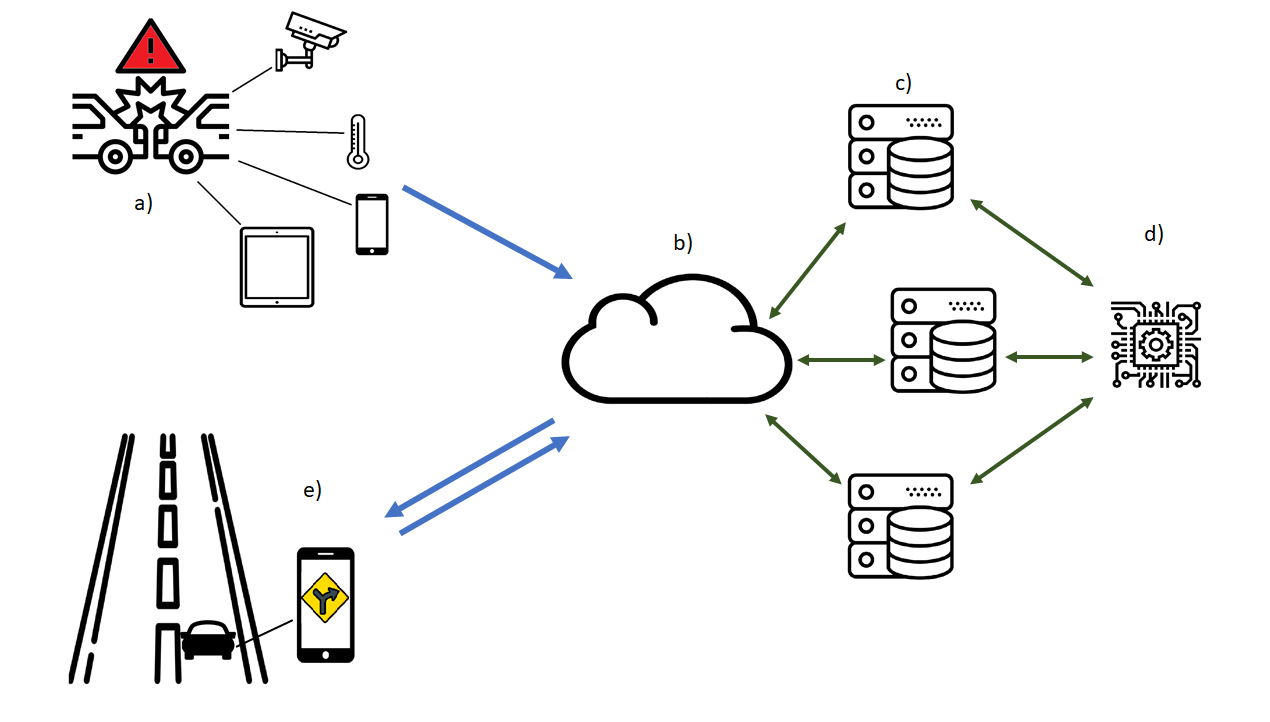
\includegraphics[width=0.8\columnwidth]{images/schema_fin}
	\end{center}
	\caption{Schema del prototipo. a) Raccolta dei dati attraverso un sistema eterogeneo di dispositivi. b) Condivisione dei dati in un Middleware IoT. c) Storing dei dati all'interno di Databases d) Analisi sui dati. d) Query Geo-Referenziata sulle condizioni di traffico. }
	\label{fig:application_schema}
\end{figure}

\section{La Raccolta dei Dati}
Il primo passo per l'implementazione di un sistema come quello proposto nella \autoref{sec:general_idea} è quello dello studio ed analisi dei dati necessari e la conseguente raccolta degli stessi. \\
Lo sviluppo delle tecnologie legate al mondo dell'IoT ha prodotto tutto un movimento tecnologico per la creazione di nuovi dispositivi e per il miglioramento di quelli esistenti. Questo ha consentito lo sviluppo di competenze tecnologiche nella realizzazione di unità di calcolo, circuiti integrati, sensori e strumenti di comunicazione sempre più avanzati ed economici. Questo movimento ha consentito inoltre di incrementare la diffusione di componenti elettroniche la cui potenza e costo li rendono disponibili all'utilizzo in qualsiasi applicazione. \\
In riferimento allo sviluppo di un sistema come quello ideato nella sezione \autoref{sec:general_idea}, si richiede che un numero molto elevato di sensori venga disposto sulla rete stradale in maniera capillare, così da poter avere dati affidabili ed in real-time sulla condizione del traffico in tutto il territorio. Alcuni di questi sensori sono già presenti ma sono in numero talmente basso che, con i dati da essi estratti, si potrebbero solamente ottenere informazioni parziali sul traffico su una porzione molto limitata del territorio.
\begin{figure}
	\begin{center}
		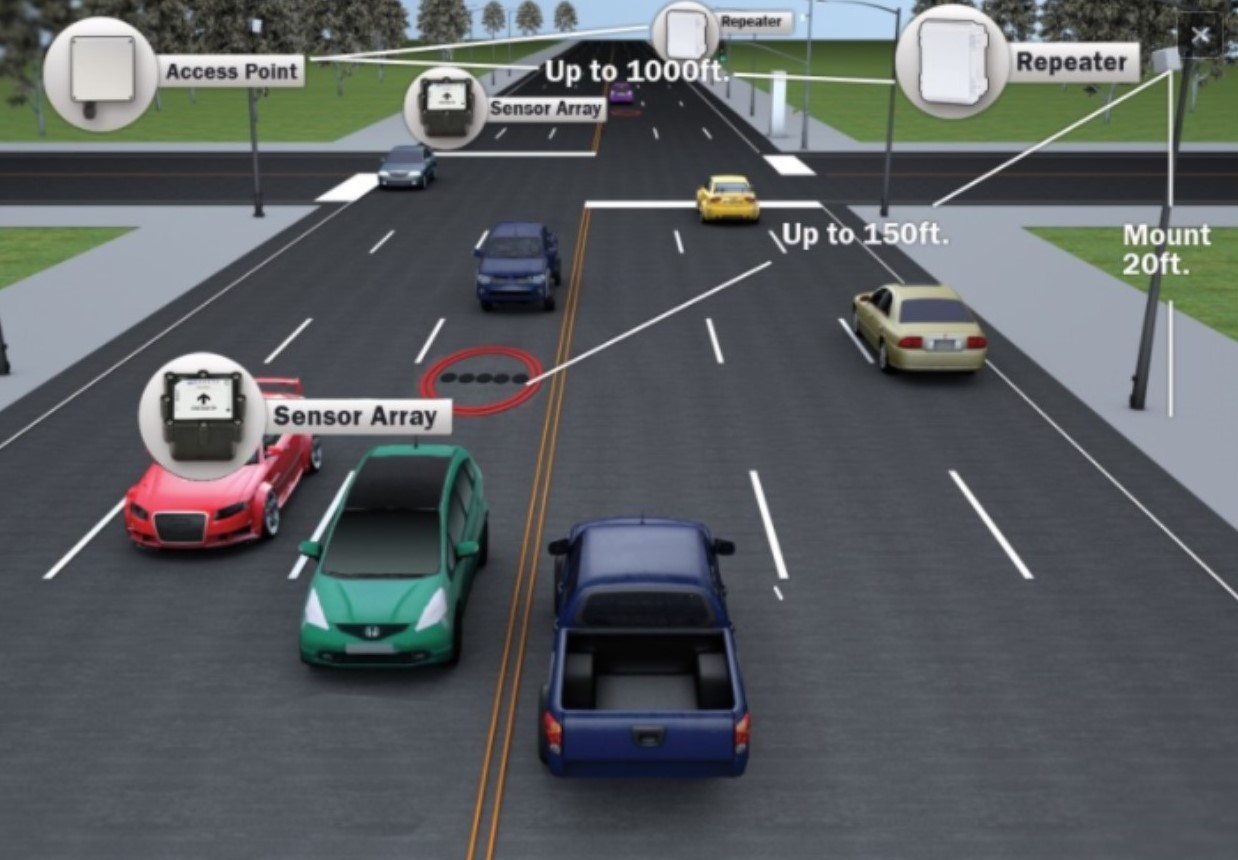
\includegraphics[width=0.7\columnwidth]{images/traffic_sensor}
	\end{center}
	\caption{Principio di funzionamento dei sensori attualmente in uso per la misura del livello di traffico}
	\label{fig:traffic_sensors}
\end{figure}
Le difficoltà principali nello sviluppo di una piattaforma per il controllo del traffico sono ovviamente quelle legate ai costi per la distribuzione di una rete di sensori che copra tutta la rete stradale.
Pertanto, è necessario trovare altre soluzioni che possano risultare più sostenibili ed anche scalabili.
Come evidenziato nel \autoref{chap:due}, uno dei principali vantaggi di una piattaforma di Crowdsourcing è proprio quello di garantire che, attraverso il contributo non organizzato dei singoli, si possa raggiungere un obiettivo comune riducendo di fatto i costi.\\
Attualmente, infatti, la rete stradale è già ampiamente invasa da un numero estremamente elevato di sensori i quali sono diffusi in maniera capillare e senza costi aggiuntivi: gli Smartphone (o Tablet). \\
Gli Smartphone sono il più evidente esempio della diffusione di componenti elettroniche  i quali, nelle loro evoluzioni hanno integrato al loro interno un numero sempre maggiore di sensori, diventando sempre più accurati e miniaturizzati.
\begin{figure}
	\begin{center}
		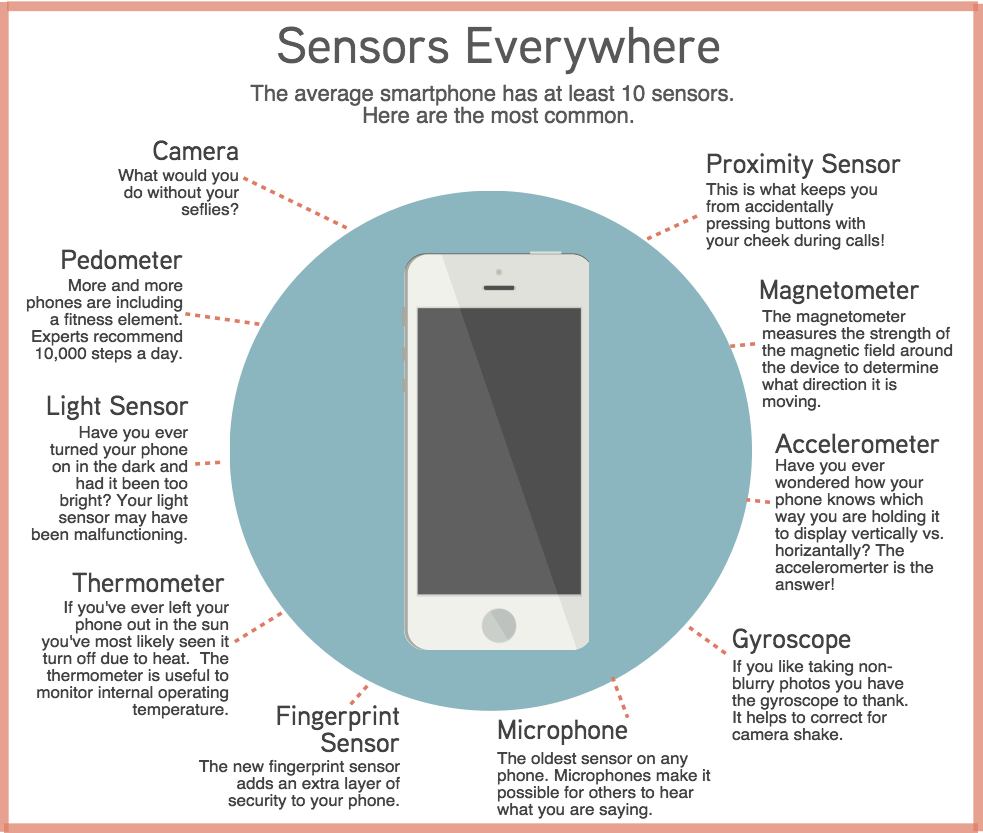
\includegraphics[width=0.8\columnwidth]{images/smartphone_sensors}
	\end{center}
	\caption{Crescita della disponibilità di sensori nell'equipaggiamento di uno smartphone fonte: CornerAlliance}
	\label{fig:smartphone_sensors}
\end{figure}
Sebbene il mercato degli smartphone sia molto eterogeneo dal punto di vista della dotazione hardware e del sistema operativo, generalmente si avranno sempre a disposizione alcune tipologie di sensori che possiamo classificare in funzione della grandezza fisica che essi misurano:
\begin{itemize}
	\item Termometro
	\item Accelerometro
	\item Giroscopio
	\item Microfono
	\item Camera
	\item GPS
\end{itemize}
Con l'aggiunta, in dispositivi più avanzati di:
\begin{itemize}
	\item[$\blacksquare$] Pedometro
	\item[$\blacksquare$] Prossimità
	\item[$\blacksquare$] Impronte Digitali
	\item[$\blacksquare$] Magnetometro
\end{itemize}
Effettivamente, la sensoristica di cui è dotato un singolo smartphone non sarebbe in nessun modo in grado di stimare autonomamente il livello del traffico o l'eventuale presenza di incidenti. Tuttavia, una piattaforma che raccolga i dati di un gran numero di dispositivi e che utilizzi degli algoritmi di analisi dei dati, sarebbe in grado di effettuare delle stime sul livello del traffico in un' area geografica. Questo è quello che viene proposto in \cite{famous:paper_smartphone_traffic_detection} dove viene analizzata una piattaforma per la raccolta dei dati relativi al traffico proveniente da un gran numero di smartphone e ne viene anche analizzato il rischio per la sicurezza di un utente che contribuisca ad una simile piattaforma dovendo condividere, tra gli altri, anche i dati relativi alla propria posizione.\\
Nel caso del prototipo ideato nella \autoref{sec:general_idea}, non si vuole soltanto realizzare una piattaforma che raccolga dati provenienti da smartphone, ma si vuole fare in modo che questa piattaforma sia adatta anche a raccogliere dati provenienti da infrastrutture stradali ed autostradali per il monitoraggio del traffico e per la comunicazione del livello di traffico. Si vuole cioè raccogliere in un'unica piattaforma i dati provenienti dai sensori stradali per il traffico come quello mostrato in \autoref{fig:traffic_sensors}, quelli provenienti da stazioni meteo, smartphone, tablet, computer di bordo di automobili, stazioni di monitoraggio del traffico e così via. Sebbene nella fase di prototipazione ci si focalizzerà principalmente sulla raccolta dati da smartphone e della conseguente trasmissione degli stessi secondo un predefinito formato, tutte le scelte progettuali sono pensate per essere compatibili anche per la raccolta dati dai diversi dispositivi precedentemente elencati.



\subsection{Accesso ai Sensori di uno Smartphone}
L'aumento del numero dei sensori, l'aumento della loro accuratezza ed affidabilità, ha portato alla nascita di servizi che utilizzassero tutte o alcune delle letture fornite dai sensori per offrire dei servizi all'utenza.\\
Alcuni di questi servizi consentono ad esempio di monitorare la qualità del proprio sonno, il numero di Kcal bruciate ogni giorno, regolare in modo automatico la luminosità e la gamma di colori del proprio schermo per salvaguardare gli occhi dell'utilizzatore ed una serie di altri infiniti servizi, tutti possibili sulla base dei dati provenienti da uno o più sensori.\\
\begin{figure}
	\begin{center}
		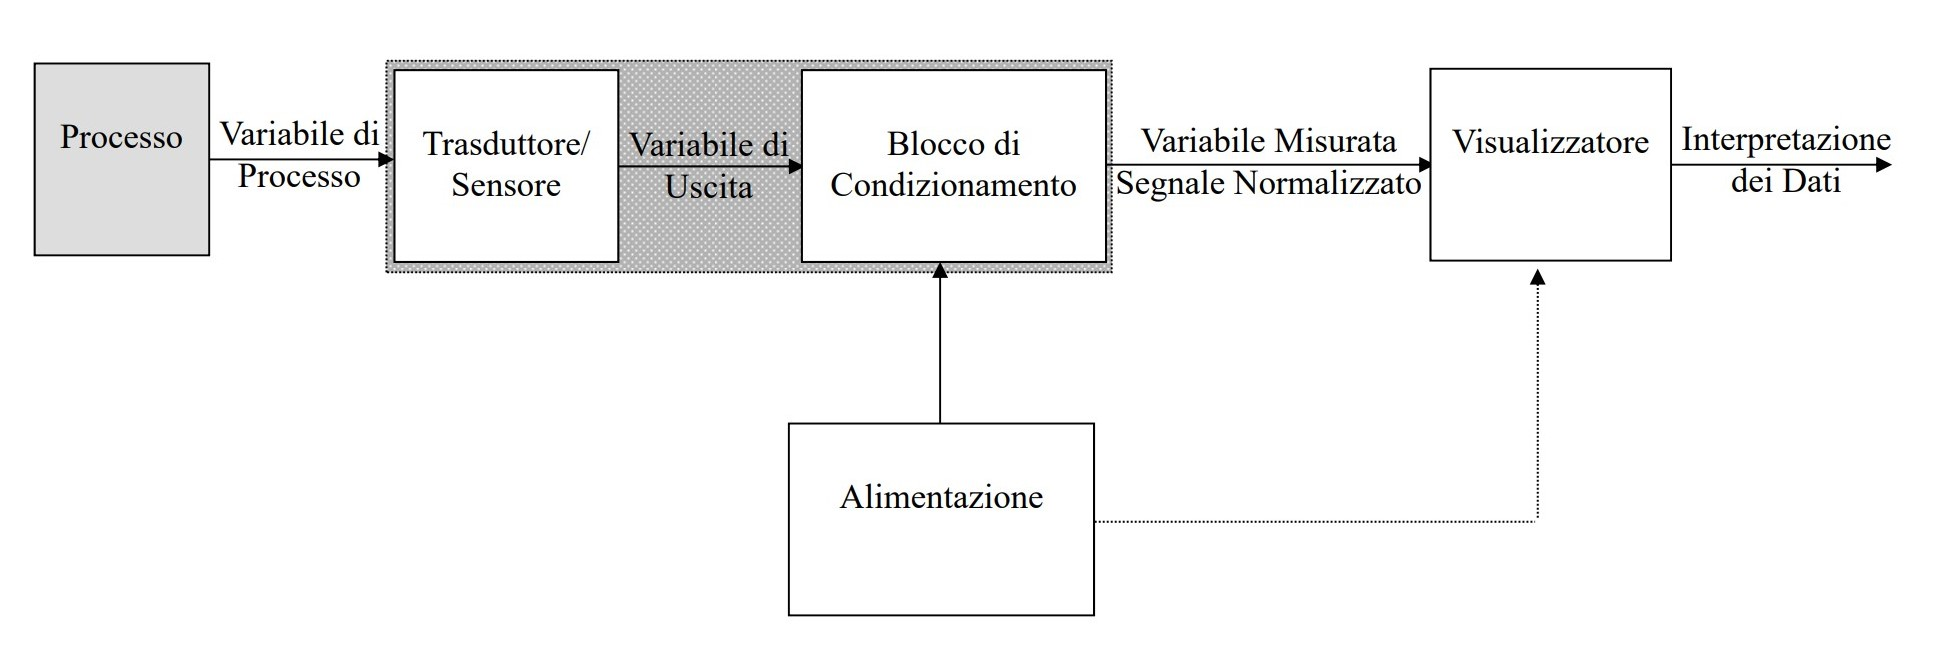
\includegraphics[width=0.9\columnwidth]{images/attivissimo}
	\end{center}
	\caption{Schema generale di un sistema di misura}
	\label{fig:attivissimo}
\end{figure}
\begin{figure}
	\begin{center}
		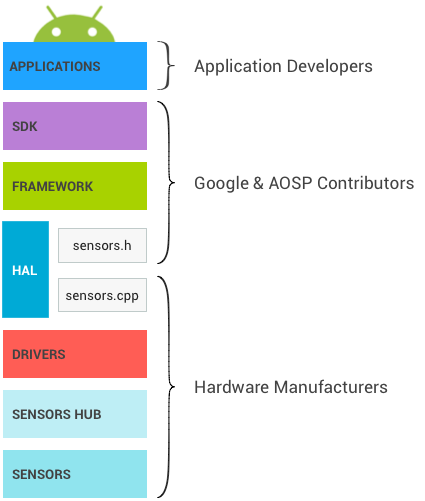
\includegraphics[width=0.55\columnwidth]{images/android_sensors}
	\end{center}
	\caption{Estratto dello stack utilizzato nel sistema operativo Android per rendere disponibili le letture dei sensori ad applicazioni e servizi}
	\label{fig:android_sensors}
\end{figure}
Questi servizi o applicazioni non sono altro che l'ultimo step di una struttura verticale nella quale, ai primi livelli si trovano effettivamente le componenti hardware del sensore che producono una uscita elettrica. Si rende necessario poi filtrare, amplificare e condizionare questo segnale elettrico al fine di renderlo comprensibile e trasmissibile come in \autoref{fig:attivissimo}. La variabile fisica o variabile di processo che si intende misurare viene quindi trasdotta o convertita in un'altra forma (generalmente elettrica) che è più semplice da trasmettere ed elaborare. Questa variabile di uscita prodotta dal blocco sensore e trasduttore non è tuttavia ancora adatta ad essere utilizzata. Questa subirà quindi un nuovo processo di condizionamento nel quale verrà filtrata, amplificata e linearizzata. Di qui il sistema operativo si occupa di interpretare ed eventualmente tradurre in un diverso formato le letture dei sensori in modo da renderle disponibili attraverso una interfaccia alle applicazioni e servizi dei livelli superiori che ne fanno richiesta. Tali applicazioni o service provider saranno quindi solo i consumatori finali di questi dati dai quali estrarranno le informazioni da mostrare all'utente finale che usufruisce del servizio.
Come evidente, nello stack utilizzato dal sistema operativo per smartphone Android \autoref{fig:android_sensors} viene offerto agli sviluppatori che realizzano servizi ed applicazioni una interfaccia diretta e standardizzata per l'utilizzo delle letture provenienti dai sensori. A prescindere dal sistema operativo utilizzato e dal tipo di sensori di cui è dotato lo smartphone, sarà offerto agli sviluppatori una interfaccia chiamata SDK ovvero Software Development Kit che indica un insieme di strumenti per lo sviluppo e la documentazione di software. In questo modo, coloro che si occupano di fornire servizi basati sulle letture di sensori, non dovranno preoccuparsi di elaborare, tradurre e condizionare l'uscita del sensore, ma solo di utilizzarla. \cite{developer:android} \cite{developer:apple}

\subsection{Parametri di Qualità dei Sensori}
\label{subsec:quality_param}
Ai sensori è generalmente richiesto di funzionare in ambienti ostili all'uomo e spesso ostili anche all'elettronica. Inoltre, un sensore sarà ritenuto tanto migliore quanto più esso riuscirà ad essere sensibile ad una sola grandezza ed insensibile a tutte le altre grandezze o rumore che possono disturbarne la misura. \cite{book:slide_Attivissimo} \cite{book:sensori_trasduttori} \\
Si può quindi sintetizzare che la \textbf{qualità di un sensore} sia determinata dalla sua sensibilità alla grandezza che si vuole misurare e dalla sua insensibilità a tutte le altre grandezze fisiche ambientali.
Essendo interessati alla valutazione delle prestazioni di un sensore in modo da poterne valutare la sua affidabilità e la qualità delle sue letture, va considerato che l'accurateza del dispositivo può variare con altre grandezze di influenza (temperatura, umidità, ecc.) e che spesso, si perviene alla misura di una grandezza fisica di interesse in maniera indiretta, introducendo così una propagazione del'errore.
\begin{figure}
	\begin{center}
		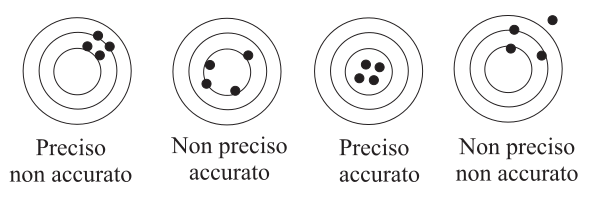
\includegraphics[width=0.9\columnwidth]{images/accuracy_precision}
	\end{center}
	\caption{Differenza tra la definizione di Precisione e quella di Accuratezza di una misura}
	\label{fig:accuracy_precision}
\end{figure}
Una prima valutazione sulla qualità di un sensore può essere effettuata attraverso due indici: \textbf{responsivity} e \textbf{detectivity}.\\
La \textbf{responsivity} o \textbf{sensitivity} rappresenta l'efficienza di trasduzione del sensore ed è normalmente espressa come il rapporto di due unità di misura, in genere differenti.
\begin{center}
	\begin{equation}
		r = \frac{\partial S\textsubscript{o}}{\partial S\textsubscript{i}} \quad \big[S\textsubscript{o} \textbackslash S\textsubscript{i}\big]
	\end{equation}
\end{center}
La \textbf{detectivity} rappresenta la capacità di un sensore di rendere disponibile un segnale dipendente dalla grandezza di ingresso e di tenerlo distinto dal rumore da esso stesso prodotto. Il suo valore dipende dal \textit{noise floor} ed è legato alla soglia o minimo segnale rilevabile. Si misura come il reciproco dell'unità di misura dell'ingresso.
\begin{center}
	\begin{equation}
	d = \frac{S\textsubscript{o}\textbackslash N\textsubscript{o}}{S\textsubscript{i}} = \frac{r}{N\textsubscript{o}} \quad \big[S\textsubscript{i} ^{-1}\big]
	\end{equation}
\end{center}
Queste informazioni, saranno utili al fine dello sviluppo del prototipo in quanto, dal momento che la piattaforma ideata nel \autoref{sec:general_idea} si occuperà di raccogliere i dati provenienti da un numero molto elevato di dispositivi eterogenei, questo significa anche che le letture dei sensori provenienti dai diversi sensori saranno qualitativamente eterogenee.\\
Pertanto, un primo requisito, sarà quello di valutare i parametri di qualità relativi alle letture dei sensori di ciascun dispositivo ed eseguire in questo modo un primo filtraggio dei dati in modo da escludere dall'analisi quelle letture affette da un grado di incertezza troppo elevato o non compatibile con l'analisi effettuata. Nel caso degli smartphone e tablet, queste informazioni sono messe a disposizione all'interno del SDK.

\subsection{Filtraggio delle Letture dei Sensori}
\label{subsec:filtering_sensor}
Nella \autoref{fig:attivissimo} è possibile notare come nel sistema di misura sia presente una componente che si occupi di filtrare, amplificare e linearizzare l'uscita fisica del sensore: il Blocco di Condizionamento. Questo blocco è generalmente di tipo software ed è realizzato ad-hoc per il particolare sensore e per il particolare utilizzo. Il suo scopo è quello di portare il segnale in uscita dal sensore in un formato compatibile con il dispositivo di elaborazione che lo segue riducendo al massimo gli effetti negativi di carico. \cite{book:slide_Attivissimo} Allo stesso modo, anche per quanto riguarda i sensori di cui sono dotati gli Smartphone, è necessario che le relative uscite vengano condizionate in maniera opportuna in funzione della particolare applicazione.\\
Prima però è necessario effettuare un approfondimento sui sensori che possono equipaggiare uno smartphone (e che sono necessari alla predizione delle condizioni stradali). All'interno degli smartphone, infatti, è possibile incontrare due diverse tipologie di sensori:
\begin{itemize}
	\item Sensori Hardware
	\item Sensori Software
\end{itemize}
Questa distinzione, sebbene non evidente all'utente finale, produrrà diverse tipologie di dati che dovranno quindi essere trattati diversamente.\\
I \textbf{Sensori Hardware} sono componenti fisiche che sono effettivamente montate all'interno di uno smartphone. Pertanto, le letture di questi sensori provengono dalla misura di una certa grandezza fisica attraverso un sistema di misura come quello mostrato in \autoref{fig:attivissimo}. Un esempio ne sono l'accelerometro, il magnetometro ed il sensore per l'intensità luminosa.\\
I \textbf{Sensori Software} non sono sensori fisici composti cioè da componenti elettroniche che trasducano una certa grandezza fisica. Questi sensori, emulano il comportamento di un sensore hardware ma le loro uscite sono spesso derivate da uno o più sensori hardware, opportunamente rielaborate via software. Un esempio ne sono sensore di orientamento, vettore di rotazione, pedometro.\\
Sebbene questa distinzione sia completamente invisibile a coloro che utilizzano questi dati e sia anche invisibile a coloro che sviluppano applicazioni e servizi sfruttando l' SDK messo a disposizione dal sistema operativo, è necessario tenerla a mente perchè i dati in uscita dalle diverse tipologie di sensori dovranno essere trattati diversamente. 
I dati in uscita dai sensori software sarnno infatti direttamente utilizzabili in quanto hanno già subito un processo di condizionamento proprio perchè, per definizione, sono derivati da altri sensori hardware.
Si rende invece necessario sviluppare un sistema di filtraggio ed eventualmente linearizzazione per le letture dei sensori hardware.\\
Il problema dei sensori hardware è che la frequenza con la quale le  uscite variano il loro valore è così elevata che, se mappassimo tutte queste piccole variazioni (Rumore), i valori oscillerebbero notevolmente. Più in generale, le letture provenienti dai sensori sono ricevute con una diversa frequenza ma, i picchi da essa raggiunti, sono troppo elevati.
\begin{figure}
	\begin{center}
		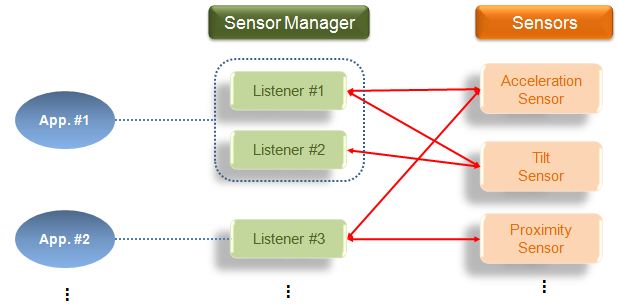
\includegraphics[width=0.9\columnwidth]{images/sensor_listener}
	\end{center}
	\caption{Principio con il quale nel sistema operativo Android è possibile recuperare le letture di un sensore ed utilizzarle in una applicazione. \cite{developer:android}}
	\label{fig:sensor_listener}
\end{figure}
Il processo che viene seguito nel sistema operativo Android per rendere disponibile la lettura di un sensore ad una applicazione o servizio che ne faccia richiesta è quello di instanziare un SensorListener il cui ruolo è appunto quello di restare in ascolto sull'uscita di un dato sensore e di notificare la applicazione nonappena venga rilevata una variazione del valore misurato dal sensore. La frequenza con la quale questo processo avviene dipende dalla velocità del sistema operativo e dalla capacità computazionale del dispositivo. Questo significa che dispositivi con una maggiore capacità di calcolo interrogheranno un numero maggiore di volte il sensore e riceveranno un numero maggiore di risposte affette, inevitabilmente, da rumore. Questo significa che è necessario utilizzare i soli valori necessari ed utili e filtrare il rumore.\\
La soluzione è l'applicazione di un filtro passa-basso sulle letture provenienti dai sensori in modo che esso consenta il passaggio alle sole basse frequenze del segnale e ne attenui il valore alle frequenze superiori a quella di taglio.\\
Si prenda ad esempio l'accelerometro di uno smartphone le cui letture indicano l'accelerazione del dispositivo rilevanta in un predefinito sistema di riferimento.
\begin{figure}
	\begin{center}
		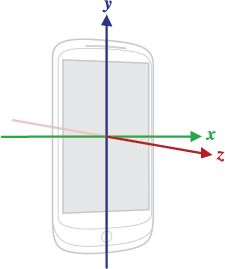
\includegraphics[width=0.3\columnwidth]{images/accelerometer}
	\end{center}
	\caption{Sensore di accelerazione a bordo di uno smartphone}
	\label{fig:accelerometer}
\end{figure}
A causa di un disturbo esterno come fattori ambientali o jerks o vibrazioni, viene aggiunto alla lettura del sensore una gran quantità di rumore. Queste componenti ad alta frequenza del segnale, provocano un'ampia oscillazione dei valori letti dal sensore. Questi disturbi, potrebbero essere tollerabili nella maggior parte delle applicazioni ma se si vogliono ottenere delle migliori letture è necessario progettare e sviluppare un filtro passa-basso che filtri a livello software le uscite di sensori hardware. In questo modo, è possibile filtrare le componenti di rumore ad alta frequenza utilizzando un opportuno valore di soglia.\\
\begin{lstlisting}[language=Java, label= code:low_pass_filter, caption=Pseudo-codice relativo all'implementazione di un filtro passa-basso]
for i from 1 to n
	y[i] :=y [i-1] + a*(x[i] - y[i-1])
end
\end{lstlisting}
Il \autoref{code:low_pass_filter} corrisponde ad una implementazione di un filtro passa-basso che prenda l'uscita \textit{y} di un sensore e la filtri con un filtro passa-basso avente \textit{a} come coefficiente di soglia.
La scelta del parametro \textit{a} dipende da quanto si intende dimensionare la frequenza di taglio del filtro. Quanto più essa sarà alta, tanto più rumore entrerà nel filtro viceversa, quanto più sarà bassa tanto più lento sarà il segnale. In \cite{developer:android} viene proposta una soluzione intermedia con la scelta del parametro \textit{a = 0.25}.

\section{Il Protocollo DATEX}
La raccolta dei dati è solo una piccola porzione del problema. Per ottenere il massimo da questi dati è necessario condividerli in modo da sfruttare le potenzialità delle piattaforme di Crowdsourcing nelle quali, le analisi effettuate su un gran numero di dati potrebbero fornire delle deduzioni e previsioni molto più accurate e significative.
Si rende quindi necessaria una comunicazione tra i dispositivi che si occupano della raccolta dati.\\
Diventa quindi necessario abilitare la comunicazione tra tutti i diversi dispositivi che si occupano della raccolta dati considerando la loro eterogeneità in termini di:
\begin{itemize}
	\item Capacità computazionale
	\item Sensoristica a disposizione
	\item Grandezze fisiche misurate
	\item Qualità delle letture dei sensori
	\item Costruttore del dispositivo
\end{itemize}
DATEX (da Data Exchange) è il protocollo che abilita la comunicazione tra dispositivi eterogenei per la condivisione di dati legati al traffico stradale ed autostradale. Questo protocollo fa in modo che differenti dispositivi possano comunicare tra loro e con un Middleware, definendo cioè uno Standard per la comunicazione condiviso tra tutti i partecipanti alla comunicazione.\\
Nella fattispecie, DATEX è il linguaggio utilizzato nella Comunità Europea per lo scambio di informazioni legate al traffico in modo da consegnare informazioni comprensibili all'utenza finale. DATEX è infatti stato progettato e sviluppato come un sistema per lo scambio di dati dalla Comunità Europea per la standardizzazione dell'interfaccia di comunicazione tra i gestori di strade ed autostrade, i produttori dei dati in strade ed autostrade e gli utilizzatori dei servizi sul traffico. \cite{famous:paper_datexii}\\
Una prima versione del Protocollo DATEX I è stata iniziata già nel 1990 mossa dalla necessità di un meccanismo per lo scambio di dati tra centri per il monitoraggio del traffico e gli operatori stradali. Ben presto, tuttavia, dato lo sviluppo tecnologico del XXI secolo, è sorta la necessità di integrare in questo standard anche i fornitori di servizi. Per questo motivo, viene sviluppato lo standard DATEX II con lo scopo di distribuire le informazioni sul traffico indipendentemente dalla lingua e dall'aspetto. In questo modo, viene eliminata la probabilità che nascano delle incomprensioni o errori di traduzione.\\
\begin{figure}
	\begin{center}
		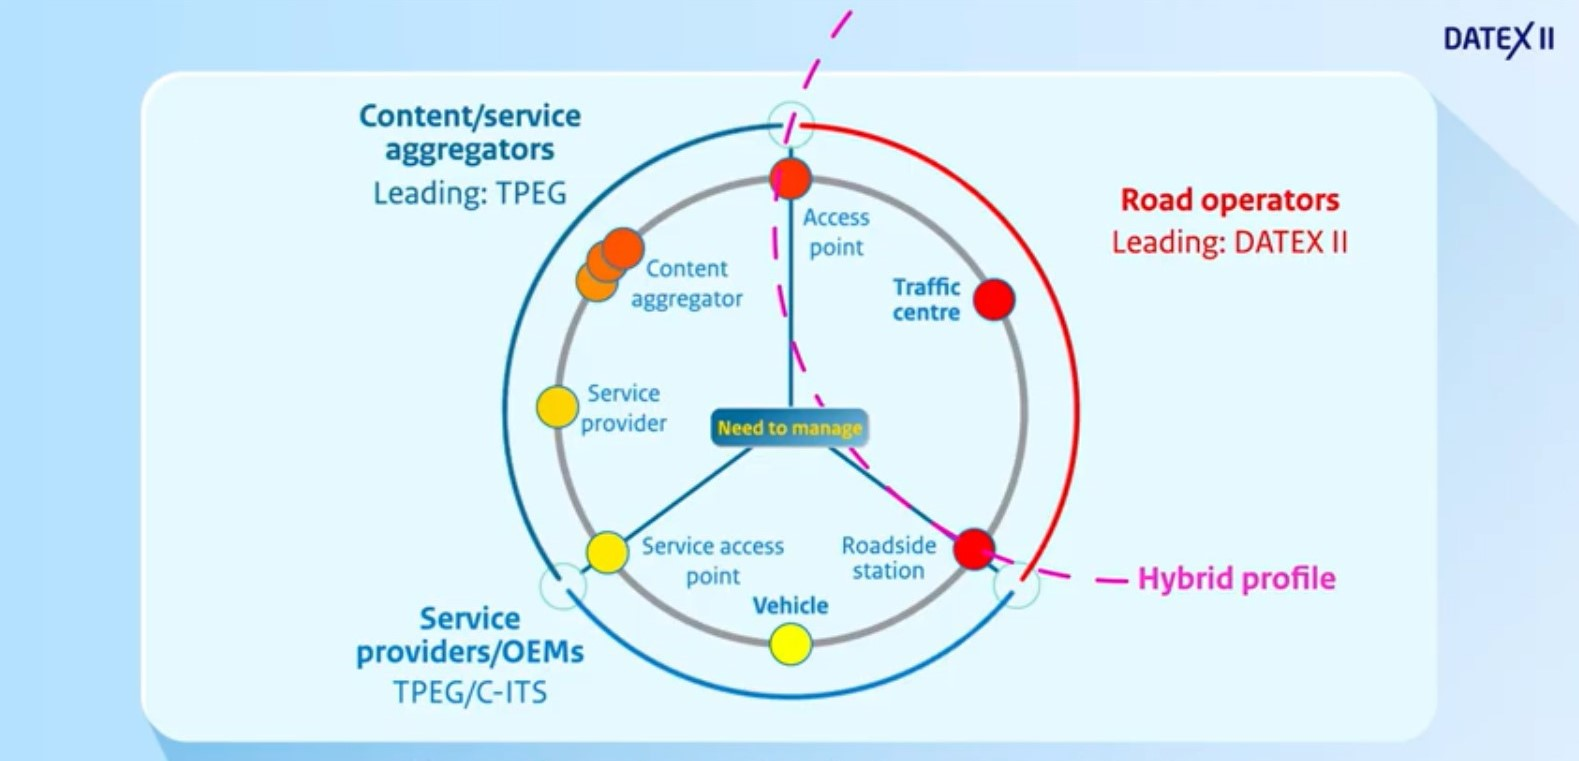
\includegraphics[width=0.8\columnwidth]{images/datexii}
	\end{center}
	\caption{Panoramica del Mondo ITS e le relative sfide tecnologiche}
	\label{fig:datexii}
\end{figure}
\begin{table}
	\begin{center}
		\begin{tabular}{|l|l|}
			\hline
			\textbf{Type} & \textbf{Remarks} \\
			\hline
			\pbox{20cm}{Accidents \\ Obstruction \\ Activities \\} & public events, police operations etc.  \\
			\hline
			\pbox{20cm}{Abnormal Traffic \\ Driving conditions \\ Poor road infrastructure \\ Network Management \\ Sign information \\ Roadside Assistance \\ Car parking information \\ Transit information \\ Service disruption \\} & \pbox{20cm}{Queues \\ Weather, Road surface \\ Closures, Restrictions \\ VMS settings \\ Number of vacant spaces \\ Rail and Ferry connections \\ Motorway service area} \\
			\hline
			\pbox{20cm}{Measured Traffic Data \\ Measured weather/pollution  \\} & \pbox{20cm}{Travel times, Flow data \\ Wind, precipitation, visibility, air quality} \\
			\hline
			\pbox{20cm}{Traffic View  \\} & \pbox{20cm}{Combination of event informations and URLs for CCTV cameras} \\
			\hline
		\end{tabular}
		\caption{Le metodologie di comunicazione \cite{famous:paper_datexii_research}}
		\label{tabel:datexii_data}
	\end{center}
\end{table}
Lo Standard DATEX II non è stato pensato per fornire delle rigide specifiche di comunicazione ma piuttosto come un Protocollo che ammettesse una certa libertà di scelta e che fosse in grado di evolversi per consentire, in futuro, lo scambio di informazioni aggiuntive.\\
Il dominio di dati che possono essere scambiati attraverso DATEX II riguarda tutti i dati relativi al trffico ed alle informazioni sul viaggio per strade urbane ed inter-urbane. Spaziando tra eventi legati al trffico come incidenti e lavori stradali ad eventi legati al flusso di traffico come permanenza sulle strade e durata del viaggio. \\
Risultano quindi evidenti le motivazioni che hanno portato alla scelta dello standard DATEX II nella progettazione del prototipo ideato in \autoref{sec:general_idea}. Rispetto ad altri protocolli di comunicazione, infatti, DATEX II presenta delle caratteristiche che ben si adattano allo scopo:
\begin{enumerate}
	\item Sviluppato, Supportato ed Utilizzato dalla Comunità Europea
	\item Progettato per lo scambio di dati relativi al traffico
	\item Supporta lo scambio dati tra dispositivi eterogenei
	\item Indipendente dalla tecnologia utilizzata per lo scambio dati
	\item Flessibile per adattarsi a nuove necessità e dati da scambiare
	\item Geo-Referenzia i dati scambiati tra i vari dispositivi
	\item Documentazione completa per gli sviluppatori che vogliano integrare il protocollo nelle loro applicazioni
	\item Documentazione completa per gli sviluppatori che vogliano ampliare il protocollo in funzione di nuove necessità
\end{enumerate}
Progettando quindi il sistema della \autoref{sec:general_idea} in modo che supporti il protocollo DATEX II, si fa in modo che il sistema possa essere aperto a ricevere non solo i dati provenienti da altri smartphone o tablet sui quali è installato lo stesso sistema, ma anche da Centri per il controllo del traffico, infrastrutture stradali e centri di informazione su tutta la rete stradale Europea, avendo così a disposizione un più ampio data-source sulla base del quale effettuare previsioni, analisi ed inviare comunicazioni agli utenti.

\subsection{DATEX II Data Model}
\label{sec:datexii_data_model}
Il principale vantaggio del Protocollo DATEX II è la sua flessibilità che lo rende a prova di futuro. Questa caratteristica viene fornita allo standard da un ricco ed ampiamente sviluppato modello dei dati in formato UML (Unified Modeling Language). Questo consente allo Standard DATEX II di avere un modello dei dati che sia indipendente dalle sue implementazioni e che quindi possa essere mappato diversamente in diverse implementazioni.
Attualmente, questo modello dei dati è mappato in informazioni codificate attraverso XML (eXtensible Markup Language) con la creazione di un XML schema. XML e XML schema sono tra i sistemi per la definizione dei modelli di dati più ampiamente utilizzati. Questa scelta garantisce che l'interfaccia DATEX II sia facilmente integrabile in quante più implementazioni ed applicazioni possibili.\\
In più, DATEX II implementa un alto livello di flessibilità attraverso una opzione di estensibilità del modello dei dati. Questo consente ad utenti singoli di scambiare dati attraverso il modello dei dati DATEX II, ma che sia stato adattato alle loro particolari necessità e preferenze, rimanendo comunque conforme allo standard DATEX II. Questo viene reso possibile offrendo agli utenti la possibilità di ampliare il modello dei dati di DATEX II, seguendo una definita procedura, in modo che si mantenga l'interoperabilità con altri dipositivi e centri di controllo per il traffico che utilizzino una qualsiasi altra implementazione conforme a DATEX II. \cite{famous:paper_datexii_research}\\
Lo sviluppo do DATEX II si è focalizzato sulla creazione di un documento di riferimento nel quale viene posta particolare enfasi alla distinzione tra Data (contenuto) e Meccanismo di Scambio. La descrizione tecnica fornisce una chiara distinzione tra Platform Independent Modelling (PIM) e Platform Specific Modelling (PSM). PIM si riferisce al dominio dei dati scambiati relativi al traffico mentre PSM si riferisce alle specifiche informazioni scambiate ed alla tecnologia di comunicazione utilizzata.
Questa separazione tra i due domini produce una migliore comprensione dello standard rendendolo più facile da applicare.

\subsubsection{Level A - Data Model}
DATEX II viene sviluppato a valle di un periodo di studio ed osservazione sul tipo e numero di dati che sono scambiati dai dispositivi IoT nella Comunità Europea. Risultato di questa osservazione è il modello dei dati in formato UML di DATEX II anche noto con il termine "Level A Data Model". Sebbene ampiamente completo e documentato, potrebbero ancora esserci delle situazioni nelle quali l'interfaccia dati richiesta da un particolare utente possa non essere presente nel Data Dictionary di DATEX II in quanto, ad esempio, sono dati riferiti ad un contesto nazionale o locale.\\
In questo caso, questi utenti sono in  grado di fornire una estensione al modello che includa i concetti mancanti, nota anche come "Level B Extension Model". Agli utenti viene quindi data la possibilità di aggiungere una limitata estensione al diagramma UML, seguendo predefinite istruzioni. Queste estensioni (Level B) devono comunque mantenere l'interoperabilità con lo standard DATEX II in modo che altri dispositivi che siano compatibili con DATEX II (ad esempio con il Level A), possano ancora mantenere una interoperabilità e che cioè siano in grado di processare i dati (o Publications) provenienti da un dispositivo che implementi un modello dei dati personalizzato (ad esempio di Level B), senza essere ovviamente in grado di processare i dati aggiunti dal particolare client.\\
Soltanto altri client specializzati, che cioè implementano tutto il modello dei dati modificato (di Level B) saranno in grado di processare tutto il contenuto, comprese le estensioni.\\
Lo scopo principale per cui il Level B è progettato riguarda i soli casi in cui uno specifico utente implementi ed utilizzi il modello dei dati di Level A per la maggior parte delle comunicazioni ma che, in alcuni casi, non sia sufficiente a soddisfare le proprie necessità e risulta necessario ampliarlo.\\
Questo tuttavia non comprende il caso nel quale si vogliano definire dei concetti che siano completamente nuovi o completamente fuori dallo scope del Level A. In questo caso, gli utenti che dovessero incorrere in tali necessità hanno ancora la possibilità di ampliare il modello dei dati nel diagramma UML così da avere ancora un certo livello di interoperabilità. Questi modelli così modificati sono chiamati "Level C Extensions". Le implementazioni che forniscano dei dati (o Publications) di Level C non sono generalmente in grado di essere interoparabili con le implementazioni di Level A o Level B.
.
\subsubsection{Level B - Extension Mechanism}
Sebbene il Level A sia già abbastanza ricco ed il suo modello dei dati abbastanza completo, non è escluso che nel tempo possano sorgere delle nuove necessità o applicazioni che vogliano aggiungere nuovi concetti ed attributi al modello esistente. Al fine di rendere il Protocollo DATEX II adatto a sopravvivere alle innvovazioni nel tempo, è stato progettato un meccanismo formale attraverso il quale il modello dei dati di Level A puù essere esteso. E' necessario che queste nuove applicazioni che estendono il Level A, chiamate Level B, mantengano una compatibilità con il DATEX II nella sua versione base (Level A). Questo consente alle nuove implementazioni dello standard che arricchiscano il Level A con l'aggiunta di nuovi concetti o attributi di restare comunque compatibili con lo standard nella sua versione base e quindi di interpretare correttamente le publications.
Fornitori o Client che volessero utilizzare completamente le informazioni definite in queste estensioni al Level A devono invece implementare il modello dei dati definito nell'estensione stessa Level B e non il solo modello base Level A.\\
Presso \url{www.datex2.eu} è disponinbile un processo di registrazione di nuove estensioni di tipo B allo standard DATEX II. Qualora queste estensioni dovessero raggiungere ampio consenso, saranno integrate direttamente nella versione base dello standard.

\subsubsection{Level C - Extensions}
Dopo aver analizzato le possibilità offerte dalle versioni A e B dello standard DATEX II e dalla loro intercompatibilità, alcuni utenti potrebbero ancora ritenere necessario un ampliamento ancora più profondo dello standard con l'aggiunta di nuove ddefinizione e di nuovi scope. Queste modifiche potrebbero anche rivelarsi troppo distanti dal modello dei dati di Level A e quindi non implementabili con una sola estensione del Level A in Level B. Per questo motivo, viene anche sviluppato il concetto di Level C le cui implementazioni sono considerate non conformi allo standard e quindi non interoperabili con i Level A, B. Nonostante questa incompatibilità, le implementazionid i Level C devono quantomeno utilizzare le regole di modelling e protocolli di scambio dati che siano comuni a DATEX II.
Questo potrebbe consentire in futuro uno scambio di idee e portare alla creazione di un modello dei dati unificato.

\subsubsection{Data Dictionary}
Lo standard DATEX fornisce le definizioni di quelli che sono i concetti e gli attributi utilizzati nel modello dei dati in modo da aiutare gli sviluppatori nell'utilizzo ed implementazione dello Standard. Queste definizioni sono raccolte in un diagramma UML per gli addetti ai lavori ed in un file Excel che documenti tutte le definizioni in una forma più comprensibile. In questo modo, è possibile istantaneamente valutare se lo standard comprenda già tutti gli attributi necessari alla particolare istanza o se sia necessario aggiungerne di nuovi.

\subsection{XML Schema}
Il formato XML sta vedendo una notevola crescita del suo utilizzo per lo scambio di informazioni. Una componente fondamentale di questo approccio sono gli XML Schemas. Basandosi su un modello dei dati e su un dizionario dei dati, gli XML Schemas sono progettati per adattarsi ad una particolare area applicativa. Questi schemi sono degli strumenti per capire il contenuto dei dati che sono scambiati.\\
Il modello UML viene inizialmente esportato in un file XMI ed in seguito, attraverso un tool di conversione, viene trasformato in un XML Schemas.
Questi XML Schemas sono utilizzati per lo sviluppo sofwtare. XMI (XML Metadata Interchange) è invece uno standard OMG per lo scambio di metadati in formato XML. L'uso più comune che se ne fa di XMI è proprio quello di interscambio di modelli UML.
\begin{figure}
	\begin{center}
		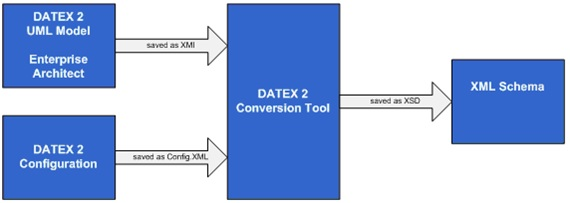
\includegraphics[width=0.8\columnwidth]{images/datexii_xml}
	\end{center}
	\caption{Workflow di un processo di conversione automatico}
	\label{fig:datexii_xml}
\end{figure}

\subsection{Exchange Mechanisms}
Ci si focalizza ora su quali metodologie sono supportate dal protocollo DATEX II per lo scambio dei dati tra i diversi dispositivi che partecipano alla piattaforma. \\
DATEX II offre metodologie di push e pull per lo scambio di informazioni. \\
La modalità \textbf{push} consente al fornitore di inviare le informazioni al client. Questa operazione può essere effettuata periodicamente ad intervalli di tempo regolari oppure all'occorrenza quando il fornitore dovesse ritenerlo opportuno.\\
La modalità \textbf{pull} consente al client di richiedere dati ad un fornitore.\\
Una descrizione di alto livello di come avvenga la comunicazione tra fornitore e consumatore dei dati, senza considerare i dettagli tecnici, può essere sintetizzata in tre operazioni principali:
\begin{enumerate}
	\item \textbf{Publisher Push on Occurrence: } La comunicazione e l'invio dei dati viene cominciata dal publisher ogni volta che i dati cambiano
	\item \textbf{Publisher Push Periodic: } La comunicazione e l'invio dei dati viene cominciata dal publisher ad intervalli di tempo regolari
	\item \textbf{Client Pull: } La comunicazione viene cominciata dal Client che si aspetta l'invio dei dati richiesti come risposta dal Publisher
\end{enumerate}
Le metodologie di comunicazione viste finora possono essere sia online che offline. Nel Platform Specific Modelling (PSM), la sezione relativa allo scambio dei dati è stata progettata per essere indipendente dal contenuto che viene scambiato, ovvero dal payload. In questo modo, le informazioni relative allo scambio dei dati possono essere studiate indipendentemente dal modello dei dati in formato UML di DATEX II, garantendo così la separazione dei due campi.\\
Questa separazione logica ed implementativa, non solo rende più facile la comprensione e l'applicazione del protocollo stesso, ma rende anche possibile riutilizzare una delle due sezioni qualora l'altra dovesse cambiare ed evolversi nel tempo per adattarsi a nuove necessità. Ad esempio, potrà variare nel tempo il modello dei dati dello standard DATEX II perchè potrebbero essere proposte delle nuove estensioni dello standard, tuttavia, non è necessario che vari anche il meccanismo di scambio dati in quanto indipendente dal payload.

\subsection{Exchanged Data}
Prima di analizzare nel dettaglio come sia fatto il diagramma UML relativo allo Standard DATEX II ed implementarlo nel sistema che prototiperà lidea della \autoref{sec:general_idea}, si analizzino più nel dettaglio i dati relativi al traffico che sono supportati dallo standard.\\
Questi dati che vengono scambiati, sono composti da elementi base che sono disponibili all'interno di una pubblicazione o alternativamente potremmo dire che tra i dispositivi viene scambiata una publication composta da elementi o attributi base.

\subsubsection{Elementi Base}
Una Publication in DATEX II è composta da elementi base che possiamo raggruppare in macro-categorie: 
\begin{enumerate}
	\item Eventi relativi a condizioni stradali e traffico ("Traffic Elements")
	\item Azioni dell'Operatore
	\item Incidenti
	\item Dati misurati o elaborati (tempo di viaggio, velocità del traffico stimata, intensità del traffico stimata, rilevazioni metereologiche, ...)
	\item Messaggi mostrati sui Variable Message Signs (VMS)
	\item Informazioni di Servizio (assenza di corsie di emergenza, ritardi su treni, ...)
\end{enumerate}
In più, sono anche presenti elementi come: Zone di Posteggio, Posizioni dei pannelli VMS e Posizioni dei siti di misura. 
Queste infromazioni, sebbene non siano dei dati elementari, sono comunque necessarie al Client al fine di comprendere ed utilizzare correttamente le informazioni degli elementi base.

\subsubsection{Eventi relativi a condizioni stradali e traffico}
Questi eventi riguardano tutti situazioni che non sono inizializzate da un operatore del traffico ma che lo obbligano ad intraprendere una decisione su come affrontare l'evento. Possono essere classificati in:
\begin{itemize}
	\item Traffico Anormale (lunghe code, rallentamenti)
	\item Incidenti
	\item Attività (eventi pubblici, disturbi al normale funzionamento)
	\item Condizioni Stradali. Possono essere o meno legate a condizion atmosferiche o all'ambiente
	\item Ostruzioni
	\begin{itemize}
		\item presenza di animali
		\item presenza di veicoli in panne
		\item ostruzioni dovute dall'ambiente (alberi)
		\item ostruzioni dovute a infrastrutture (caduta di cavi)
		\item ostruzioni dovute a persone
	\end{itemize}
	\item Incidenti ad infrastrutture o sistemi stradali (VMS guasti)
\end{itemize}

\subsubsection{Azioni dell'Operatore}
Riguardano eventi che sono inizializzati da un operatore del traffico e possono essere classificati in:
\begin{itemize}
	\item Manutenzione (chiusura di strade, traffico alternato)
	\item Lavori stradali (limiti temporanei, deviazioni)
	\item Assistenza a bordo strada
\end{itemize}

\subsubsection{Incidenti}
Questa sezione contiene in particolar modo gli eventi relativi alla disponibilità di corsie, rallentamenti ed eventuali deviazioni.

\subsubsection{Dati Misurati o Elaborati}
Questo set di dati può essere derivato da input diretti di stazioni per il traffico o strumentazione di uno specifico sito di misura, i quali dati possono essere ricevuti periodicamente o possono essere inviati in funzione delle condizioni di traffico in una specifica località.
\begin{itemize}
	\item Valori di Traffico misurati
	\begin{itemize}
		\item flusso
		\item velocità
		\item progresso
		\item concentrazione dei veicoli in coda		
	\end{itemize}
	\item Stato del traffico
	\begin{itemize}
		\item flusso libero, intenso, congestionato, sconosciuto
	\end{itemize}
	\item Tempo di viaggio
	\begin{itemize}
		\item tempo stimato
		\item tempo di viaggio nominale atteso
	\end{itemize}
	\item Condizioni Atmosferiche
	\begin{itemize}
		\item precipitazioni, vento, temperatura, inquinamento, condizioni del manto stradale e visibilità.
		\item previsioni metereologiche
	\end{itemize}
\end{itemize}

\subsubsection{Messaggi mostrati sui VMS}
Questo set di dati include diversi messaggi che possono essere mostrati sui differenti VMS (Variable Message Signs) in funzione della tecnologia che utilizzano, immagini e testo. Possono anche includere informazioni sulla posizione dei dispositivi VMS e sul loro status.

\subsubsection{Informazioni di Servizio}
Riguardano informazioni su un servizio che potrebbe influenzare il comportamento dei guidatori e quindi le caratteristiche del traffico.
\begin{itemize}
	\item  Informazioni sul Transito dei veicoli
	\begin{itemize}
		\item informazioni circa altri mezzi di trasporto (treni, tram, voli)
	\end{itemize}
	\item Indisponibilità di servizi (aree di sosta chiuse, aree di rifornimento chiuse)
	\item Indisponibilità di servizi stradali (chiamate di emergenza fuori uso)
\end{itemize}

\subsection{Publication di Elementi Base}
\label{sec:publication_base_element}
Gli elementi base mostrati in precedenza, possono essere scambiati individualmente tra dispositivi che implementano lo standard DATEX II o possono anche essere scambiati in gruppi di elementi. Questi scambi di gruppi di elementi base prendono il nome di Publication e, in funzione dei dati trasmessi, possono esserci cinque tipi fondamentali di Publication:
\begin{enumerate}
	\item \textbf{Situation Publication: } Usata per Elementi legati al traffico, azioni dell'operatore, incidenti o informazioni di servizio
	\item \textbf{Elaborated Data Publication: } Usata per lo stato del traffico, per i tempi di viaggio e per valori misurati di traffico e condizioni atmosferiche
	\item \textbf{Measured Data Publication: } Usata per Misure del traffico e rilevamenti atmosferici, stato del traffico e tempo di viaggio
	\item \textbf{Parking Publication: } Usata per le informazioni su parcheggi ed aree di sosta
	\item \textbf{VMS Publication: } Usata per i messaggi da mostrare sui VMS e sulle informazioni relative agli VMS.
\end{enumerate}

\subsection{Utilizzo del DATEX II Data Model}
Nelle sezioni precedenti, servendosi della documentazione ufficiale messa a disposizione dallo Standard DATEX (\url{https://datex2.eu/}), si sono evidenziati i vantaggi nell'adozione del protocollo ed anche le sue peculiarità implementative. Data la flessibilità offerta dal protocollo, risulta necessaria ora una fase di analisi su quelle che siano le caratteristiche del protocollo che è necessario implementare all'interno del sistema. Già da una prima analisi sull'idea del prototipo da realizzare, risulta subito evidente che sia superfluo implementare il protocollo DATEX II nella sua interezza in quanto, non tutte le sue componenti saranno necessarie al sistema. \\
Il punto di partenza di questa analisi è quello di adottare il Processo Unificato (UP) con il quale produrre la documentazione necessaria allo sviluppo del software relativo al sistema che si vuole implementare definito nella \autoref{sec:general_idea}. A tal proposito, è bene introdurre brevemente il Processo Unificato ed in generale gli strumenti messi a disposizione dall'Ingegneria del Software che saranno utilizzati nei capitoli seguenti.

\subsubsection{Il Processo Unificato}
Il Processo Unificato (UP) è uno dei modelli messi a disposizione dall'Ingegneria del Software che fornisce una sequenza di fasi da seguire per la progettazione e realizzazione di Software dalle grandi dimensioni. Il Processo Unificato e gli altri modelli per lo sviluppo di Software definiscono la lista di operazioni da seguire al fine di ottenere un prodotto software composto dal suo eseguibile, più la documentazione ad esso associato. Risulta infatti necessario, per software dalle grosse dimensioni, documentare ogni singola fase dello sviluppo, comprese quelle di progettazione.\\
Nello sviluppo di questo particolare sistema, la scelta è ricaduta sul Processo Unificato in quanto questo modello sia particolarmente flessibile ed adatto alla modellazione visuale attraverso l'Unified Modelling Language (UML) che è la stessa tipologia di modellazione utilizzata dallo standard DATEX II. In questo modo, sarà più semplice integrare il Software che si intende sviluppare in questo lavoro di tesi con il Protocollo DATEX II.\\
Il Processo Unificato si compone di diverse fasi, nelle quali ci si focalizza su vari aspetti del processo software e tra le quali fasi si può ciclicamente iterare per implementare nuove funzionalità del Software:\\
\begin{enumerate}
	\item \textbf{Ideazione: } Fornisce una visione approsimativa del progetto. Stime sul progetto di carattere economico e relative alle tempistiche.
	\item \textbf{Elaborazione: } Viene raffinata la visione del progetto, vengono identificati la maggior parte dei requisiti e sono realizzate delle stime più realistiche del progetto.
	\item \textbf{Costruzione: } Fase di implementazione iterativa degli elementi rimanenti e preparazione al rilascio.
	\item \textbf{Transizione: } Beta test e Rilascio agli utenti.
\end{enumerate}
\begin{figure}
	\begin{center}
		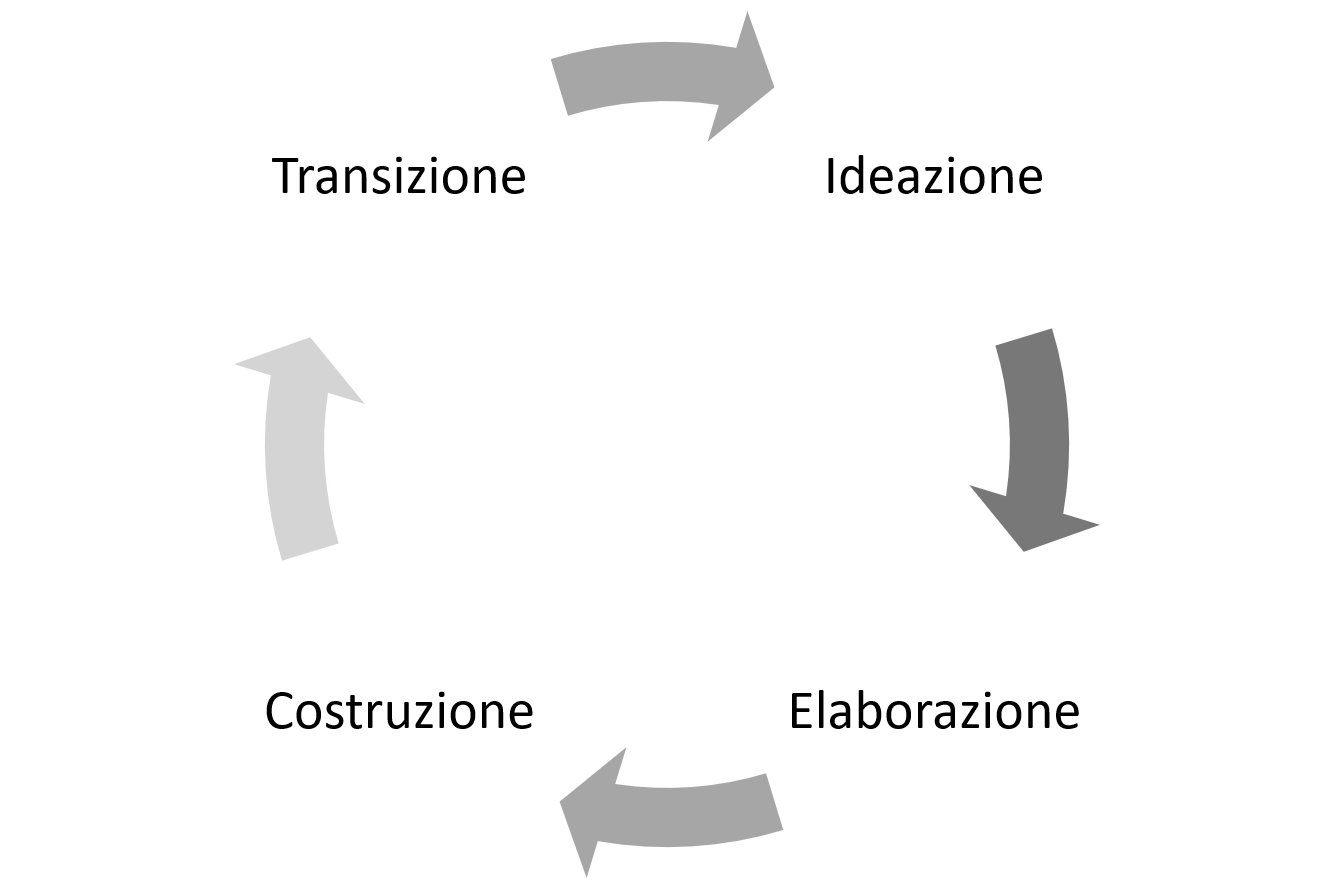
\includegraphics[width=0.5\columnwidth]{images/up}
	\end{center}
	\caption{Fasi del Processo Unificato}
	\label{fig:up}
\end{figure}
Nella fattispecie, si produrrà in questo lavoro di tesi una parte della documentazione prevista dal Processo Unificato per la realizzazione del Software che prototiperà l'idea descritta nella \autoref{sec:general_idea} che sarà di supporto alla progettazione e sviluppo del Software ed alla sua comprensione ed il suo adammento a nuove applicazioni. \cite{book:slide_Nocera}, \cite{book:software_engineering}

\subsubsection{Requisiti Funzionali}
Uno dei documenti che è necessario produrre se si vuole intraprende l'utilizzo del Processo Unificato è l'Analisi dei Requisiti Funzionali. I Requisiti di un Software possono infatti essere suddivisi in:
\begin{itemize}
	\item \textbf{Funzionali: }che riguardano cioè le funzionalità che si vuole implementare all'interno di un Software. \textbf{COSA}
	\item \textbf{Non Funzionali: }che riguardano cioè le performances di funzionamento del Software. \textbf{COME}
\end{itemize}
Per avere una panoramica sull'interfaccia del Protocollo DATEX II che dovrà essere implementata nel sistema, si analizzino ora i requisiti funzionali del sistema descritto nella \autoref{sec:general_idea}, che faciliteranno lo sviluppo Software e documentarenno i passi e le scelte progettuali effettuate durante il processo.\\
In accordo con il modello UP, il documento che verrà redatto in questa sezione non si intende completo ma è solo una prima visione generale del progetto. 
\begin{longtable}{|m{2cm}|m{12cm}|}
			\hline
			\textbf{Requisito} & \textbf{Descizione} \\
			\hline
			\textbf{R1} &   Il sistema dovrà essere implementato su smartphone e tablet Android, garantendo un supporto anche alle versioni pregresse del sistema operativo \\
			\hline
			\textbf{R2} &   Il sistema dovrà richiedere l'accesso alle letture dei sensori ed alle relative specifiche tecniche. Si dovrà inoltre poter accedere alla posizione del dispositivo ed alla rete Internet per la comunicazione con API esterne e con il Middleware. \\
			\hline
			\textbf{R3} &   Ove necessario, il sistema deve rielaborare le letture provenienti dai sensori per eseguire un filtraggio. \\
			\hline
			\textbf{R4} &   Il sistema deve essere in grado di supportare le letture provenienti da tutti i sensori attualmente integrati negli smartphone. \\
			\hline
			\textbf{R5} &   Il sistema deve offrire un metodo rapido ed efficiente per l'aggiunta di nuovi sensori per le future evoluzioni degli smartphone. \\
			\hline
			\textbf{R6} &   Il sistema dovrà verificare le specifiche tecniche di tutti i sensori integrati nel dispositivo ed utilizzare le letture dei soli ritenuti affidabili, accurati e conformi alle necessità dell'algoritmo. \\
			\hline
			\textbf{R7} &   Deve essere data la possibilità a coloro che usano il sistema di selezionare le letture dei sensori che si intende condividere con la piattaforma di Crowdsourcing.  \\
			\hline
			\textbf{R8} &   Deve essere data la possibilità a coloro che usano il sistema di inviare le letture dei sensori che sono stati selezionati manualmente.  \\
			\hline
			\textbf{R9} &   Deve essere data la possibilità a coloro che usano il sistema di segnalare l'occorrenza di particolari eventi lungo la rete stradale (incidenti, ostruzioni, rallentamenti, condizioni climatiche).  \\
			\hline
			\textbf{R10} &   All'avviamento, il sistema deve consentire di visualizzare su una mappa gli eventi sul traffico condivisi da altri dispositivi.  \\
			\hline
			\textbf{R11} &   Il sistema deve consentire di selezionare l'area di interesse nella quale visualizzare gli eventi sul traffico condivisi da altri dispositivi.  \\
			\hline
			\textbf{R12} &   Il sistema deve interrogare il Datababase all'interno del quale sono salvati tutti gli eventi per recuperare quelli necessari.  \\
			\hline
			\textbf{R13} &   Deve essere implementato un Database che contenga le segnalazioni sul traffico inviate dai vari dispositivi in maniera geo-referenziata.  \\
			\hline
			\textbf{R14} &   Il Database deve consentire l'elaborazione di query geo-referenziate da parte dell'utenza.  \\
			\hline
			\textbf{R15} &   Il Database deve essere progettato per ottimizzare la risposta alle query geo-referenziate.  \\
			\hline
			\textbf{R16} &   Il sistema deve prevedere l'utilizzo di un Middleware IoT che riceva i dati da smartphone e possa condividerli con dei Database per future analisi di dati e query degli stessi.  \\
			\hline
			\textbf{R17} &   Il sistema deve stabilire una connsessione di tipo MQTT o HTTP con un Middleware per la raccolta dei dati.  \\
			\hline
			\textbf{R18} &   Il sistema deve stabilire una comunicazione di tipo publish/subscriber tra dispositivi Smartphone e Middleware IoT.  \\
			\hline
			\textbf{R19} &   Una volta stabilita la comunicazione con il Middleware, il dispositivo Android deve inviare le letture dei sensori di cui è dotato a cadenza periodica oppure al click di un bottone da parte dell'utente.  \\
			\hline
			\textbf{R20} &   Il sistema dovrà prevedere l'implementazione del protocollo DATEX II per le sole componenti ritenute necessarie.  \\
			\hline
			\textbf{R21} &   Il sistema dovrà formattare ed interpretare i dati in formato XML in accordo con lo standard DATEX II.  \\
			\hline
			\textbf{R22} &   Il sistema dovrà inviare i dati formattati secondo il protocollo DATEX II in formato JSON al middleware IoT.  \\
			\hline
			\textbf{R23} &   Il sistema dovrà consentire la registrazione di un nuovo utente attraverso i suoi dati personali ed associare di conseguenza un token al particolare utente per l'accesso alle prestazioni di API esterne, del Middleware IoT e dell'accesso al Database.  \\
			\hline
		\caption{Analisi dei requisiti funzionali seguendo il modello di sviluppo UP}
		\label{tabel:requisiti_software}
\end{longtable}

\subsubsection{Diagramma delle Classi}
I requisiti visti nella sezione precedente vanno ora confrontati con ciò che viene offerto dallo standard DATEX II in modo da implementare la sola interfaccia necessaria a soddisfarne i requisiti identificati del sistema.
La Commissione responsabile dello sviluppo dell'interfaccia DATEX II ha messo a disposizione il modello delle classi implementato nello standard al quale fare riferimento per le implementazioni di DATEX II. \url{http://d2docs.ndwcloud.nu/_static/umlmodel/v3.0/index.htm}\\
Il Diagramma delle Classi qui presentato è un altro documento previsto dal modello di sviluppo del Processo Unificato per la documentazione dello sviluppo software. In questo documento, sono contenute le classi e le relazioni tra di esse e serve ad illustrare la struttura del software. Tale documento, tuttavia, serve soltanto ad offrire una panoramica statica delle classi che compongono il Software, senza considerare cioè le singole implementazioni delle stesse. \\
Si intende pertanto in questa sezione, analizzando il diagramma delle classi dello standard DATEX II, implementare il diagramma delle classi (o una parte di esso) del sistema che implementi lo standard per adempiere ai requisiti di \autoref{tabel:requisiti_software}.\\
Essendo la definizione di un protocollo di comunicazione DATEX II definisce anche il significato di tutto ciò che viene trasmesso all'interno del Payload di un pacchetto scambiato tra due dispositivi che partecipano alla comunicazione. La definizione del payload \autoref{fig:datexii_publication_detailed}, può estendere a sua volta anche le definizioni di nuove classi o attributi \autoref{fig:datexii_publication}, purchè rispettino particolari vincoli come indicato nella \autoref{sec:datexii_data_model}
\begin{figure}
	\begin{center}
		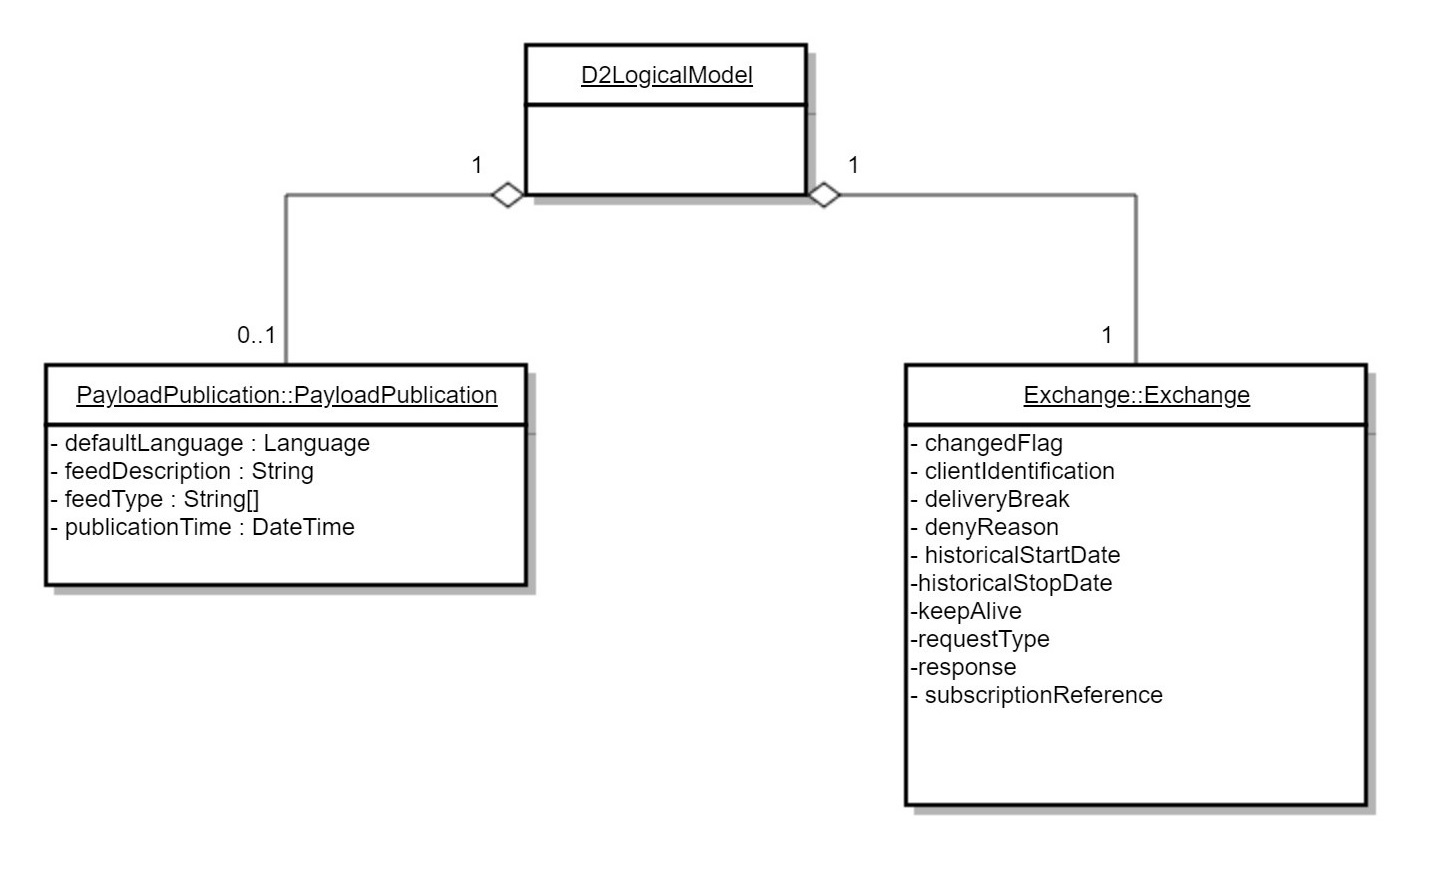
\includegraphics[width=0.6\columnwidth]{images/uml_1}
	\end{center}
	\caption{Distinzione effettuata dallo Standard DATEX II tra metodo di comunicazione (\textit{Exchange}) e formato del Payload (\textit{PayloadPublication})}
	\label{fig:uml_1}
\end{figure}
\begin{figure}
	\begin{center}
		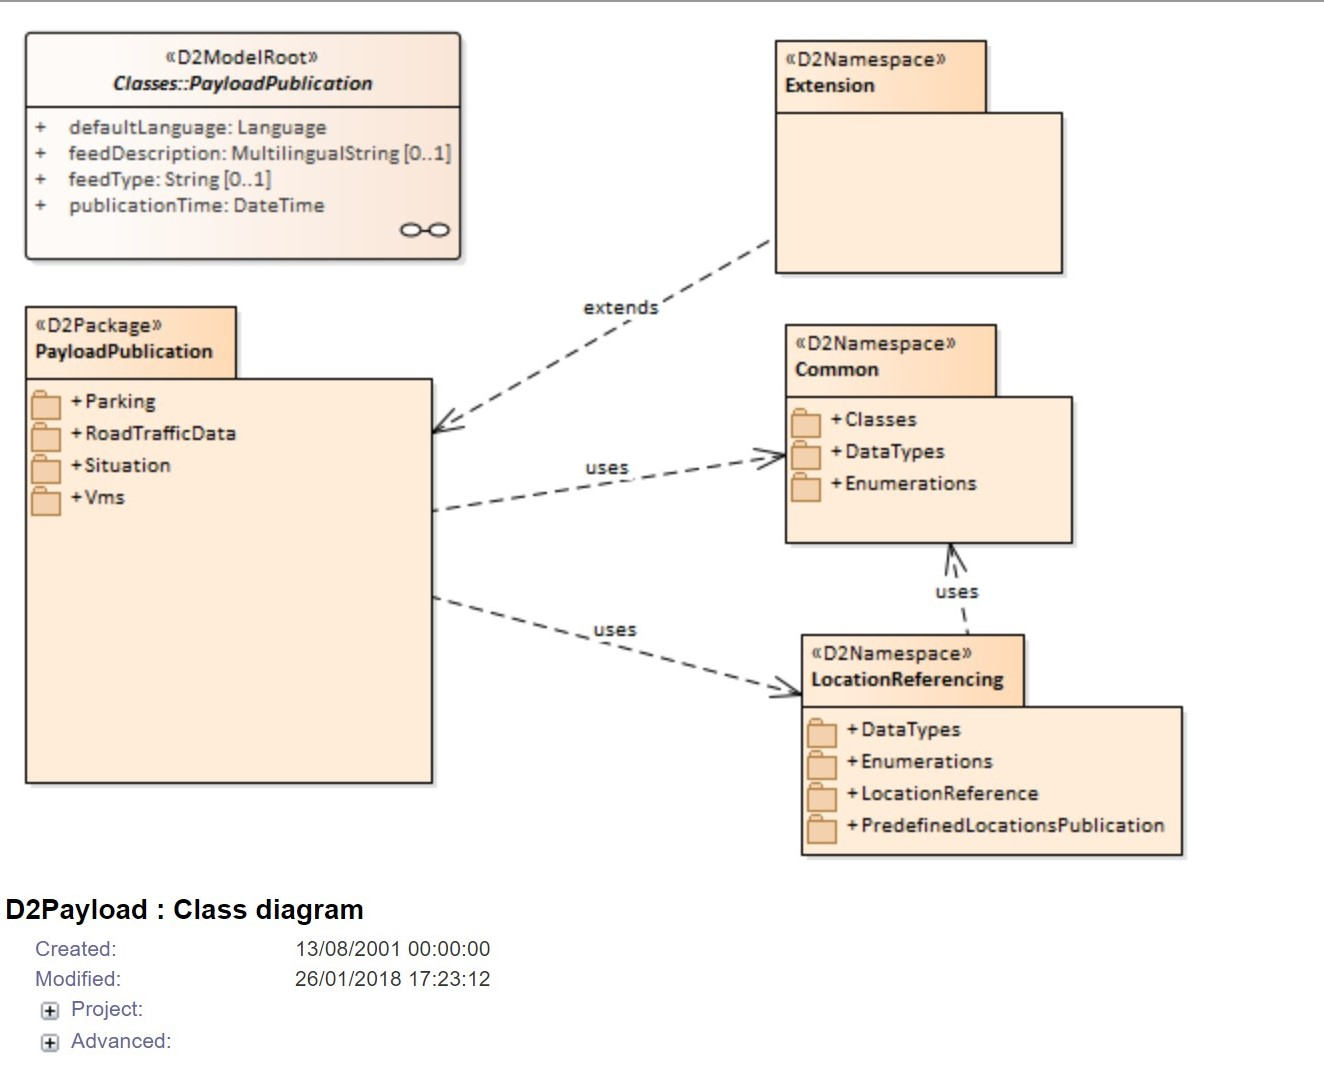
\includegraphics[width=0.6\columnwidth]{images/datexii_publication}
	\end{center}
	\caption{Formato del Payload}
	\label{fig:datexii_publication}
\end{figure}
\begin{figure}
	\begin{center}
		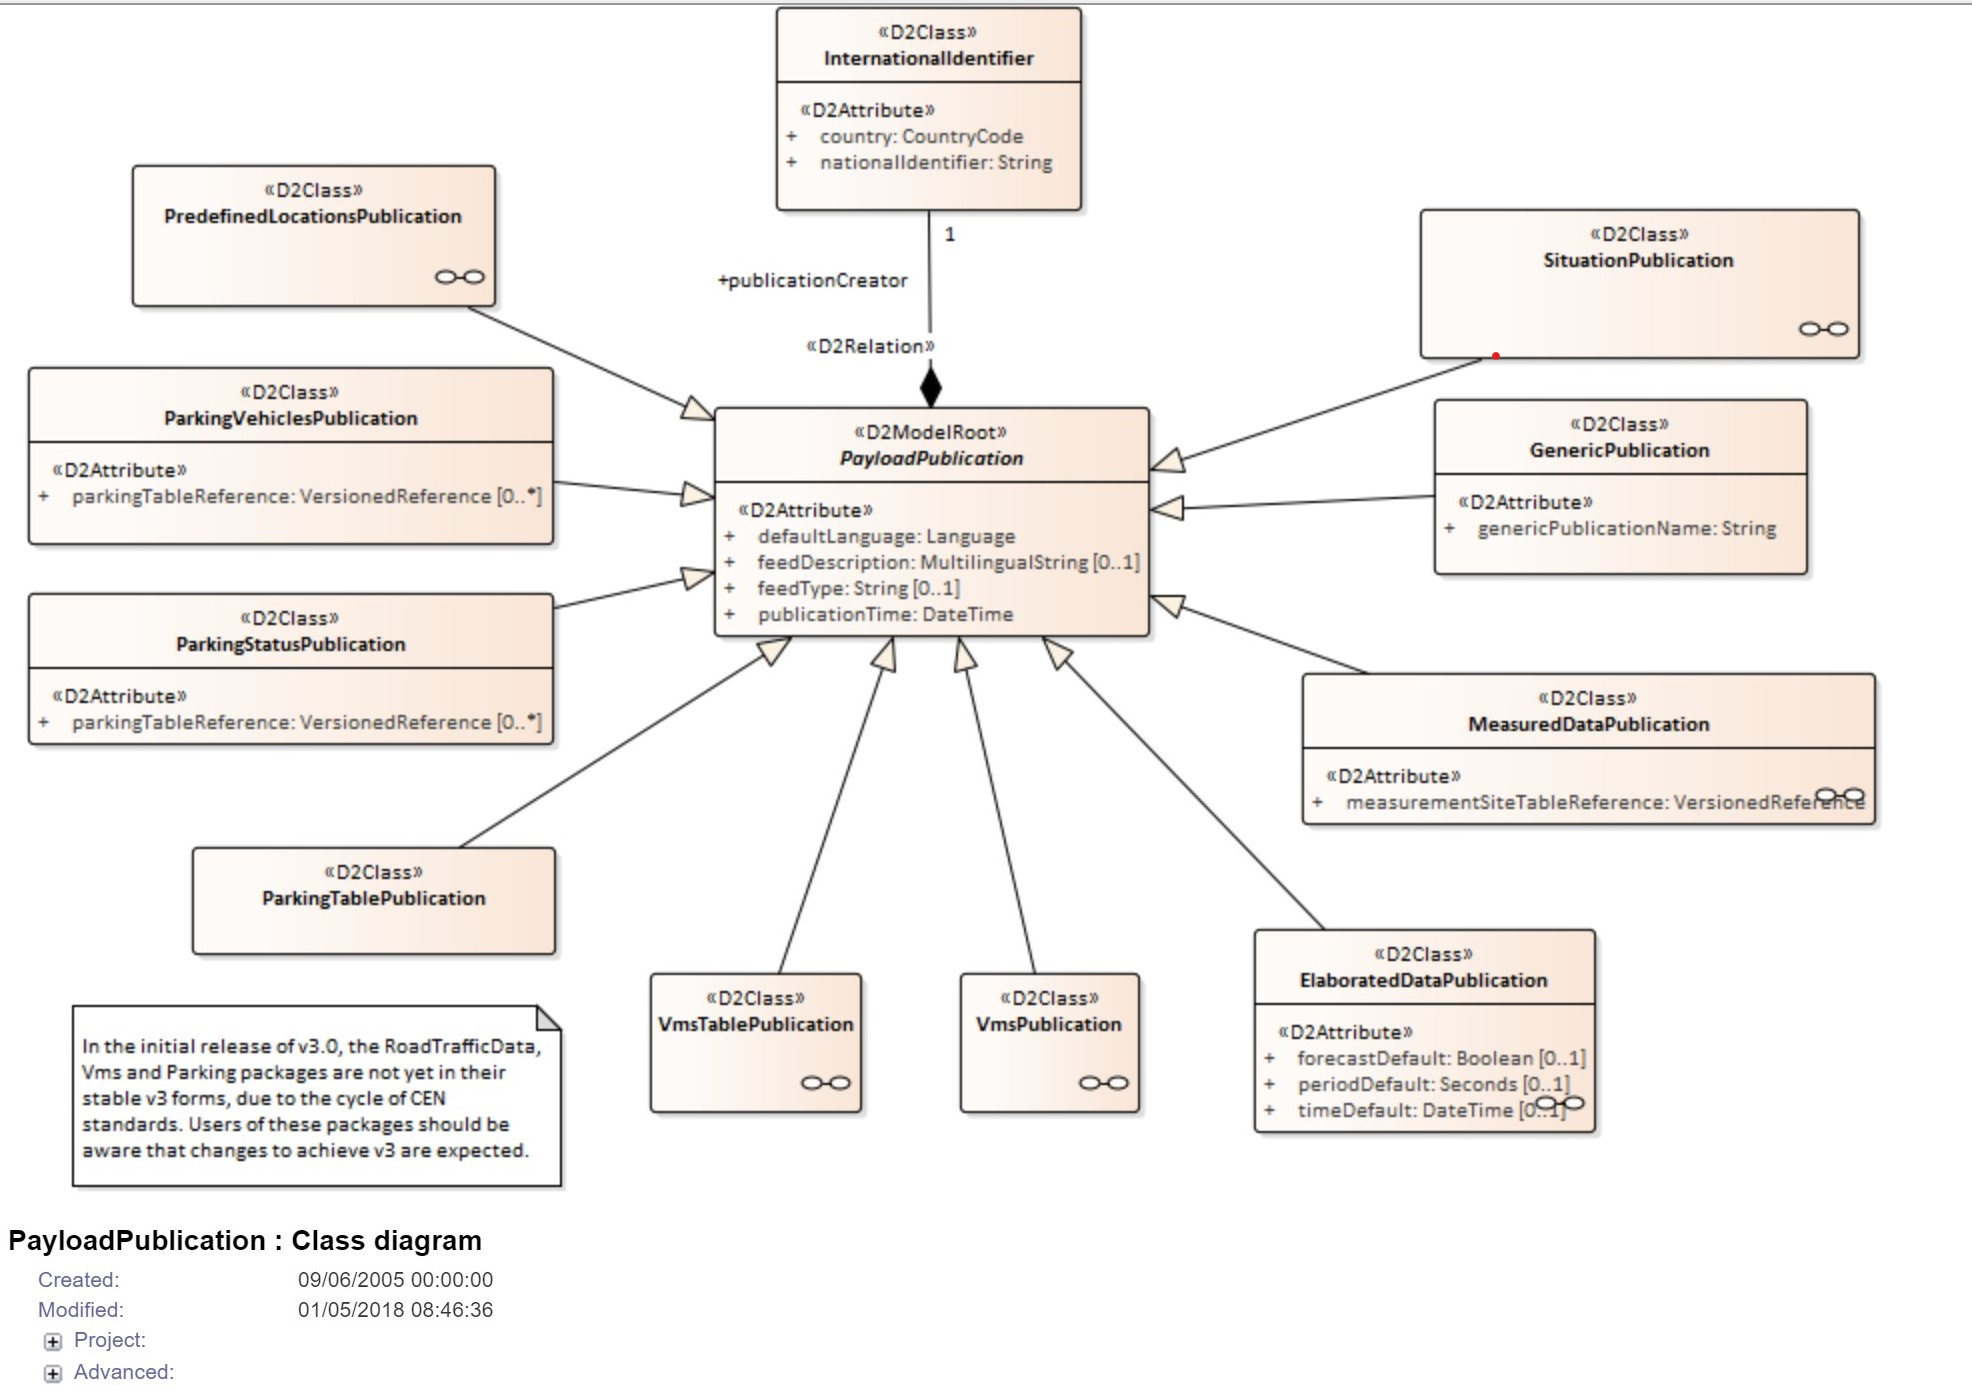
\includegraphics[width=0.75\columnwidth]{images/datexii_publication_detailed}
	\end{center}
	\caption{Formato della Publication}
	\label{fig:datexii_publication_detailed}
\end{figure}
Dalla \autoref{fig:datexii_publication_detailed} è evidente che la classe PayloadPublication sia solo una classe astratta o una interfaccia di classe che viene implementata da altre classi che definiscono tipologie di classi specializzate. Infatti, a conferma di quanto mostrato nella \autoref{sec:publication_base_element}, le Publication possono essere di varie tipologie specializzate a seconda dei dati che trattano.
In funzione dei Requisiti Funzionali in \autoref{tabel:requisiti_software} e dell'idea del sistema nella \autoref{sec:general_idea}, è possibile già filtrare ad alto livello le sole tipologie di publication che è necessario implementare nel sistema.
\begin{figure}
	\begin{center}
		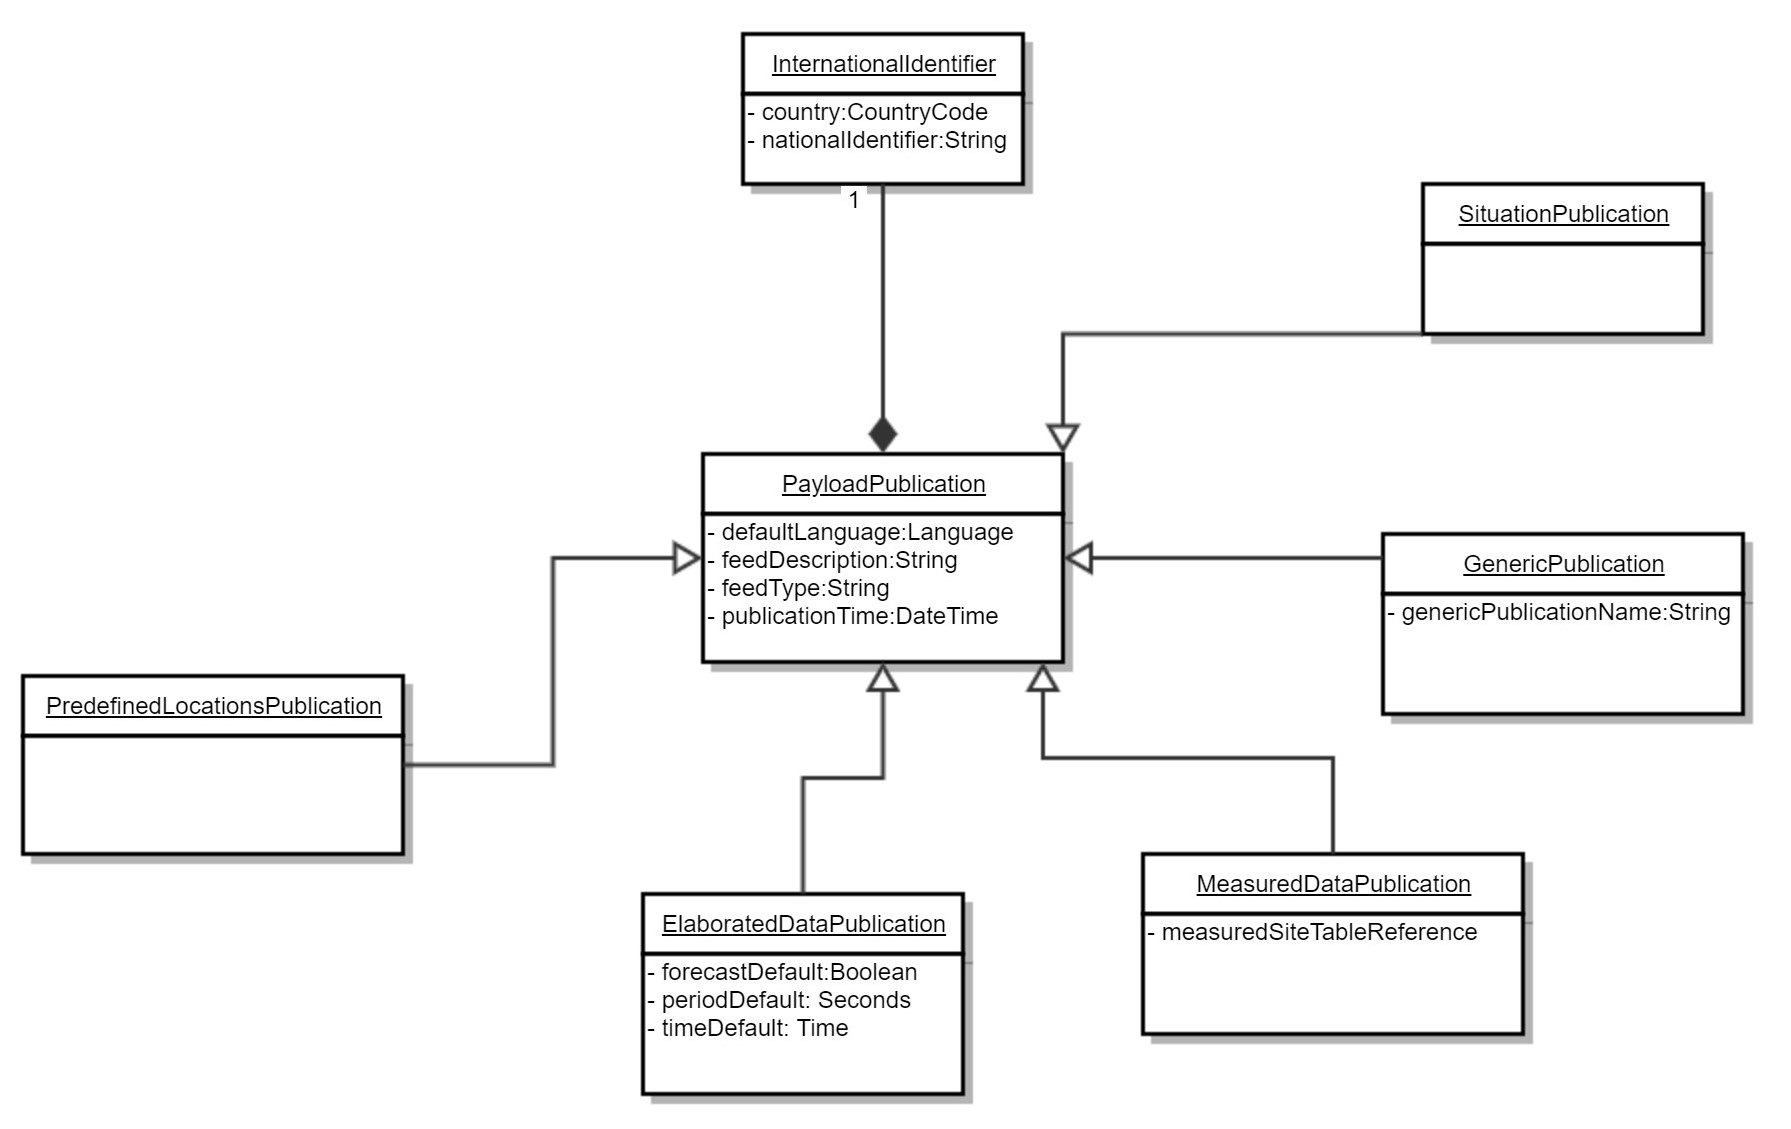
\includegraphics[width=0.8\columnwidth]{images/datexii_publication_implementation}
	\end{center}
	\caption{Implementazione della Publication}
	\label{fig:datexii_publication_implementation}
\end{figure}
Un approccio del tutto simile è stato seguito quindi per tutte le tipologie di Publication che si è ritenuto opportuno implementare. Ovvero, sulla base del diagramma delle classi del protocollo DATEX II, sono state filtrate le sole classi ed attributi necessari a soddisfare i requisiti di \autoref{tabel:requisiti_software}. Il risultato di questo processo è mostrato nell' \autoref{app:a}.

\section{IoT Cloud Platform}
Nella sezione precedente è stato mostrato nei dettagli come procedere all'implementazione del Protocollo DATEX II in un qualsiasi linguaggio di programmazione orientato agli oggetti. In questo modo, si è giunti ad una fase della progettazione del software nella quale i dispositivi che eseguono il sistema, riescono a comunicare tra loro seguendo un Protocollo comune. Sebbene non sia ancora stato definito completamente il contenuto della comunicazione tra due dispositivi (che sarà compito del \autoref{chap:quattro}), è necessario ora progettare una struttura che sia in grado di ricevere questo messaggio, indipendentemente da cosa esso cotenga e di trattarlo opportunamente.\\
E' cioè necessario individuare una Piattaforma Cloud che sia in grado di ricevere i dati provenienti da dispositivi IoT e che sia in grado di conservarli all'interno di opportuni Database, la cui struttura sarà descritta nella \autoref{sec:database}.\\
\begin{figure}
	\begin{center}
		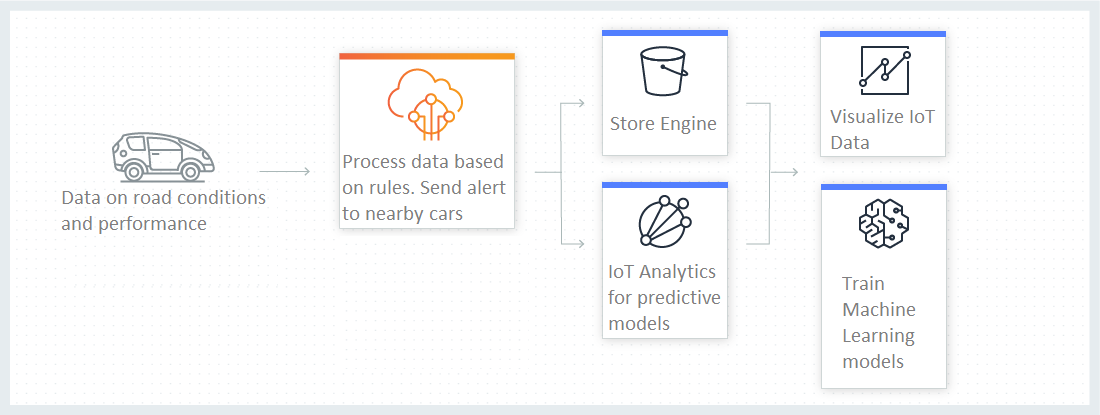
\includegraphics[width=0.9\columnwidth]{images/iot_middleware}
	\end{center}
	\caption{Schema della componente che si vuole implementare in questa sezione vista nel progetto completo}
	\label{fig:iot_middleware}
\end{figure}
Dal momento che il panorama attuale offre numerosi servizi che possano assolvere a questo compito, si valutino ora i requisiti che il Middleware IoT deve avere per l'implementazione del sistema descritto nella \autoref{sec:general_idea} e, sulla base di questi requisiti, si effettuerà un confronto tra le possibili soluzioni.\\
I requisiti mostrati nella \autoref{tabel:requisiti_middleware} vanno ad aggiungersi a quelli elencati nella \autoref{tabel:requisiti_software} concludendo in questo modo la redazione dell' Analisi dei Requisiti prevista nel Processo Unificato.\\\\
\begin{longtable}{|m{2cm}|m{12cm}|}
	\hline
	\textbf{Requisito} & \textbf{Descizione} \\
	\hline
	\textbf{M1} &   Il Middleware IoT dovrà prevedere un sistema per la registrazione di nuovi utenti \\
	\hline
	\textbf{M2} &   Il Middleware IoT dovrà consentire l'accesso ai soli utenti registrati, instaurando con essi una connessione sicura \\
	\hline
	\textbf{M3} &   Il Middleware IoT dovrà consentire di assegnare diversi ruoli a diversi utenti con diverse permission \\
	\hline
	\textbf{M4} &   Il Middleware IoT deve trattare diversamente i dati provenienti da diverse località geografiche \\
	\hline
	\textbf{M5} &   Il Middleware IoT deve stabilire una comunicazione con un database di tipo SQL/NoSQL per il salvataggio dei dati \\
	\hline
	\textbf{M6} &   Il Middleware IoT dovrà  stabilire una comunicazione di tipo publisher/subscriber con uno o più dispositivi IoT\\
	\hline
	\textbf{M7} &   Il Middleware IoT dovrà essere altamente scalabile per supportare un numero sempre crescente di dispositivi \\
	\hline
	\textbf{M8} &   Il Middleware IoT dovrà consentire la comunicazione con sistemi per la visualizzazione ed analisi dei dati \\
	\hline
	\textbf{M9} &   Il Middleware IoT dovrà implementare il protocollo DATEX II \\
	\hline
	\textbf{M10} &   Il Middleware IoT dovrà supportare diversi protocolli per la comunicazione (MQTT, HTTP, AMQP, etc) per garantire la comunicazione con dispositivi eterogenei \\
	\hline
	\caption{Analisi dei requisiti che la IoT Cloud Platform deve supportare}
	\label{tabel:requisiti_middleware}
\end{longtable}
Le piattaforme che sono state individuate come possibili Cloud Platforms adatte allo scopo sono:
\begin{itemize}
	\item \textbf{AWS IoT Core: } \url{https://aws.amazon.com/it/iot-core/}
	\item \textbf{Azure IoT Lab: } \url{https://docs.microsoft.com/en-us/azure/iot-hub/about-iot-hub}
	\item \textbf{FIWARE: } \url{https://www.fiware.org/about-us/}
\end{itemize}
Le soluzioni identificate, non rappresentano assolutamente l'insieme di tutte le soluzioni possibili per le Cloud Platform, ma solo di quelle ritenute più adatte allo scopo della progettazione del sistema.\\
Di seguito viene proposto un confronto tra le diverse soluzioni elencate sulla base dei requisiti di \autoref{tabel:requisiti_middleware}. Le informazioni sulla base delle quali è stato effettuato questo confronto sono state raccolte dai siti Web di ciascuna soluzione e si intendono riferiti alla alla data della seduta di laurea alla quale questo elaborato si riferisce.\\
\begin{table}
	\centering
	\begin{tabular}{|>{\centering\arraybackslash}m{2.5cm}|>{\centering\arraybackslash}m{4cm}|>{\centering\arraybackslash}m{4cm}|>{\centering\arraybackslash}m{4cm}|}
		\hline
		\textbf{Requisito} & \textbf{AWS IoT Core} & \textbf{Azure IoT Lab} & \textbf{Fiware} \\
		\hline
		\textbf{M1} &  \textcolor{green}{\checkmark} &   \textcolor{green}{\checkmark} &   \textcolor{green}{\checkmark} \\
		\hline
		\textbf{M2} &  \textcolor{green}{\checkmark} &   \textcolor{green}{\checkmark} &   \textcolor{green}{\checkmark} \\
		\hline
		\textbf{M3} &  \textcolor{green}{\checkmark} &   \textcolor{green}{\checkmark} &   \textcolor{red}{$\times$} \\
		\hline
		\textbf{M4} &  \textcolor{green}{\checkmark} &   \textcolor{red}{$\times$} &   \textcolor{green}{\checkmark} \\
		\hline
		\textbf{M5} &  \textcolor{green}{\checkmark} &   \textcolor{green}{\checkmark} &   \textcolor{orange}{Not Implemented} \\
		\hline
		\textbf{M6} &  \textcolor{green}{\checkmark} &   \textcolor{green}{\checkmark} &   \textcolor{orange}{Not Implemented} \\
		\hline
		\textbf{M7} &  \textcolor{green}{\checkmark} &   \textcolor{green}{\checkmark} &   \textcolor{green}{\checkmark} \\
		\hline
		\textbf{M8} &  \textcolor{green}{\checkmark} &   \textcolor{green}{\checkmark} &   \textcolor{orange}{Not Implemented} \\
		\hline
		\textbf{M9} &  \textcolor{green}{\checkmark} &   \textcolor{green}{\checkmark} &   \textcolor{green}{\checkmark} \\
		\hline
		\textbf{M10} &  \textcolor{green}{\checkmark} &   \textcolor{green}{\checkmark} &   \textcolor{green}{\checkmark} \\
		\hline
	\end{tabular}	
	\caption{Confronto tra Cloud Platforms}
	\label{tabel:platform_comparison}
\end{table}
Si noti come, la soluzione proposta da Fiware sia particolarmente interessante in quanto offre una piattaforma open source che quindi può essere adattata alle particolari necessità. Tale soluzione, può essere ritenuta infatti molto promettente per quelle compagnie che vogliano progettare su misura la Cloud Platform ed adattarla alle proprie necessità in modo da avere dei migliori rendimenti prestazionali. Infatti, una soluzione personalizzata, potrebbe offrire prestazioni migliori di soluzioni generali come quelle offerte da AWS ed Azure.\\
Tuttavia, per il dominio di questo lavoro di tesi, la soluzione ideale è quella di sfruttare piattaforme cloud generiche per la raccolta dei dati. In questo modo, si godrà di un ecosistema di servizi ampiamente documentato e ben interfacciato. Infatti, ecosistemi come AWS ed Azure offrono diversi servizi e diverse applicazioni anche al di fuori del dominio dell'IoT. Queste possono essere ad esempio relative ad analisi dei dati, raccolta e storaggio dei dati, servizi di autenticazione e piattaforme di calcolo e machine learning. Tutti questi servizi, sono facilmente utilizzabili e possono facilmente comunicare tra di loro scambiandosi in maniera automatica i dati di cui necessitano. In piattaforme open source, invece, è necessario sviluppare ed interfacciare ciacuno di questi servizi, richiedendo di fatto una mole di lavoro estremamente maggiore.\\
Questa scelta è anche da considerarsi adatta per coloro i quali si interfacciano per la prima volta con una piattaforma cloud in quanto numerosi sono i corsi e le documentazioni offerte da AWS ed Azure.\\
Considerato infine che le funzioni offerte da AWS ben soddisfano i requisiti della \autoref{tabel:requisiti_middleware}, si è scelto di utilizzare questa piattaforma come Middleware IoT che si occuperà della raccolta, condivisione e salvataggio dei dati.

\subsection{AWS IoT Core Overview}
\label{sec:iot_core}
Amazon Web Services IoT Core è una piattaforma cloud che consente a dispostivi connessi di interagire tra loro e con altre applicazioni nel cloud. Inoltre, IoT Core, si interfaccia con tutti gli altri servizi offerti da AWS per il cloud computing and analysis. Ad esempio sarà semplice interfacciare i dati raccolti da IoT core con altri servizi quali:
\begin{itemize}
	\item \textbf{Amazon S3} per la memorizzazione dei dati in Database SQL
	\item \textbf{Amazon DynamoDB} per la memorizzazione dei dati in Database NoSQL
	\item \textbf{Amazon Kinesis ed Amazon QuickSight} per la visualizzazione ed analisi dei dati
	\item \textbf{TensorFlow in AWS} per l'elaborazione dei dati raccolti con tecniche di Machine Learning
\end{itemize}
\begin{figure}
	\begin{center}
		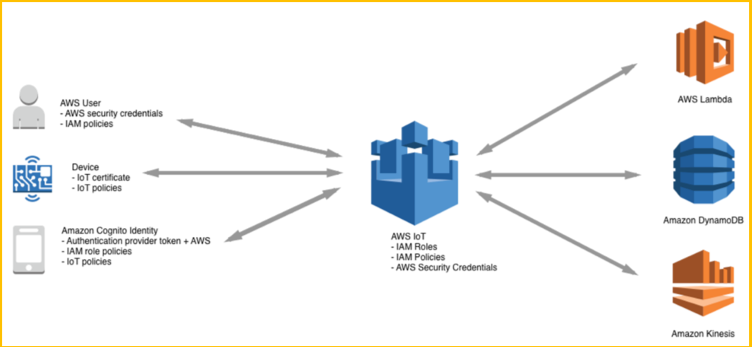
\includegraphics[width=0.9\columnwidth]{images/aws_iot_core}
	\end{center}
	\caption{Capacità di interfacciamento della piattaforma IoT Core con gli altri servizi dell'ecosistema AWS}
	\label{fig:aws_iot_core}
\end{figure}
\begin{figure}
	\begin{center}
		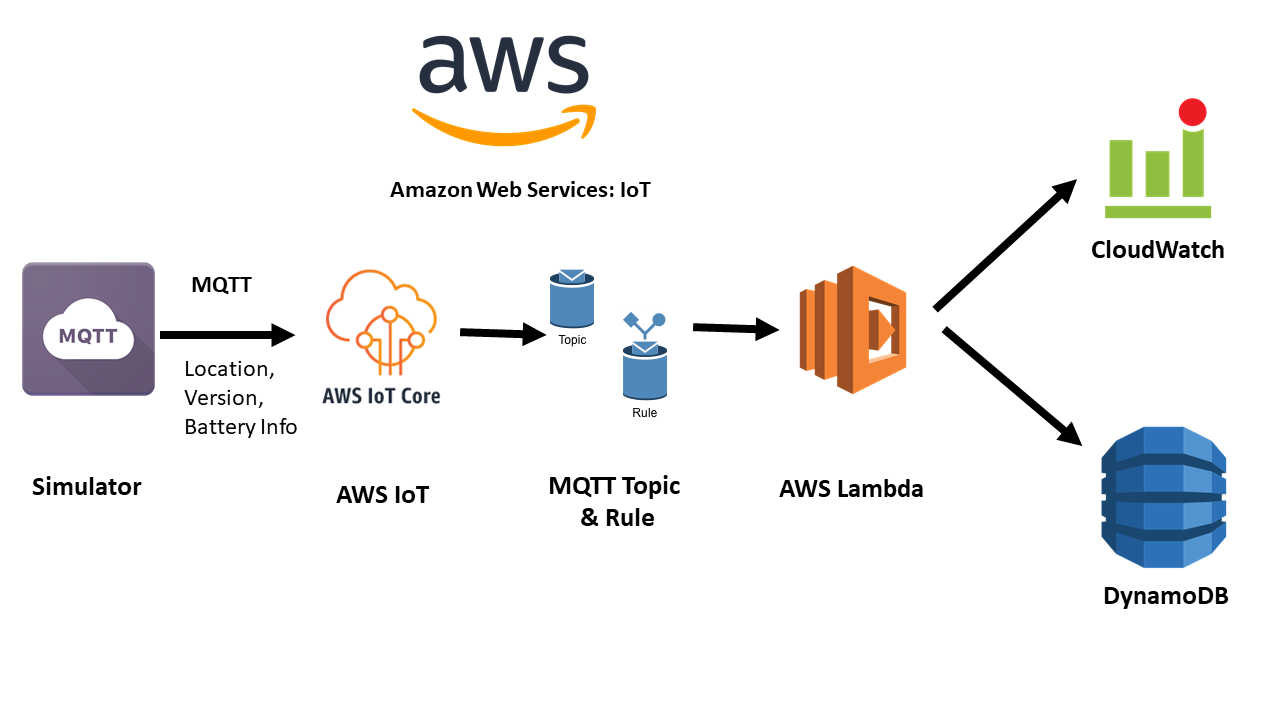
\includegraphics[width=0.9\columnwidth]{images/aws_iot_core_2}
	\end{center}
	\caption{Esempi di utilizzo della piattaforma IoT Core combinata con altri servizi dell'ecosistema AWS}
	\label{fig:aws_iot_core_2}
\end{figure}
Alcune tra le comuni applicazioni IoT raccolgono ed elaborano dati di telemetria dai dispositivi oppure permettono agli utenti di controllare un dispositivo in remoto. I dispositivi segnalano il proprio stato pubblicando messaggi, in formato JSON, in argomenti MQTT. Ogni argomento MQTT ha un nome gerarchico che identifica il dispositivo il cui stato è in fase di aggiornamento. Quando vengono pubblicati in un argomento MQTT, i messaggi vengono inviati al broker di messaggi MQTT AWS IoT, responsabile dell'invio di tutti i messaggi pubblicati in un argomento MQTT a tutti i client che hanno sottoscritto l'argomento.\\
La comunicazione tra un dispositivo e AWS IoT è protetta dai certificati X.509.\\
AWS IoT è in grado di generare un certificato per l'accesso in maniera automatica oppure creato manualmente . In entrambi i
casi, il certificato deve essere registrato e attivato su AWS IoT e quindi copiato nel dispositivo. Quando il dispositivo comunica con AWS IoT, presenta il certificato a AWS IoT come credenziale.\\
\begin{figure}
	\begin{center}
		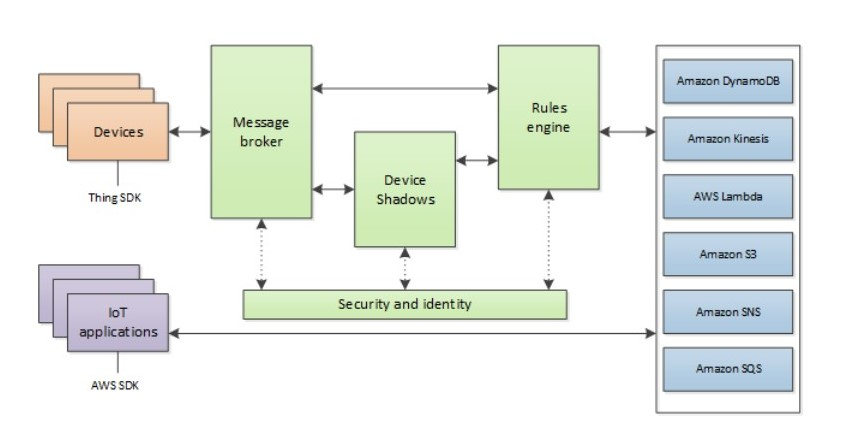
\includegraphics[width=0.9\columnwidth]{images/aws_structure}
	\end{center}
	\caption{Struttura della comunicazione}
	\label{fig:aws_structure}
\end{figure}


\subsubsection{Authentication}
AWS IoT Core offre autenticazione reciproca e crittografia in tutti i punti di connessione, perciò non si verificherà mai alcuno scambio di dati tra dispositivi e AWS IoT Core senza accertamenti di identità. AWS IoT Core supporta il metodo di autenticazione di AWS (denominato "SigV4"), l'autenticazione basata su certificato X.509 e l'autenticazione basata su token creati dal cliente (mediante autorizzazioni ad hoc). Le connessioni che impiegano il protocollo HTTP possono usare tutti i metodi disponibili, mentre le connessioni MQTT usano l'autenticazione basata su certificato e le connessioni WebSockets possono usare SigV4 o autorizzazioni ad hoc. È possibile mappare policy per ciascun certificato per autorizzare l'accesso di dispositivi e applicazioni e revocare l'accesso in qualsiasi momento senza toccare il dispositivo.

\begin{figure}
	\begin{center}
		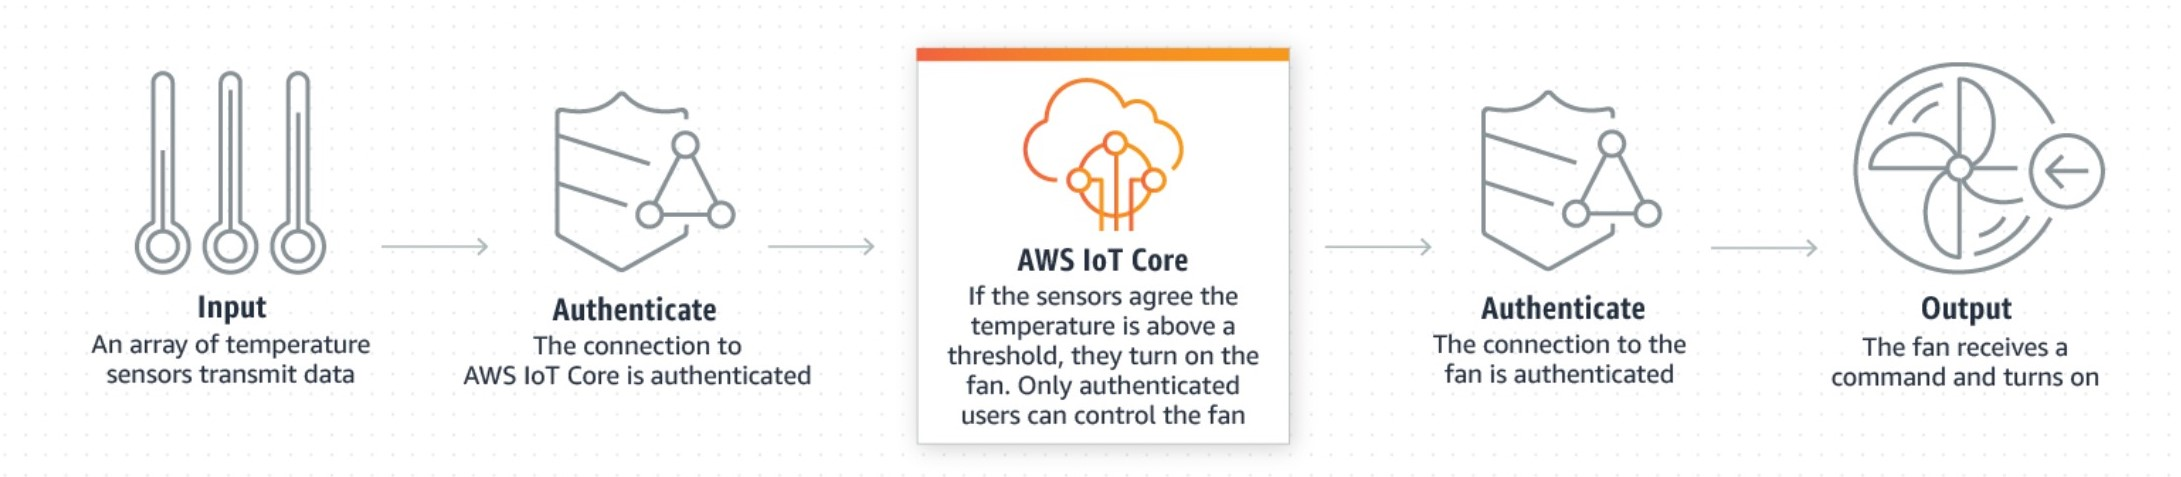
\includegraphics[width=0.9\columnwidth]{images/aws_auth}
	\end{center}
	\caption{Processo di autenticazione implementato in ogni punto della connessione}
	\label{fig:aws_auth}
\end{figure}

È possibile creare, distribuire e gestire certificati e policy per i dispositivi tramite la console o l'API. I certificati dei dispositivi possono essere assegnati, attivati e associati con le policy IoT corrispondenti configurate tramite AWS IoT Core. In questo modo sarà possibile revocare istantaneamente l'accesso per singoli dispositivi. AWS IoT Core supporta inoltre le connessioni dalle app per dispositivi mobili degli utenti tramite Amazon Cognito, che crea un identificatore univoco e recupera credenziali temporanee di AWS con privilegi limitati. AWS IoT Core fornisce inoltre credenziali AWS temporanee quando un dispositivo si autentica con un certificato X.509, per facilitare al dispositivo l'accesso ad altri servizi AWS, ad esempio DynamoDB o S3.

\subsubsection{Shadow dei Dispositivi}
Con AWS IoT Core è possibile creare versioni virtuali e persistenti dei dispositivi, chiamate "shadow" dei dispositivi (copia digitale del dispositivo), che includono l'ultimo stato noto del dispositivo, consentendo ad applicazioni e altri dispositivi di leggerne i messaggi e interagire con esso. La shadow dei dispositivi conserva l'ultimo stato noto e lo stato futuro impostato per ciascun dispositivo anche quando è offline. Per recuperare l'ultimo stato noto di un dispositivo o impostare uno stato futuro, è possibile usare l'API o il motore di regole.

La shadow dei dispositivi semplifica la creazione di applicazioni che interagiscono con i dispositivi perché fornisce sempre API REST disponibili. Inoltre, le applicazioni possono impostare uno stato futuro per un dispositivo indipendentemente dal suo stato corrente. AWS IoT Core confronterà lo stato futuro con l'ultimo stato noto e imporrà al dispositivo di aggiornarsi.

\subsection{AWS IoT Core Development}
\label{subsec:aws_dev}
Dopo aver visto le main features della cloud platform AWS IoT Core, si progettino ora gli step implementativi da seguire al fine di integrare correttamente il sistema progettato nelle precedenti sezioni con la cloud platform.
A tal scopo, sarà necessario seguire la documentazione messa a disposizione da AWS IoT Core per ottenere delle linee guida più dettagliate sui passi da seguire \url{https://docs.aws.amazon.com/it_it/iot/latest/developerguide/iot-dg.pdf}.\\
Gli step implementativi progettati in questa sezione si intendono riferiti ad una qualsiasi implementazione della cloud platform in un qualsiasi linguaggio di programmazione e per un qualsiasi progetto. I dettagli implementativi relativi al software sviluppato in questo lavoro di tesi, sarnno invece mostrati nel \autoref{chap:quattro}.\\
\begin{enumerate}
	\item Accesso alla Console AWS IoT Core e creazione di un nuovo account
	\item Registrazione e Configurazione di un nuovo dispositivo come copia digitale (o shadow) di un dispositivo reale
	\item Configurazione della comunicazione con il protocollo MQTT
	\item Utilizzo dell' SDK messa a sisposizione da AWS per l'abilitazione dei dispositivi IoT alla comunicazione con il Broker centrale.
\end{enumerate}

\subsubsection{Accesso alla Console AWS IoT Core}
Al fine di poter utilizzare i servizi offerti da AWS è necessario prima seguire un processo di registrazione di un nuovo account presso \url{https://aws.amazon.com/it/} e quindi seguire la procedura guidata per la Creazione di un Nuovo Account. \\
Una volta completata la procedura di resistrazione è quindi possibile accedere alla piattaforma IoT Core ed iniziare a creare un nuovo dispositivo.
\begin{figure}
	\begin{center}
		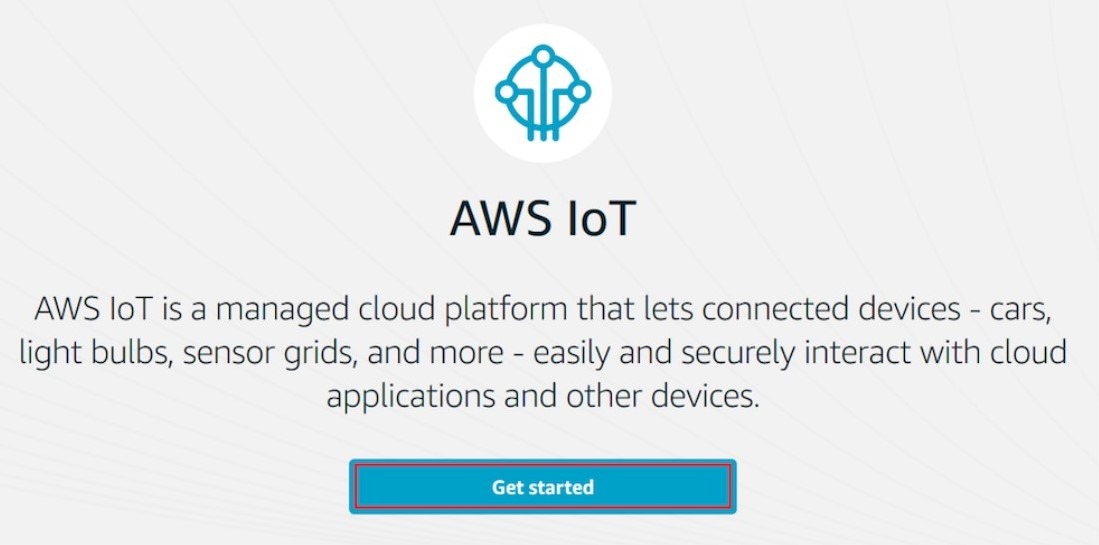
\includegraphics[width=0.9\columnwidth]{images/_1}
	\end{center}
	\caption{Primo accesso alla piattaforma IoT Core}
	\label{fig:_1}
\end{figure}

\subsubsection{Registrazione e Configurazione di un nuovo dispositivo}
I dispositivi connessi a AWS IoT sono rappresentati da oggetti IoT nel registro AWS IoT. Questo registro permette di tenere traccia di un record di tutti i dispositivi registrati nell'account AWS IoT in modo da poter assegnare a ciascun dispositivo diversi ruoli e quindi diverse permission.\\
Si rende quindi necessario creare ora una copia digitale di ogni dispositivo abilitato alla comunicazione con AWS IoT Core. In realtà, per evitare di creare un numero infinitamente grande di dispositivi diversi, un'approccio più adatto è quello di creare delle macro-categorie di oggetti che possono collegarsi alla piattaforma cloud. \\
Volendo, in questo lavoro di tes,i abilitare la comunicazione tra i soli smartphone con sistema operativo Android ed il Middleware IoT, si crei un unico oggetto denominato \textbf{Android\_Device} che si riferisca quindi a tutti i dispositivi Android che si collegano al Middleware. Allo stesso modo, è possibile creare una qualsiasi categoria di oggetti come ad esempio: \textbf{iOS\_Device}, \textbf{Windows\_Device}, \textbf{VMS\_Device}, etc.\\
La procedura per la creazione di un nuovo oggetto è descritta nei dettagli in \url{https://docs.aws.amazon.com/it_it/iot/latest/developerguide/iot-dg.pdf} ed il risultato finale sarà la comparsa di un nuovo prototipo di oggetto \textit{shadow} all'interno del IoT Core.
\begin{figure}
	\begin{center}
		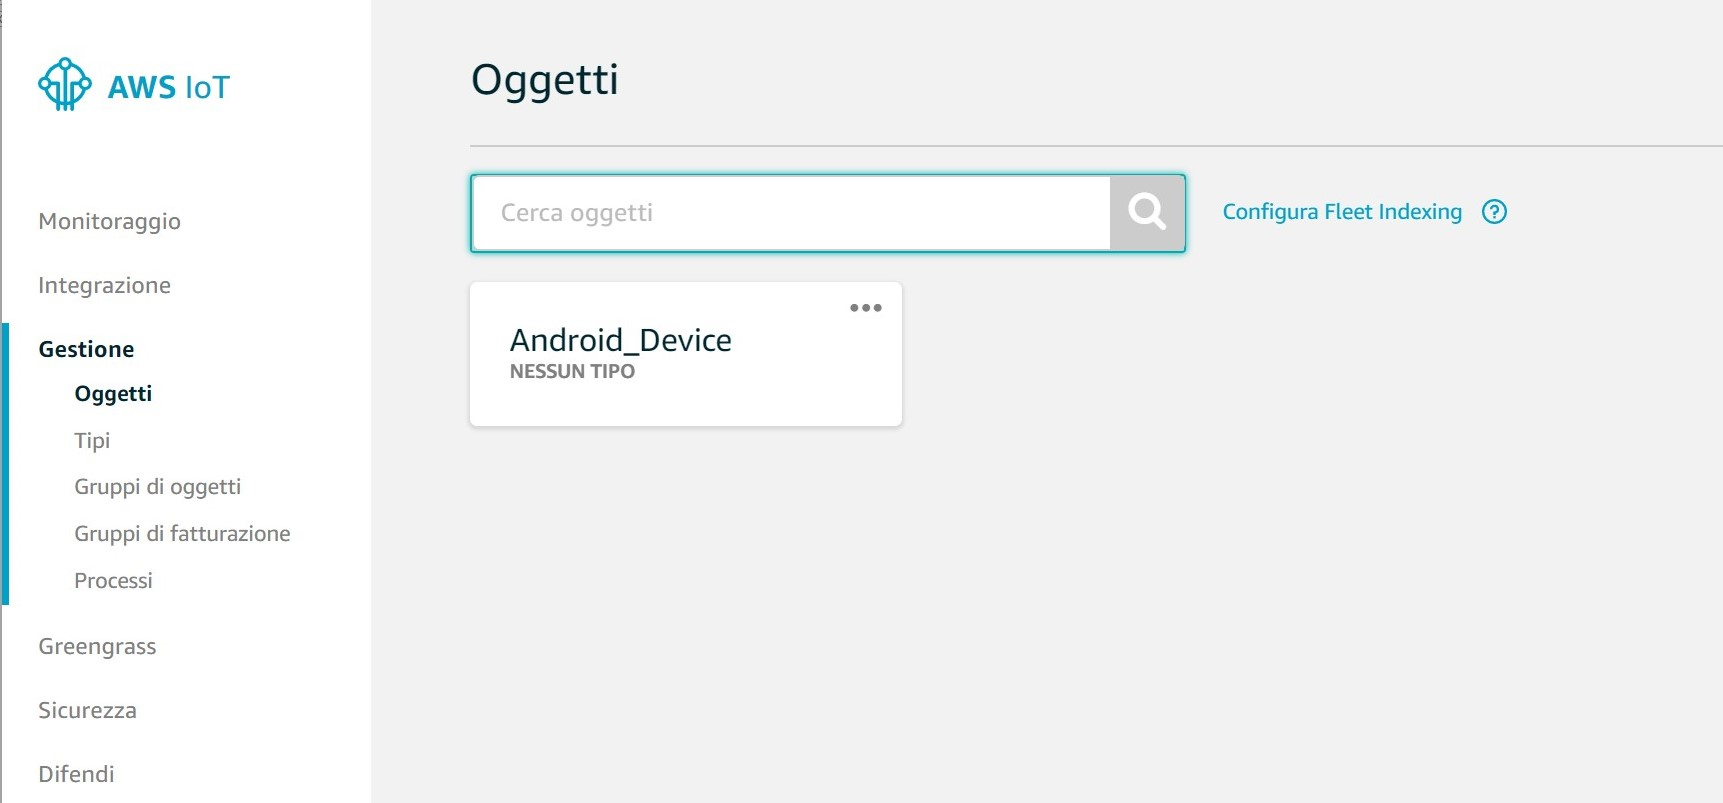
\includegraphics[width=0.9\columnwidth]{images/_2}
	\end{center}
	\caption{Creazione di un nuovo oggetto nella pagina principale di AWS IoT Core.}
	\label{fig:_2}
\end{figure}
Una volta creato, il nuovo dispositivo ha bisogno che vi siano assegnate delle perimission e quindi una Policy per poter comunicare con la Cloud Platform. AWS prevede infatti la possibilità di poter assegnare diverse Policy a diversi dispositivi che quindi avranno accesso a diverse componenti e servizi della Cloud Platform. Questo è fatto per garantire alti livelli di sicurezza e di gestione degli accessi a particolari servizi. Ad esempio, in questo modo potrebbero essere offerte alcune funzionalità a tutti i dispositivi, ed altre funzionalità premium ai soli dispositivi con un diverso piano tariffario.\\
Per lo scope di questo lavoro di tesi, la Policy che sarà assegnata al dispositivo appena creato (\textbf{Android\_Device}), sarà quella che gli consentirà di eseguire tutte le operazioni AWS IoT su tutte le risorse
AWS IoT. Queste impostazioni sono adatte ad un ambiente di sviluppo per facilitare il debugging ma sono ovviamente eccessivamente permissive ed è quindi opportuno restringere l'ambito delle autorizzazioni a quelle richieste dal dispositivo in un ambiente di produzione.\\
Anche in questo caso, per evitare ridondanze, si rimanda alla procedura per la creazione ed assegnazione di una nuova Policy ad un oggetto shadow creato, si rimanda alla documentazione ufficiale.

\subsubsection{Configurazione della Comunicazione}
\label{subsubsec:com}
A questo punto della configurazione, è possibile testare la comunicazione tra il Client (oggetto appena creato ed al quale è stata associata una Policy) ed il Server (IoT Core). \\
AWS IoT Core, consente inoltre di stabilire la comunicazione Client / Server seguendo diversi protocolli di comunicazione tra i quali MQTT ed HTTP che possono essere interscambiati a piacere.\\
In riferimento al \autoref{chap:introduzione} dove si era fatto un confronto tra i due protocolli e sui vantaggi dell'utilizzo di uno piuttosto che dell'altro, era evidente come il protocollo MQTT fossepiù efficiente in termini di consumo energetico e nella capacità comuputazionale richiesta. Pertanto, vista la frammentazione del mondo Android in termini di versioni del sistema operativo implementate ed anche in termini di obsolescenza dei dispositivi, si ritiene più adatto l'utilizzo del protocollo MQTT per stabilire una comunicazione tra il Client Android ed il server AWS.\\
\begin{figure}
	\begin{center}
		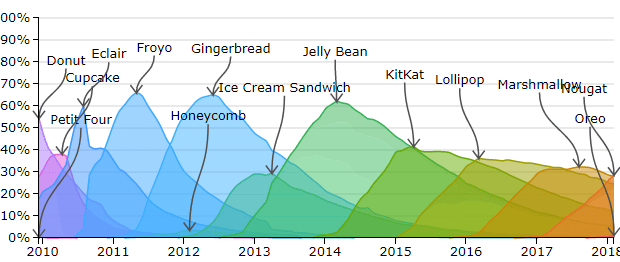
\includegraphics[width=0.9\columnwidth]{images/android_fragmentation}
	\end{center}
	\caption{Panorama della frammentazione nella distribuzione delle versioni del sistema operativo Android}
	\label{fig:android_fragmentation}
\end{figure}
Si testi quindi ora la comunicazione di tipo Publish - Subscribe tra il Client ed il Server (\autoref{sec:MQTT_protocol}).\\
Un dispositivo pubblicherà dei messaggi all'interno di un Topic ed è possibile impostare il Server IoT Core in modo da essere in ascolto sullo stesso Topic, caratterizzato cioè dallo stesso nome.\\
Nella sezione Test della console IoT Core, sono presenti due sottosezioni : \textbf{Pubblicare}  e \textbf{Sottoscrivere}.
\begin{figure}
	\begin{center}
		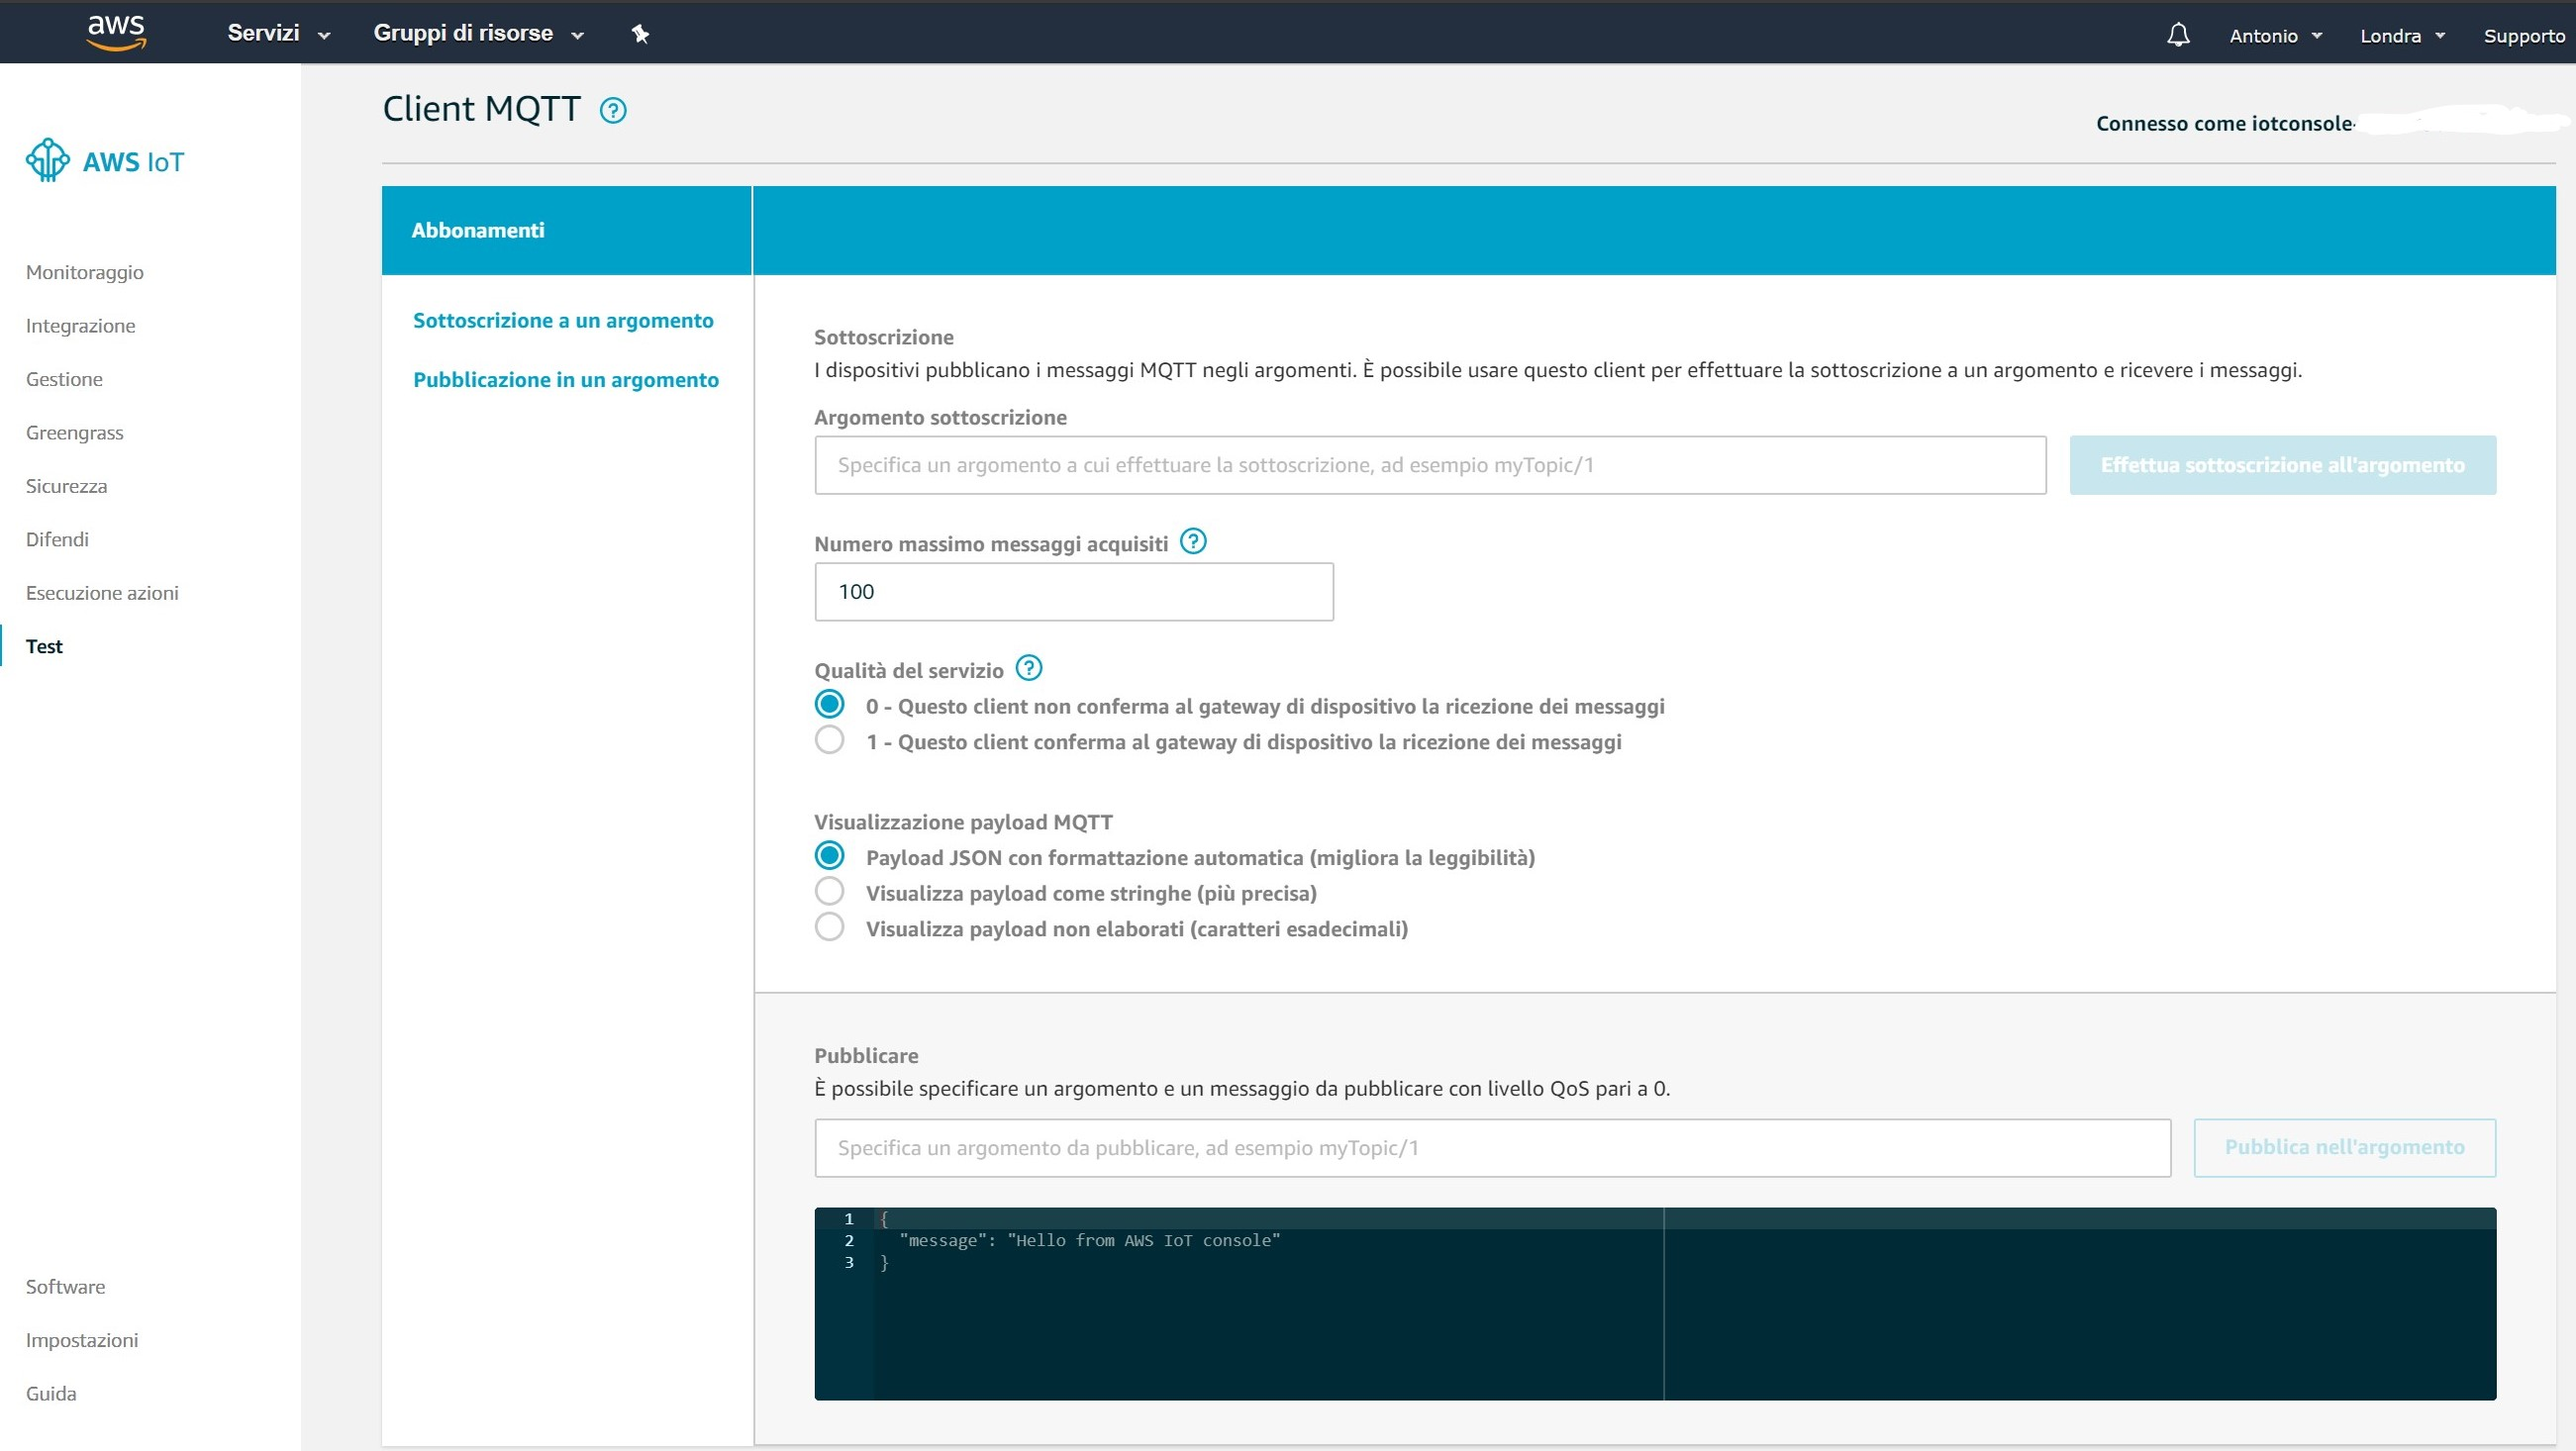
\includegraphics[width=1\columnwidth]{images/_3}
	\end{center}
	\caption{Panoramica della schermata Test}
	\label{fig:_3}
\end{figure}
Nella sezione \textbf{Sottoscrivere}, va specificato il nome del Topic al quale registrarsi o meglio sul quale restare in ascolto. Questo Topic sarà caratterizzato dsllo stesso nome del Topic sul quale il dispositivo comunicherà o meglio pubblicherà.
\begin{figure}
	\begin{center}
		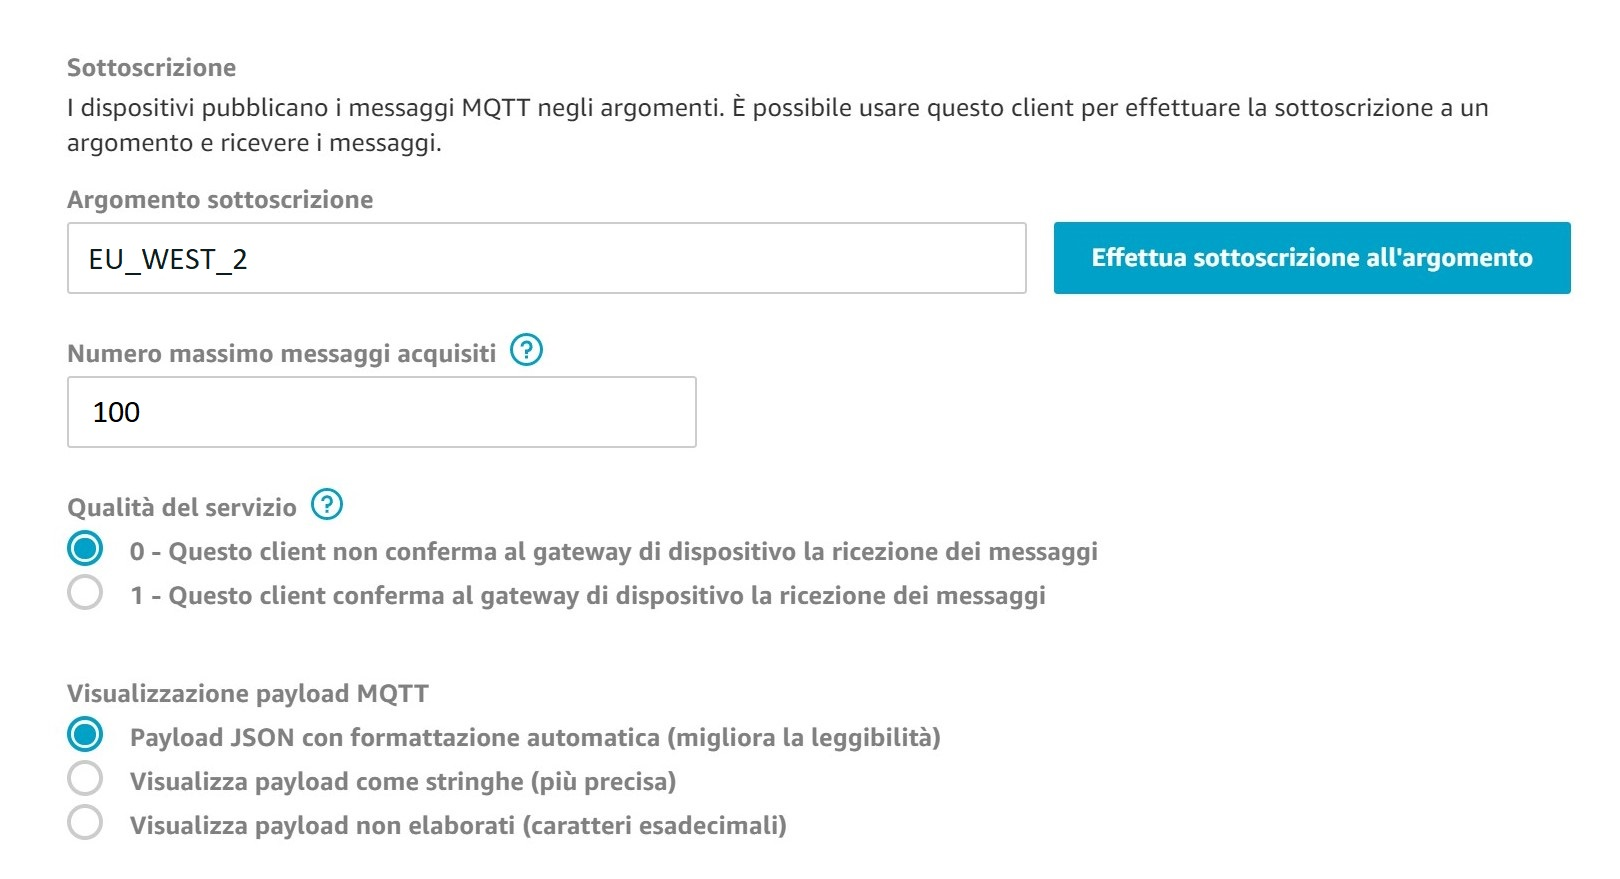
\includegraphics[width=0.8\columnwidth]{images/_4}
	\end{center}
	\caption{Sottoscrizione al Topic \textbf{EU\_WEST\_2}}
	\label{fig:_4}
\end{figure}
Infine, per simulare il comportamento di un dispositivo IoT che pubblichi un messaggio all'interno di un argomento, si pubblichi un messaggio nella sezione \textbf{Pubblicare} che faccia riferimento allo stesso topic sul quale si è in ascolto.
\begin{figure}
	\begin{center}
		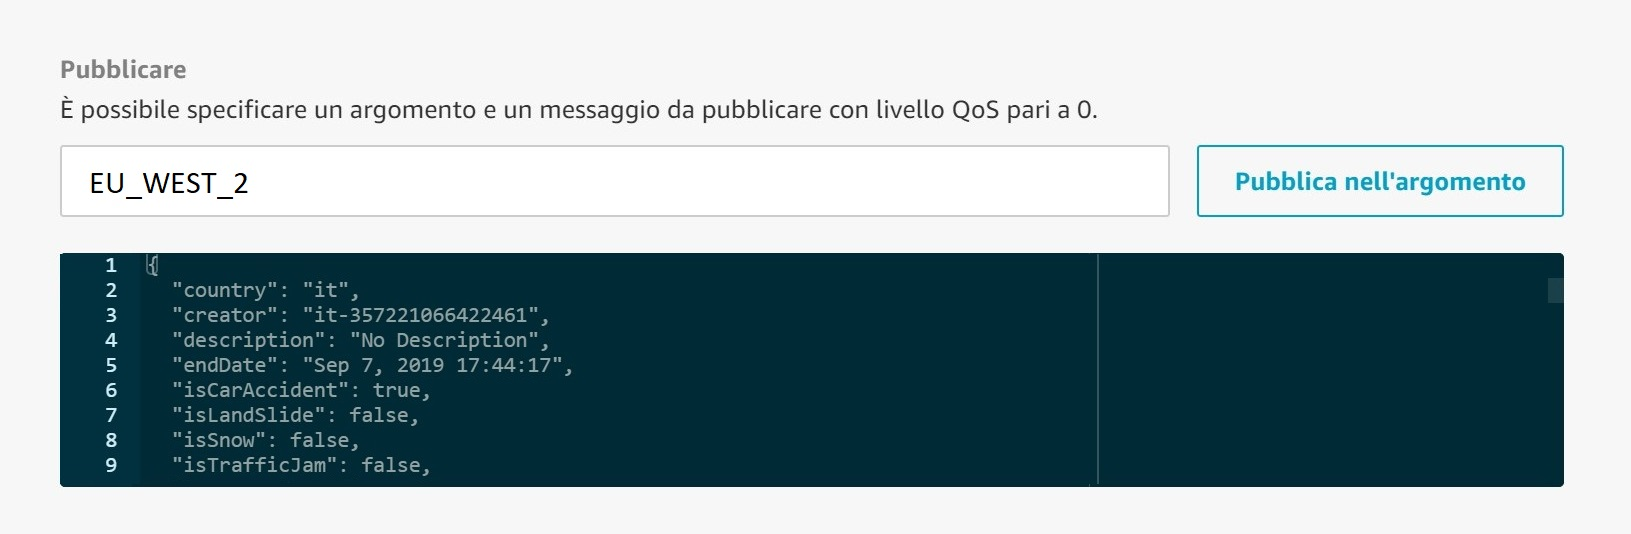
\includegraphics[width=1\columnwidth]{images/_5}
	\end{center}
	\caption{Pubblicazione nel Topic \textbf{EU\_WEST\_2}}
	\label{fig:_5}
\end{figure}
Dopo aver pubblicato il messaggio, nella sezione \textbf{Sottoscrivere} comparirà il messaggio appena ricevuto.
\begin{figure}
	\begin{center}
		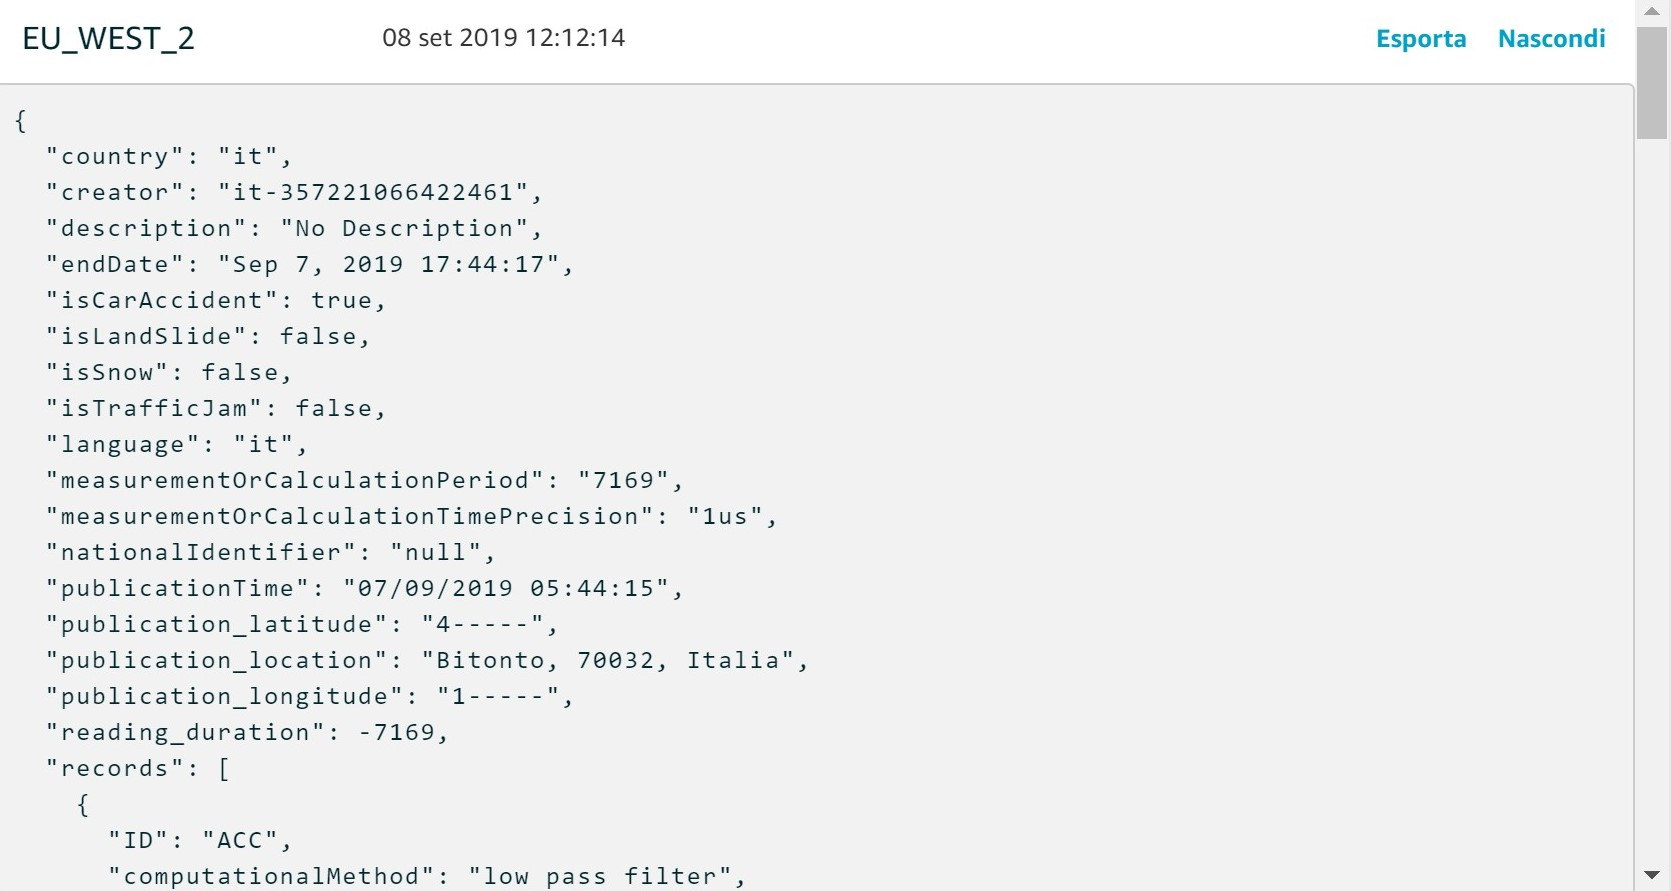
\includegraphics[width=1\columnwidth]{images/_6}
	\end{center}
	\caption{Ricezione del messaggio}
	\label{fig:_6}
\end{figure}
In maniera del tutto analoga, avverrà anche la comunicazione tra il Server IoT Core ed il Client Android. \\
Si noti come in \autoref{fig:_4}, \autoref{fig:_5} e \autoref{fig:_6} si è utilizzato come nome per il topic della pubblicazione \textbf{EU\_WEST\_2}. In realtà avremmo potuto ottenere lo stesso risultato e quindi stabilire la comunicazione tra client e server anche utilizzando un qualsiasi altro nome del topic, purchè il nome sul quale il Client pubblica i messaggi sia lo stesso sul quale il Server è in ascolto. Il motivo per cui sarà utilizzato il topic \textbf{EU\_WEST\_2} verrà spiegato nella \autoref{sec:aws_core}.

\subsubsection{Utilizzo della SDK}
Gli SDK (Software Development Kit) messi a disposizione dal team di sviluppo di AWS aiutano a connettere i dispositivi ad IoT Core in modo rapido e semplice.
Gli SDK di AWS IoT includono librerie open source, linee guida per gli
sviluppatori con esempi e guide alla portabilità, con cui è possibile creare soluzioni o prodotti IoT innovativi qualsiasi piattaforma hardware.\\
Gli SDK messi a disposizione dal team di AWS sono riferiti a specifiche architetture hardware e specifici linguaggi di programmazione e pertanto fuori dallo scope di questo capitolo che vuole invece fornire le linee guida generali di progettazione, indipendentemente dall'hardware e dal linguaggio utilizzato. Pertanto, nel \autoref{chap:quattro} saranno mostrati i dettagli implementativi dell' SDK per i dispositivi Android utilizzando il linguaggio di programmazione JAVA. \\
Qualora si vogliano ottenere i dettagli implementativi per altre piattaforme, si faccia riferimento alla documentazione ufficiale corredata anche da esempi applicativi (\url{https://docs.aws.amazon.com/it_it/iot/latest/developerguide/iot-dg.pdf}).
\begin{figure}
	\begin{center}
		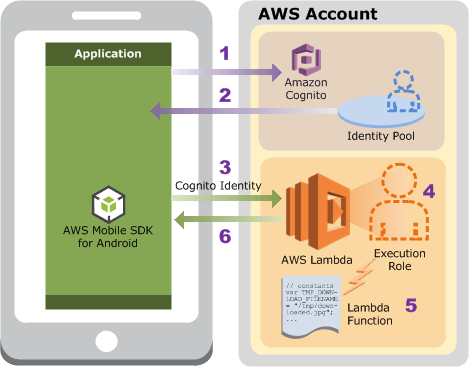
\includegraphics[width=0.5\columnwidth]{images/android_sdk}
	\end{center}
	\caption{Esempio dell'utilizzo dell'SDK messo a disposizione da AWS in Android per lo sviluppo di Lambda Application}
	\label{fig:android_sdk}
\end{figure}

\section{Database Architecture}
\label{sec:database}
In conclusione, l'utlima componente che è necessario progettare è il Database che si occuperà di raccogliere i dati provenienti da tutti i dispositivi IoT e transitanti attraverso la piattaforma cloud IoT Core. 
Il Database svolgerà un ruolo fodamentale in quanto non solo sarà il sistema di raccolta di tutti i dati provenienti da i dispositivi ma esso si occuperà anche di esporre questi stessi dati ad altre applicazioni che gli analizzeranno ed elaboreranno per trarne delle considerazioni e previsioni. Ulteriormente, i Database esporranno i dati in essi contenuti anche ad altri dispositivi IoT che dovessero interrogarli per ottenere informazioni sullo stato del traffico o in generale di eventi stradali.\\
Dal momento che la piattaforma Cloud che è stata scelta nella sezione precedente appartiene all'ecosistema AWS, è opportuno utilizzare un servizio di storage dei dati che appartenga allo stesso ecosistema in modo da sfruttare l'ampia documentazione e la facilità di interfacciamento dei due sistemi appartenenti allo stesso ecosistema. In tal caso, AWS mette a disposizione due servizi per lo storage dei dati:
\begin{itemize}
	\item \textbf{Amazon RDS: } Servizio per l'utilizzo di Database Relazionali (SQL)
	\item \textbf{Amazon DynamoDB: } Servizio per l'utilizzo di Database Non Relazionali (NoSQL)
\end{itemize}
La differenza sostanziale tra i due servizi consiste quindi nella architettura di Database nella quale si vogliono raccogliere i dati.\\
Si evidenzino quindi i requisiti che il Database deve soddisfare per il Software che si sta progettando in modo da vedere quali delle due servizi offerti da AWS sia più consono al progetto.\\
\begin{longtable}{|m{2cm}|m{12cm}|}
	\hline
	\textbf{Requisito} & \textbf{Descizione} \\
	\hline
	\textbf{D1} &   Il Database dovrà essere altamente scalabile per sopperire ad un numero di dispositivi e di entry nel database molto elevato \\
	\hline
	\textbf{D2} &   Il Database dovrà essere altamente performante per rispondere  in breve tempo alle query \\
	\hline
	\textbf{D3} &   Il Database dovrà supportare l'invio di query geo-referenziate \\
	\hline
	\textbf{D4} &   Il Database dovrà supportare e memorizzare diverse tipologie di dati provenienti da diversi dispositivi \\
	\hline
	\textbf{D5} &   Il Database dovrà essere progettato considerando il suo futuro utilizzo per la Big Data Analysis  \\
	\hline
	\caption{Analisi dei requisiti che la IoT Cloud Platform deve supportare}
	\label{tabel:requisiti_database}
\end{longtable}
Per capire quindi quale soluzione meglio si adatta ai requisiti del progetto in fase di sviluppo, è necessario effettuare una breve digressione sulle differenze tra le due architetture di un Database in modo da averne chiari i punti di forza ed i punti deboli di ciascuna architettura.\\

\subsection{Database Relazionali e Non Relazionali}
I Database Relazionali o \textbf{RDBMS} memorizzano i dati in tuple o record ovvero salvano i dati all'interno di tabelle. Ciascuna tabella ha un numero fisso di colonne e un numero variabile di righe (o record). Le colonne definiscono i dati degli attributi elle entità di una data tabella. Ad esempio, una tabella clienti avrà come colonne nome, cognome, indirizzo, telefono, e così via. Ogni riga nella tabella definisce un elemento effettivo costituito da valori per tutte le colonne.\\
Le tabelle hanno colonne speciali chiamate chiavi primarie (primary key), che contengono identificatori unici per ogni riga di una tabella. Le tabelle possono anche avere delle colonne chiamate chiavi esterne (foreign key), che contengono un riferimento chiave primaria di una riga su un’altra tabella (o anche sè stessa). Questi collegamenti tra righe sono chiamate associazioni (o relazioni, dall’inglese relationships) e sono la base del modello relazionale di un database.\\
\begin{figure}
	\begin{center}
		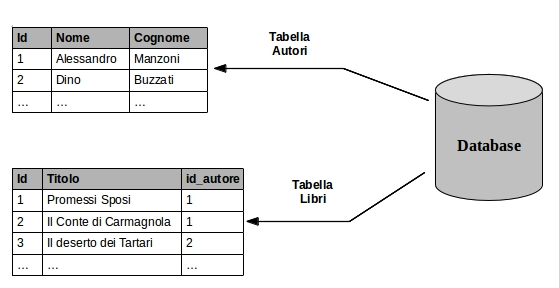
\includegraphics[width=0.5\columnwidth]{images/relational_db}
	\end{center}
	\caption{Esempio di un database relazionale}
	\label{fig:relational_db}
\end{figure}
I database relazionali trovano spazio d’applicazione quando si ha a che fare con dati strutturati, ovvero quando è facile creare una rappresentazione su tabella semplice e lineare, con un numero ridotto di relazioni. Inoltre, gli SQL sono praticamente obbligatori ogni volta che dobbiamo garantire integrità sui dati e le proprietà ACID in senso lato.\\
I Database Non Relazionali o \textbf{NRDBMS} utilizzano molteplici modelli di dati per accedere e gestire i dati, quali documento, grafo, chiave-valore, in memoria e ricerca. Questi tipi di database sono ottimizzati specificatamente per applicazioni che necessitano di grandi volumi di dati, latenza bassa e modelli di dati flessibili, ottenuti snellendo alcuni dei criteri di coerenza dei dati degli altri database. I database NoSQL sono una soluzione ideale per molte applicazioni moderne, quali dispositivi mobili, Web e videogiochi che richiedono database flessibili, scalabili, con prestazioni elevate ed altamente funzionali per offrire un'esperienza utente eccezionale.\\
I NoSQL sono estremamente versatili e quindi indicati in quelle situazioni in cui dobbiamo modellare il polimorfismo. Se si hanno entità tra loro tutte simili e che grossomodo portano la stessa informazione, ma con piccole differenze l’una dall’altra, con NoSQL il problema si risolve qualche manciata di minuti. In SQL, invece, è necessaria una soluzione decisamente più complessa. NoSQL è quindi ideale nel caso di dati abbastanza scorrelati e che tendono ad evolvere nel tempo; l’assenza di una struttura fissa permette di aggiungere nuovi tipi di dati (o modificare gli esistenti) senza dover mettere mano al database.
\begin{figure}
	\begin{center}
		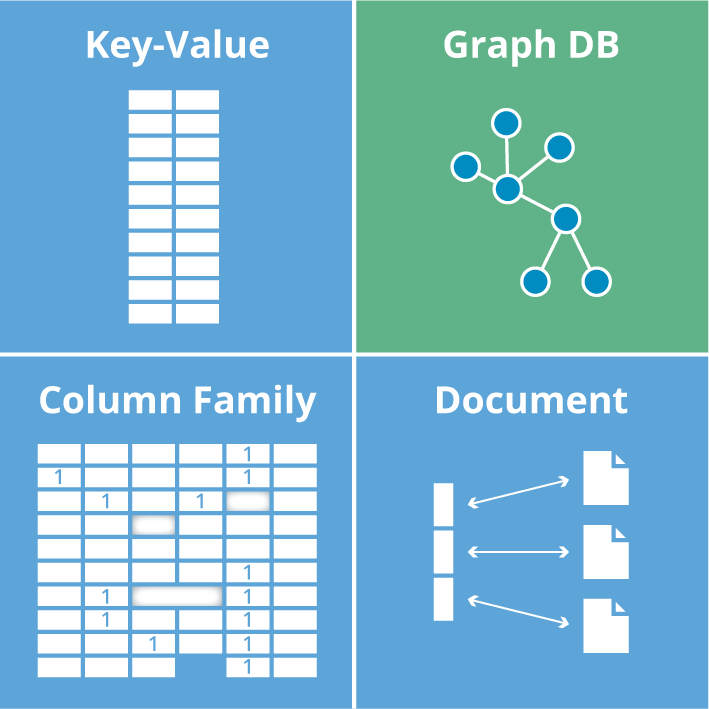
\includegraphics[width=0.45\columnwidth]{images/nonrelational_db}
	\end{center}
	\caption{Esempio di un database non relazionale}
	\label{fig:nonrelational_db}
\end{figure}

\subsection{Query Geo-Referenziate}
Una delle prerogative principali che il Database deve supportare sono la possibilità di rispondere a query geo-referenziate. Questo significa che un utente debba essere in grado di interrogare il Database per ricevere i soli eventi avvenuti in una certa area geografica. Allo stesso modo, anche la analisi dei dati può essere effettuata in forma locale in modo da poter eventualmente fornire diverse previsioni e considerazioni per diverse aree geografiche in funzione delle prerogative di quella particolare area. Questo implica delle scelte progettuali che tengano conto di questa prerogativa in modo da ottimizzare questo aspetto nella costruzione dell'architettura del Database.\\
Notevoli sono gli sforzi della ricerca per lo studio delle migliori architetture di Database che garantissero ottime performance quando sottoposti a query geo-referenziate. Nei lavori \cite{famous:paper_detti_1} e \cite{famous:paper_detti_2} viene progettato uno Spatial Database di tipo ICN (Information Centric Networking) denominato OpenGeoBase. Attraverso l'architettura implementata, il Database può facilmente lavorare in maniera distribuita, usando anche differenti Database Engines in parallelo. In questo modo, si realizza una architetture multi-tenant nella quale diversi utenti e diversi processi possono concorrere indipendentemente all'uso del Database. Ulteriormente, in \cite{famous:paper_detti_1} e \cite{famous:paper_detti_3} si dimostra come una implementazione di una simile architettura di Database sia particolarmente adatta ad applicazioni di ITS (Intelligent Transportation System) in quanto consenta l'esecuzione di query geo-referenziate. OpenGeoBase memorizza i dati geo-referenziati in formato GeoJSON supportando così query riferite ad una certa area geografica. Nella fattispecie, le funzionalità implementate da OpenGeoBase sono:
\begin{itemize}
	\item Routing-by-name per l'invio di query e l'inserimento di nuovi dati
	\item In-Networking caching per velocizzare le query e ridurre i tempi di calcolo del Database Engine
	\item Sicurezza di tipo Data-Centric per il supporto di applicazioni multi-tenant
\end{itemize}
Gli Spatial Database sono solitamente implementati come estensioni o plug-in di DBMS (Database Management System) generici. Tuttavia, in quanto Database Relazionali di tipo SQL, queste soluzioni sono affette da problemi di performamnces nel momento in cui le simensioni del Database aumentano. Pertanto, per grandi raccolte di dati (Big Data), i Database NoSQL stanno sempre più prendendo piede rimpiazzando i Database Relazionali in quanto i Non Relazionali risultano più semplici da distribuire in diversi Server. Sebbene un DBMS Relazionale possa offrire un numero maggiore di strumenti per la gestione e creazione di query, in applicazioni dove sono richieste soltanto delle semplici operazioni di read/write su grosse moli di dati, i Database NoSQL sono ritenuti più adatti in quanto possono essere più facilmente distribuiti.
\begin{figure}
	\begin{center}
		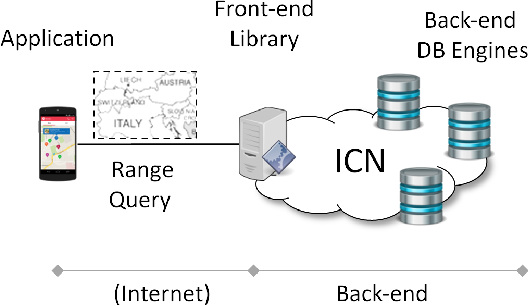
\includegraphics[width=0.6\columnwidth]{images/opengeobase_1}
	\end{center}
	\caption{Architettura di OpenGeoBase \cite{famous:paper_detti_1}}
	\label{fig:opengeobase_1}
\end{figure}
\begin{figure}
	\begin{center}
		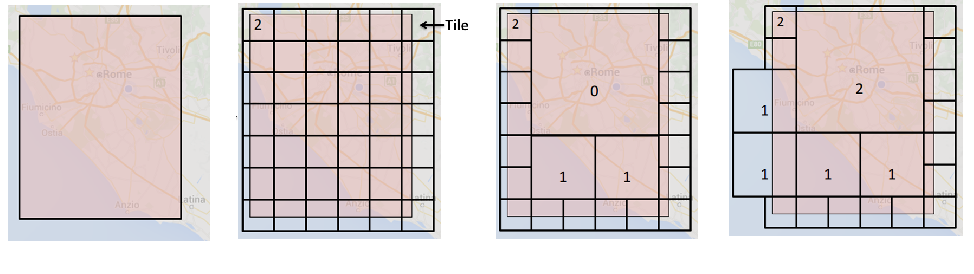
\includegraphics[width=0.8\columnwidth]{images/opengeobase_2}
	\end{center}
	\caption{Range-Query ed approcci di suddivisione della griglia basata su tre livelli 0,1,2 \cite{famous:paper_detti_1}}
	\label{fig:opengeobase_2}
\end{figure}


Alla luce di quanto detto, è subito evidente che una simile architettura di Database proposta in \cite
{famous:paper_detti_1} e \cite{famous:paper_detti_2} bene si adatti ai requisiti del sistema in fase di progettazione illustrati nella \autoref{tabel:requisiti_database}. Pertanto, alla luce del confronto tra Database Relazionali e Non, ed al fine di rendere il sistema in fase di sviluppo compatibile con l'implementazione di uno Spatial Database come OpenGeoBase, la scelta è ricaduta sull'utilizzo di un Database Non Relazionale e quindi NoSQL. Pertanto, dall'ecosistema AWS si è scelto di utilizzare Amazon DynamoDB.

\subsection{Amazon DynamoDB}
\label{subsec:dynamodb}
Amazon DynamoDB è il servizio di memorizzazione dei dati in Database Non Relazionali di tipo NoSQL. DynamoDB supporta i modelli di dati di tipo documento e di tipo chiave-valore ed è quindi adatto alla memorizzazione dei dati in formato JSON.\\
DynamoDB supporta due tipi di chiavi primarie:
\begin{itemize}
	\item \textbf{Partition key: } Una semplice chiave primaria, composta da un attributo chiamato \textit{partition key}. Gli attributi in DynamoDB sono simili in molti modi ai campi o alle colonne di altre arcitetture di Database
	\item \textbf{Partition key and Sort key: } Si riferiscono ad una chiave primaria composta da due attributi. Il primo attributo è la partition key ed il secondo attributo è chiamato \textit{sort key}
\end{itemize}
\begin{figure}
	\begin{center}
		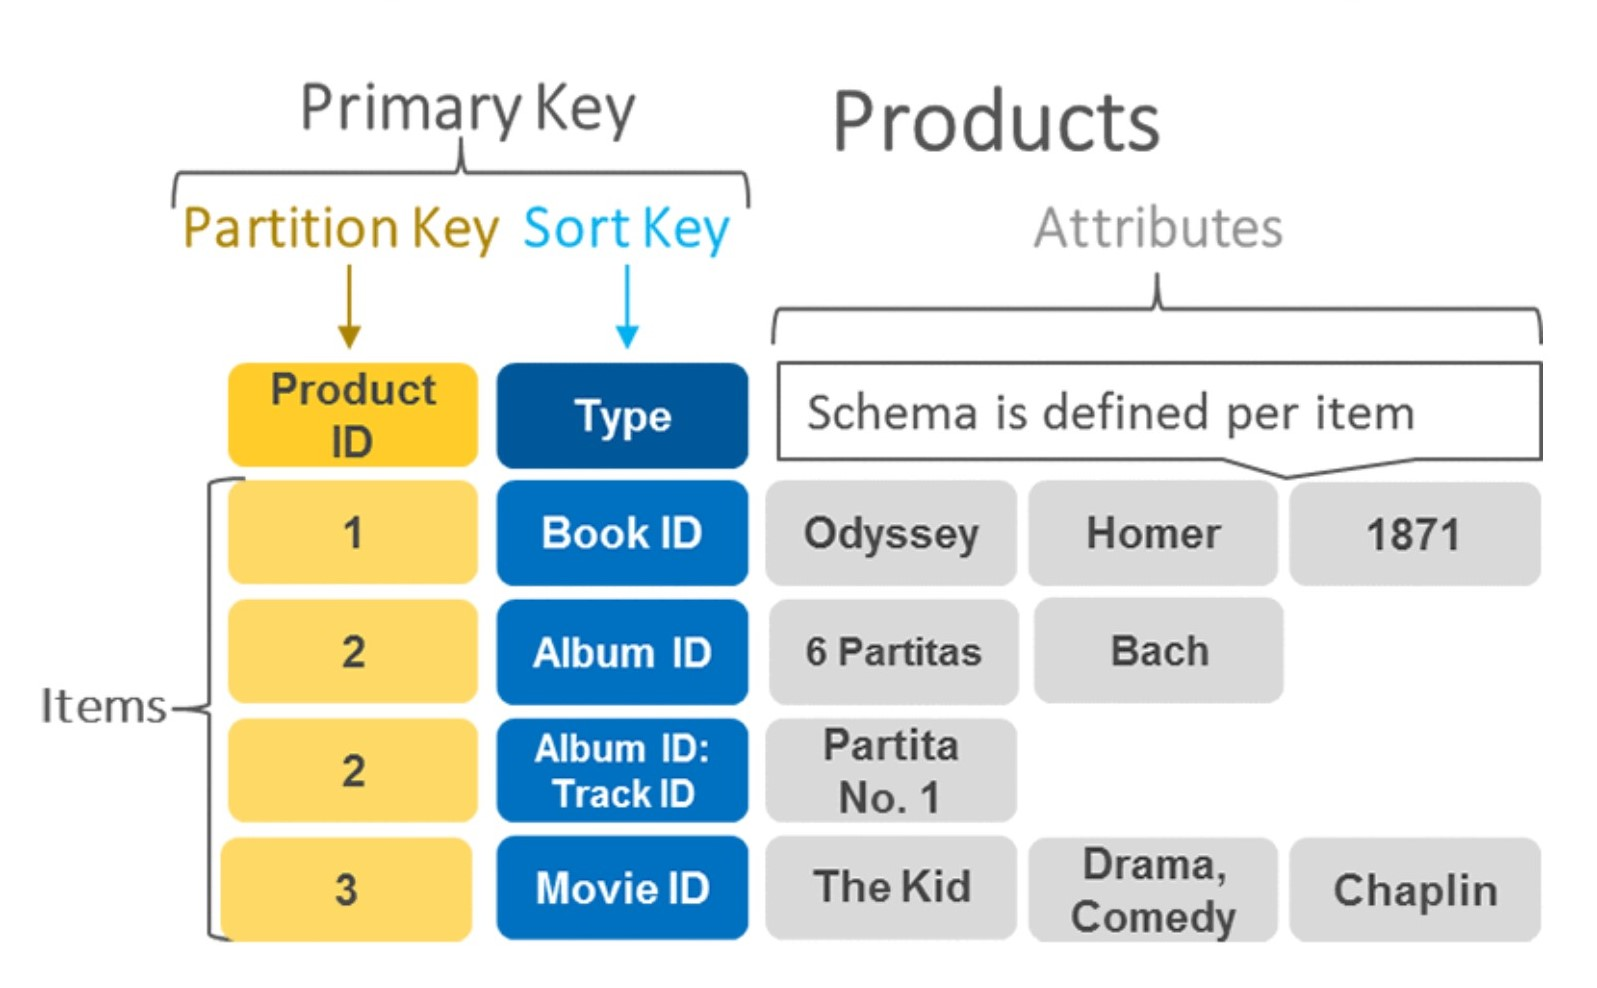
\includegraphics[width=0.7\columnwidth]{images/dynamodb_1}
	\end{center}
	\caption{Schema di una tabella in DynamoDB evidenziando i campi \textit{partition key} e \textit{sort key}}
	\label{fig:dynamodb_1}
\end{figure}
DynamoDB memorizza i dati come gruppi di attributi, chiamati \textit{items}. Gli \textit{items} sono simili alle righe o tuple o record in altri Database. Ciascun \textit{item} viene memorizzato e recuperato utilizzando la sua chiave primaria che deve quindi essere unica. Gli \textit{item} sono inoltre memorizzati in unità da 10GB chiamate partitions come mostrato in \autoref{fig:dynamodb_2}. Pertanto, tutti gli \textit{item} aventi lo stesso partition key sono memorizzati insieme, cioè nella stessa partition e sono ordinati in funzione del valore della loro sort key.
\begin{figure}
	\begin{center}
		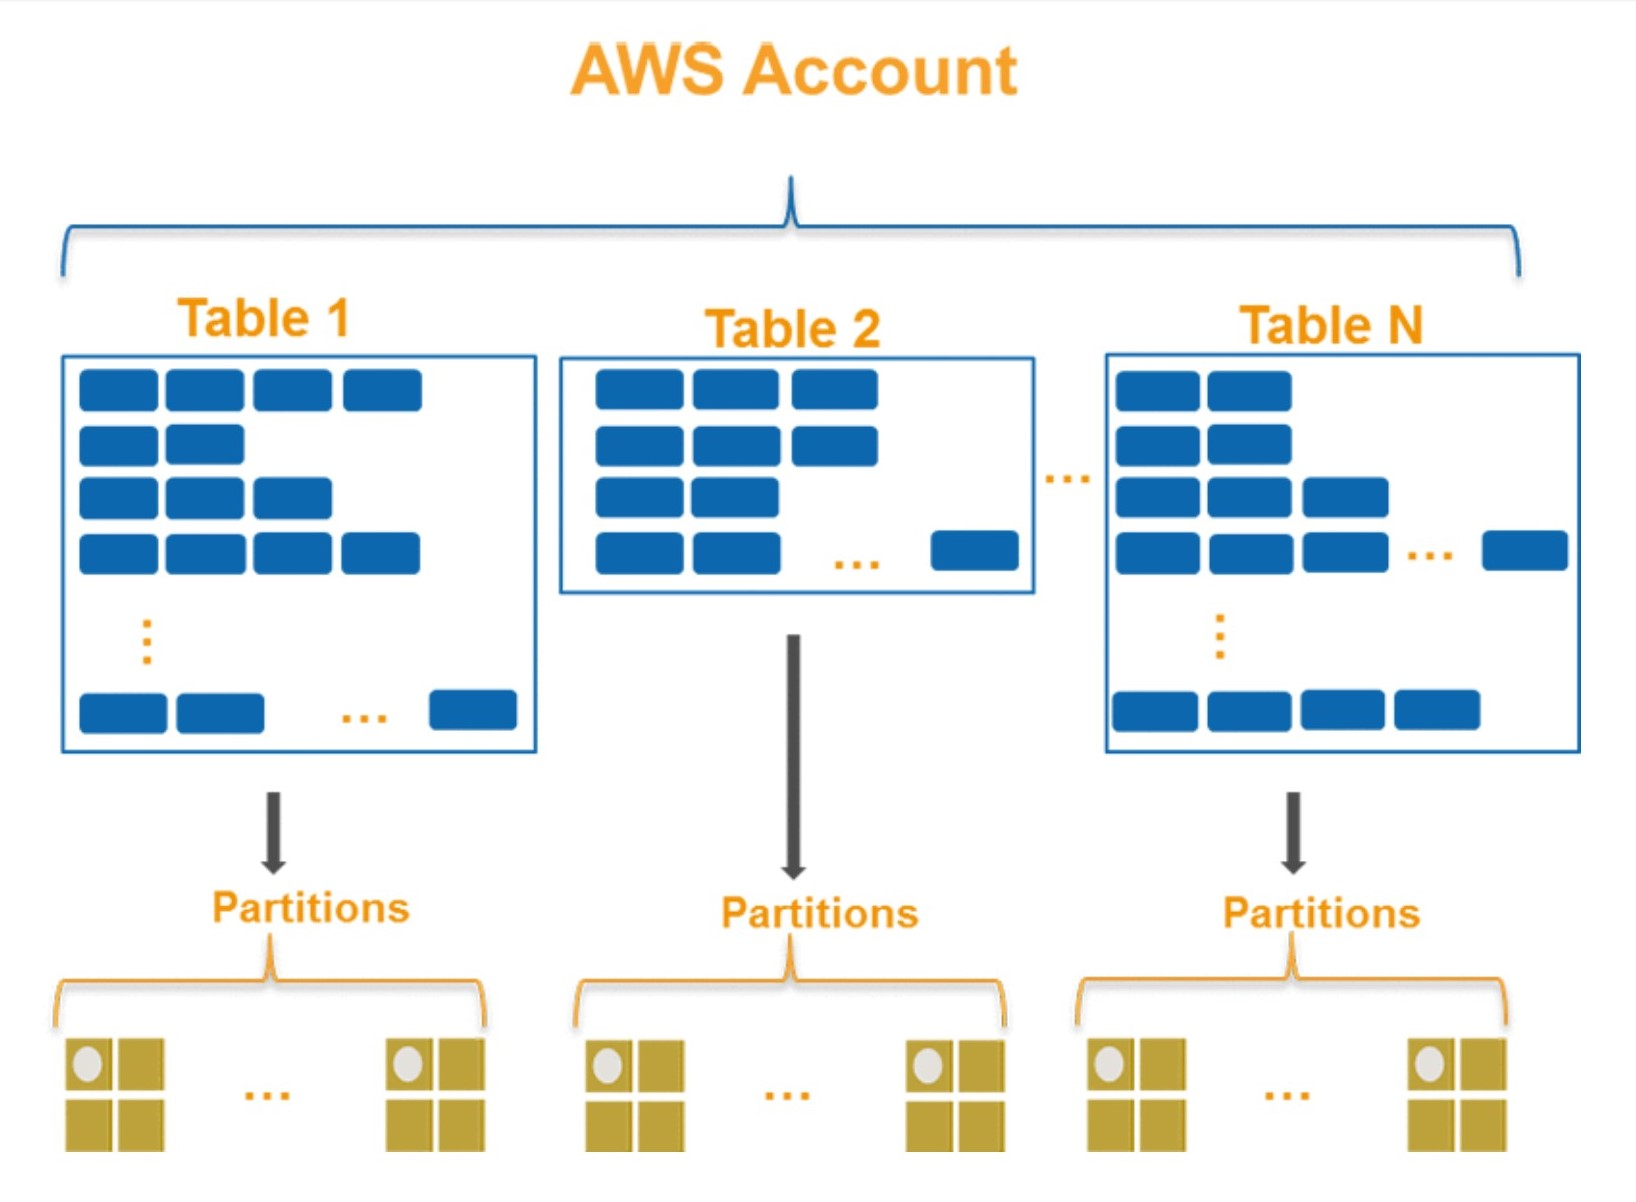
\includegraphics[width=0.6\columnwidth]{images/dynamodb_2}
	\end{center}
	\caption{Suddivisione di un Database in DynamoDB in tabelle e suddivisione delle tabelle in Partitions}
	\label{fig:dynamodb_2}
\end{figure}

A seguito della overview mostrata su DynamoDB, si ha ora a disposizione uno schema implementativo di un Database con DynamoDB. Pertanto, ora si può procedere al collegamento tra la Cloud Platform IoT Core progettata in precedenza ed il Database DynamoDB. Questa comunicazione sarà necessaria per fare in modo che i dati ricevuti dalla Cloud Platform IoT Core siano automaticamente memorizzati all'interno delle tabelle del Database che saranno poi utilizzate per le query degli uteni e per l'analisi dei dati. Una volta stabilita la comunicazione tra IoT Core e DynamoDB, nel \autoref{chap:quattro} sarà mostrata una implementazione di questa comunicazione e come sia possibile interrogare DynamoDB da uno smartphone android per visualizzarne i dati.\\
Per stabilire il collegamento tra IoT Core e DynamoDB è necessario creare una \textbf{regola} in DynamoDB che consenta di recuperare informazioni da un messaggio MQTT in ingresso e di scriverle in una tabella DynamoDB. I passi da seguire sono quindi:
\begin{itemize}
	\item Creazione di una nuova regola in AWS IoT Core
	\item Creazione di una nuova tabella in DynamoDB
	\item Creazione di un nuovo ruolo
	\item Test della comunicazione
\end{itemize}
Per avere un maggiore livello di dettaglio sull'implementazione di ciascuna fase, si faccia riferimento alla documentazione ufficiale \url{https://docs.aws.amazon.com/it_it/iot/latest/developerguide/iot-dg.pdf}.

\subsubsection{Creazione di una nuova Regola}
Con la creazione di una nuova Regola si vuole automatizzare il processo di comunicazione tra la piattaforma IoT Core ed il Database DynamoDB. In questo modo, ogni qual volta IoT Core riceve una nuova entry da dispositivi IoT, dopo aver eventualmente verificato e validato i dati, può memorizzarli in un Database per future elaborazioni ed analisi. \\
Per creare una nuova regola, si acceda alla piattaforma AWS IoT Core come spiegato nella \autoref{sec:iot_core} e nel riquadro di navigazione cliccare su \textit{Agisci} e quindi nella pagina \textit{Regole} cliccare su \textit{Crea una Regola}.A questo punto, nella pagina di creazione della nuova regola dovremmo inserire le caratteristiche della regola come Nome e Descrizione. Il campo \textit{Istruzione query della Regola} scegliere la versione più recente del campo Uso di SQL. Infine, nel campo \textit{Istruzioni query della Regola} va immessa la query in linguaggio SQL da eseguire quando viene attivata la regola.\\
\begin{figure}
	\begin{center}
		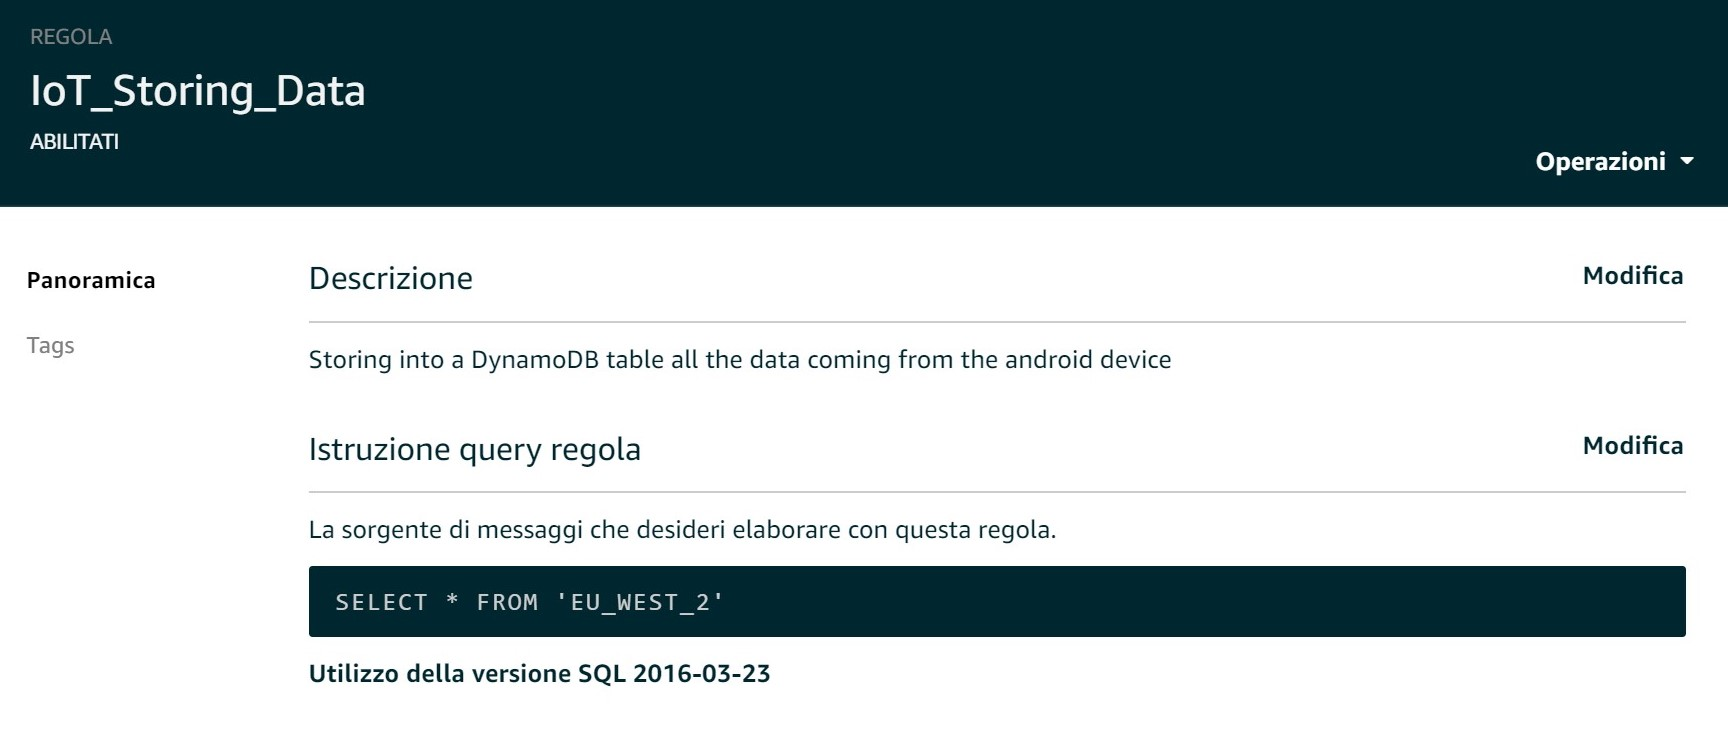
\includegraphics[width=0.7\columnwidth]{images/dynamodb_3}
	\end{center}
	\caption{Visualizzazione della Regola sul database DynamoDB}
	\label{fig:dynamodb_3}
\end{figure}
In questo caso, l'istruzione SQL che sarà eseguita consiste in una interrogazione di tutti i dati contenuti in una tabella di DynamoDB.

\subsubsection{Creazione di una nuova Tabella}
Una volta creata la regola in IoT Core, va ora creata e collegata ad una tabella di DynamoDB. Pertanto, nella pagina \textit{Seleziona un'operazione}, scegliere \textit{Inserisci un messaggio in una tabella DynamoDB} e quindi su \textit{Configura Operazione}.
\begin{figure}
	\begin{center}
		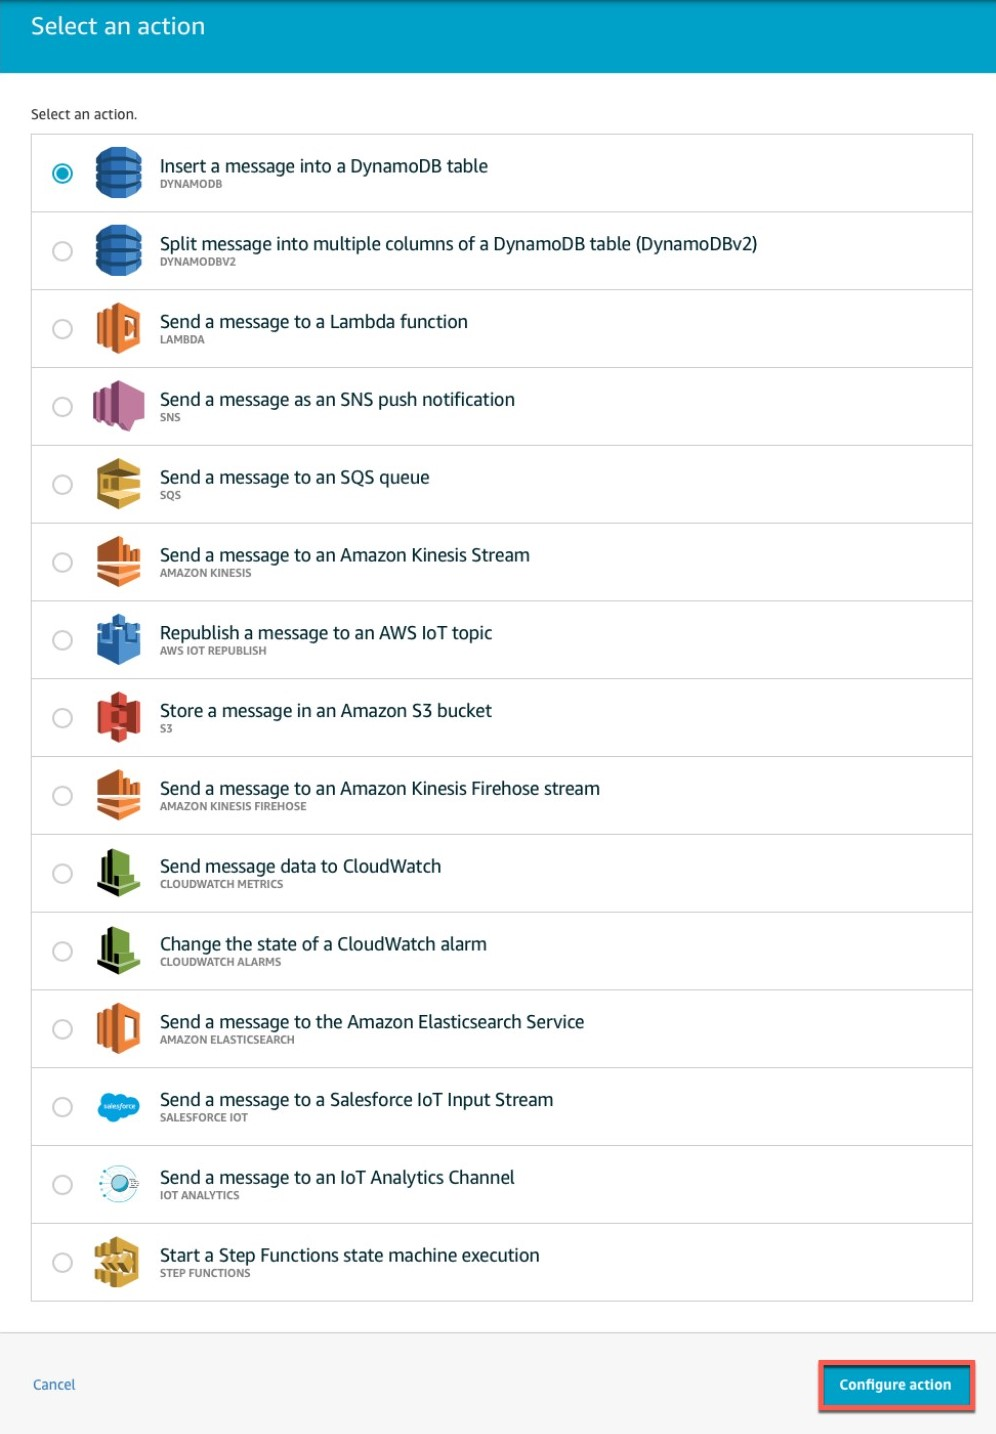
\includegraphics[width=0.58\columnwidth]{images/dynamodb_4}
	\end{center}
	\caption{Creazione di una nuova tabella}
	\label{fig:dynamodb_4}
\end{figure}
Nella pagina \textit{Configura Operazione} scegliere \textit{Crea una nuova Risorsa} e quindi nella pagina di DynamoDB scegliere \textit{Crea Tabella}.Nella pagina \textit{Crea tabella DynamoDB}, compilare i campi relativi alle informazioni della nuova tabella come Nome, Chiave di Partizione e Chiave di Ordinamento. Questi nomi, per testare un primo esempio di comunicazione, sono stati impostati a Row e PoistionInRow. Questi nomi assegnati alle colonne della tabella di DynamoDB dovranno rispettare quelli che saranno ricevuti all'interno del messaggio JSON ricevuto da DynamoDB.\\
Nel campo \textit{Partizione} e \textit{Chiave di ordinamento} scegliere String e quindi creare la nuova tabella con un click sul pulsante \textit{Crea}.\\
A questo punto, la tabella di DynamoDB è creata e si può chiudere la scheda del browser in cui è aperta la console Amazon DynamoDB.
A questo punto, nella console di AWS IoT Core precedentemente in fase di configurazione sarà visibile, nell'elenco delle tabelle, la tabella appena creata.


\subsubsection{Creazione di un nuovo Ruolo}
Una volta creata la nuova tabella in DynamoDB, è ora necessario fornire l'accesso alla lettura e scrittura di questa tabella ad IoT Core. Pertanto, nella console IoT Core, nella sezione \textit{Configura Operazione}, selezionare la tabella appena creata dall'elenco.\\
Quindi bisogna configurare i dettagli della comunicazione tra IoT Core e DynamoDB e, nel campo \textit{Partition Key} immettere \${row}. In questo modo, si indica alla regola di recuperare il valore dell'attributo row dal messaggio MQTT e di scriverlo nella colonna row della tabella DynamoDB. In \textit{Sort Key}, immettere \${pos}. In questo modo, il valore dell'attributo pos viene scritto nella colonna PositionInRow. Per impostazione predefinita, l'intero messaggio viene scritto in una
colonna della tabella denominata Payload. \\
Scegliere quindi \textit{Crea un nuovo ruolo} per procedere alla creazione di un nuovo ruolo da associare ad IoT Core per l'accesso alla tabella di DynamoDB. 
\begin{figure}
	\begin{center}
		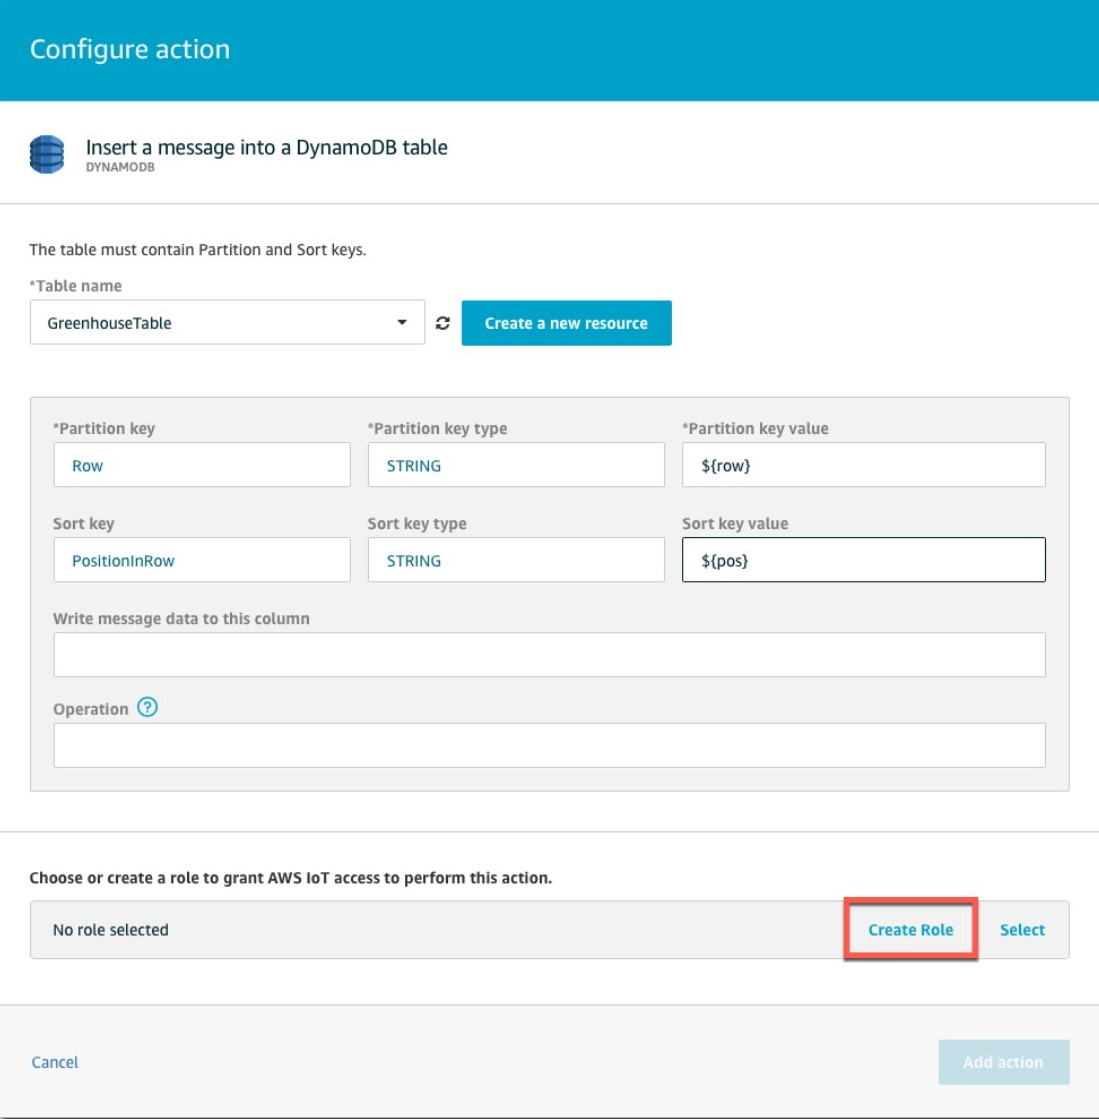
\includegraphics[width=0.41\columnwidth]{images/dynamodb_5}
	\end{center}
	\caption{Creazione di un nuovo ruolo}
	\label{fig:dynamodb_5}
\end{figure}

\subsubsection{Test della Comunicazione}
L'infrastuttura di DynamoDB è stata in questo modo creata e collegata ad IoT Core ed è quindi possibile testare la comunicazione tra AWS IoT Core e DynamoDB per verificare che nel momento in cui IoT Core riceva una nuova entry, questa venga automaticamente inviata alla tabella di DynamoDB che è stata in precedenza collegata. \\
Per fare questo bisogna recarsi nella sezione \textit{Test} e selezionare \textit{Pubblica in un Topic} e nella sezione topic immettere \textbf{EU\_WEST\_2} (lo stesso topic sul quale è in ascolto la regola precedentemente creata \autoref{fig:dynamodb_3}) e nell'area messaggio inserire un nuovo messaggio in formato JSON:
\begin{lstlisting}[language=Java, label= code:JSON_message, caption=Esempio di un possibile messaggio in formato JSON da salvare nel database]
	{
	  "row" : "0",
	  "pos" : "0",
	  "moisture" : "75"
	}
\end{lstlisting}
Quindi cliccare sul pulsante \textit{Pubblica nell'argomento} per inviare il messaggio a tutti i subscriber che sono in ascolto sul topic \textbf{EU\_WEST\_2}, tra i quali la regola di DynamoDB.\\
Infine, per verificare che la regola stia funzionando, accedere alla console di DynamoDB e nella sezione \textit{Tabelle}, cercare la tabella che è stata creata in precedenza e collegata alla regola. Si dovrà quindi vedere la nuova entry all'interno della tabella contenete proprio il messaggio appena pubblicato nel topic.\\
\begin{figure}
	\begin{center}
		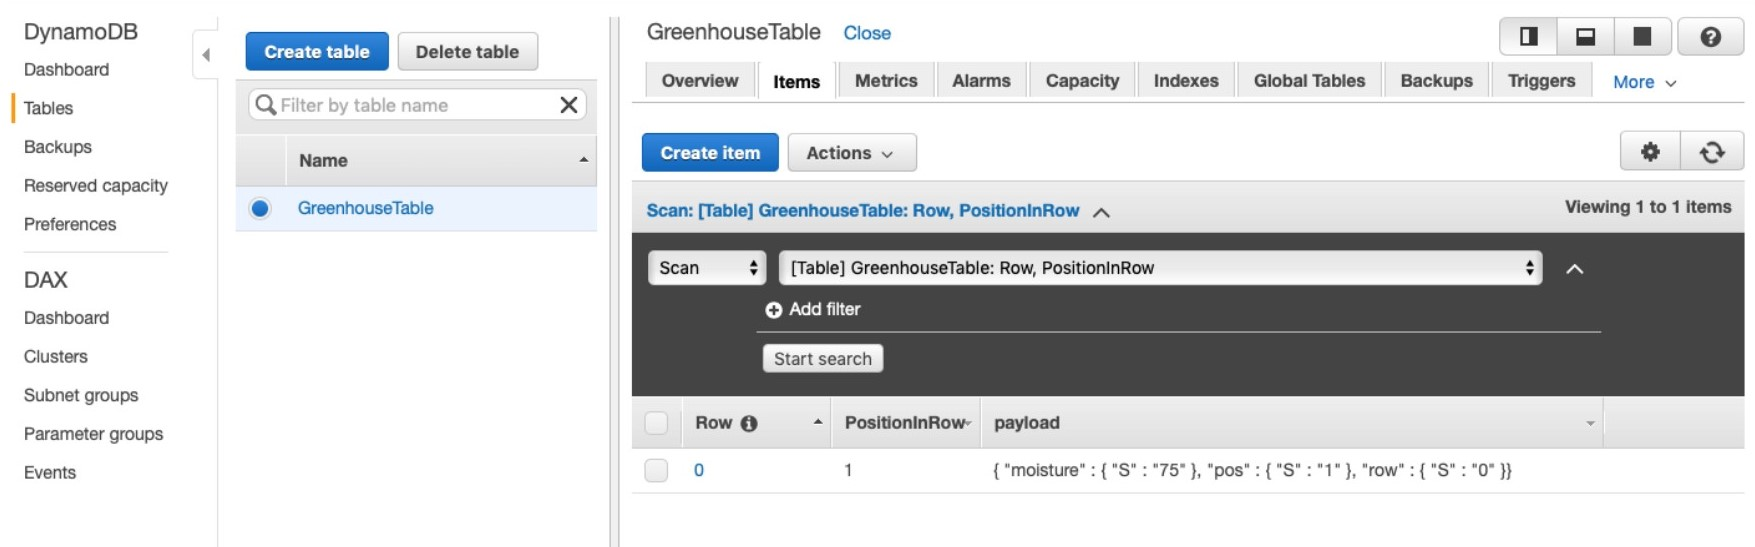
\includegraphics[width=1\columnwidth]{images/dynamodb_6}
	\end{center}
	\caption{Visualizzazione della nuova entry nella tabella}
	\label{fig:dynamodb_6}
\end{figure}
Si noti come, anche in questo caso \autoref{fig:dynamodb_6} si è utilizzato il topic \textbf{EU\_WEST\_2}, lo stesso utilizzato anche nella \autoref{subsubsec:com}. Sebbene il motivo per cui il nome del topic scelto è proprio \textbf{EU\_WEST\_2} sarà esplicitato in dettaglio nella \autoref{sec:aws_core}, per ora basti sapere che, questo stesso set-up della configurazione resta valido e funzionante con qualsiasi altro nome assegnato al topic, purchè i nomi lato Client, Server e lato Databse corrispondano.

